\documentclass[11pt]{article}		% Sets font size and document type
\usepackage{fontspec}				% Allows us to use custom fonts
\usepackage{graphicx}				% Does pictures
\usepackage{parskip}				% Removes paragraph indents
\usepackage{multicol}				% Allows for multiple columns
\usepackage{titlesec}				% Changes section title appearance
\usepackage{setspace}				% Allows you to set line spacing
\usepackage{amsmath}				% Maths typesetting
\usepackage[margin=20 mm]{geometry}	% Sets page margin
\usepackage[colorlinks=true,linkcolor=blue,citecolor=blue,urlcolor=blue]{hyperref}	
									% Allows for hypertext for references (links) - edited to hake links look like normal text rather than having a border
\doublespacing						% Double spaces - this annoys me but is unavoidable I think

%Add any more packages needed here:
\usepackage[justification=centering,font=small]{caption}	
									% Centres captions and makes them smaller
\usepackage[none]{hyphenat}			% Lines end cleanly - no hyphenation mid word
\usepackage{fancyhdr}				% Nicer headers/footers
\usepackage{amssymb}				% Allows for more maths symbols including not less than
\usepackage{wrapfig}				% Wrap figures

% Makes it so all equations have full sized numbers, independent of font size used		
\makeatletter
\def\tagform@#1{\maketag@@@{\normalsize(#1)\@@italiccorr}}
\makeatother

% There is some scope for changing the paragraph spacing and spacing around section headers if you are short of space

\graphicspath{{Images/}}	% Images are in a folder called 'Images'

% Set a variable for image height, so all images are the same size and easy to change
\newlength{\imageheight}	 % Creates the variable
\setlength{\imageheight}{0.3\textwidth}  % Sets the variable

\newcommand{\supercite}[1]{\textsuperscript{\cite{#1}}}		% New command to cite things in superscript without having to type it out every time

\newcommand{\figref}[1]{\hyperref[#1]{Figure \ref*{#1}}}    % New command to automatically fill out basic figures more easily

\newcommand{\equationref}[1]{\hyperref[#1]{Equation \ref*{#1}}}     % New command to automatically fill out equations more easily

% Use Arial
\setmainfont[
BoldFont=Arial Bold.ttf,
ItalicFont=Arial Italic.ttf,
BoldItalicFont=Arial Bold Italic.ttf
]{Arial.ttf}

% Have got this working with TexStudio now - need to change compiler from default to XeLaTeX (Options > Configure TexStudio > Build > Default Compiler > XeLaTeX)
% Will be slow at first, but once the fonts have installed should work more quickly

% Overleaf link - https://www.overleaf.com/project/5fce665153f1701e8414d47b
\begin{document}
	
	\flushleft
	\raggedright

	\begin{center}
		\vspace*{2cm}
		Michaelmas \& Hilary Term 2020 / 2021\\ % enter the date
		\vspace*{6cm}
		\huge{\textbf{3YP Project: Autonomous In-Pipe Inspection Robot}}\\ 
		\vspace*{6cm}
		\large{Monty Beresford, Louis Emanuel, Joshua Gei \& Jim Laney}
		\thispagestyle{empty} % Remove page number
	\end{center}

	\newpage
	
	\tableofcontents
	\thispagestyle{empty} % Remove page number
	\newpage

	\setcounter{page}{1}
	
	\section{Introduction - ENG + EEM}
Underground gas distribution pipelines span over 2 million km across global infrastructure\supercite{pct2020states}, comprising over 60\% of all underground pipelines\supercite{pct2020states}, and are essential in the transport of natural gas for domestic use or electricity generation. 

However, gas pipeline failures due to leaks as a result of wear-and-tear are commonplace. Unchecked leakages lead to transport delays, environmental damage, and potentially hazardous incidents\supercite{pct2020states} - in the US alone, there were a total of 1,051 serious incidents involving gas distribution and transmission from 1994-2013, \textbf{causing 319 fatalities and over US\$550 million in property damage}\supercite{pct2020states}!

Hence, adequate inspection and maintenance of gas pipelines are key priorities for gas distribution companies, which cumulatively spent \textbf{over US\$15.7 billion} on inspection, maintenance  and replacement of gas pipelines in 2019, and this amount is rising ~6\% year-on-year.\supercite{pct2020states}. 

Currently, the bulk of inspection and maintenance of buried gas pipelines is performed manually, with the aid of Pipeline Inspection Gauges (henceforth referred to as 'PIGs'), shown below in Figure 1. 

\begin{figure}[h]
			\centering
			\begin{multicols}{2}
				
\includegraphics[height=\imageheight]{placeholder}
				\caption{Excavation of entire pipeline required, and manual maintenance}
				\label{placeholder}
				\columnbreak
				
\includegraphics[height=\imageheight]{placeholder}
				\caption{Illustration of how PIGs are used}
				\label{placeholder}
			\end{multicols}
		\end{figure}
Nonetheless, the heavy amount of excavation required and the relatively slow and costly process of manual inspection poses pressing pain-points for gas distributors, as well as other stakeholders such as local councils and the general public. 

Hence, PipeDream will seek to address the target problems faced by our primary stakeholders with our product. 

	\subsection{Target Problems \textit{- Joshua Gei}}
We will first define the scope of our problem: PipeDream will target specifically \textbf{Tier 3 underground gas distribution pipelines in the UK}, using the pipeline assets category definition used by Ofgem, the Health and Safety Executive (HSE) and Gas Distribution Networks (GDNs)\supercite{pct2020states}. 

Table 1 shows the pipeline assets categories. 

    \begin{table}[h]
    \centering
  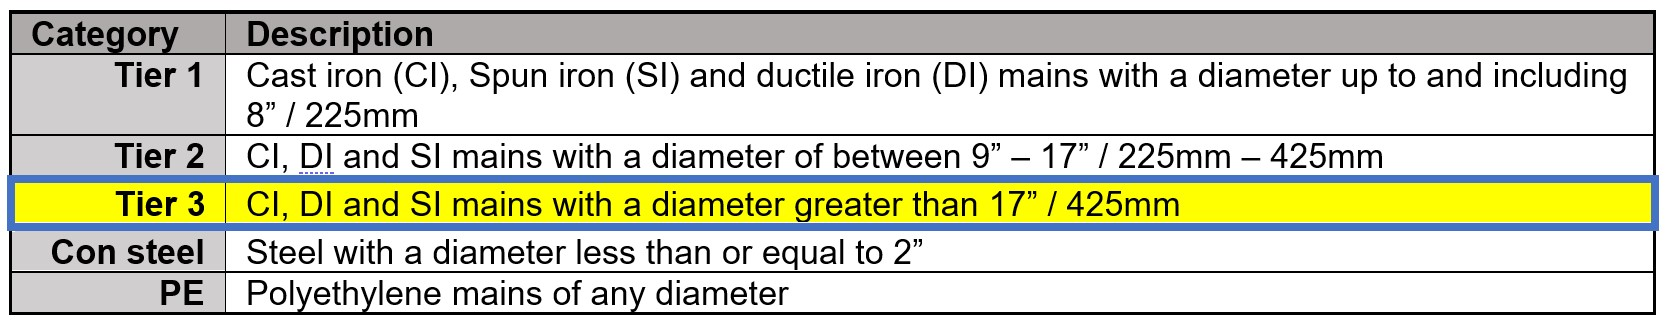
\includegraphics[width=\textwidth]{GasTiers}
  \caption{Pipeline Assets Category Definitions\supercite{pct2020states}.}
  \label{GasTiers}
    \end{table}
We reached out to a representative from Wales and West utilities (WWU), one of the 4 major GDNs in the UK, who pointed out that Tier 3 pipes in particular have pipe repairs increasing in volume and costs, have the largest proportion of buried mains reaching or beyond their expected asset life, and are the costliest to decommission and replace. Furthermore, Tier 3 mains are usually found in city locations, as opposed to other diameter types of pipelines, and cause considerable disruption to road users because multiple large excavations are required to complete the repairs.

Hence, a breakdown of the target problems faced by GDNs (our main customer), as well as other primary stakeholders, is as follows: 

\begin{enumerate}
   \item \textbf{Rising Costs}
   \begin{itemize}
     \item The individual entries are indicated with a black dot, a so-called bullet.
     \item The text in the entries may be of any length.
   \end{itemize}
   \item \textbf{Slow and Dangerous}
   \item \textbf{Obstructive}
   \item \textbf{Unable to inspect all types of pipes}
\end{enumerate}

	\subsection{Solution \textit{- Joshua Gei}}
	
	Robotic solutions are estimated to provide this amount of cost savings, but our own estimates are... 
	
	\section{Product Design - ENG}
	
	\subsection[Product Description]{Product Description - Jim Laney}
	
		The pipe inspection robot works in underground pipes in urban areas, with a pipe diameter from $457.2$ mm to $914.4$ mm and with pipes at any angle, providing a map of the pipe with the location of any failures to the operator. % 18 - 36 inches; Needs citation for pipe sizes?
		The robot reduces the disruption caused by having to dig up large areas of pipe for inspection, since the issue can be located and smaller, less disruptive work can be undertaken.
		It is intended to provide an inspection method for pipes which cannot be inspected by the current leading method, Pipe Inspection Gauges (PIGs), which only work in horizontal or near horizontal straight pipes\supercite{mills2017advances}.
		It enters a pipe using a launch tube, and travels autonomously along the inside of the pipe, checking for evidence of cracks and corrosion and logging their location for future maintenance.
		\\
		
		\begin{figure}[h] % Would like to do this as a text wrapped figure but that can be finnicky so would like to agree on this as a group before attempting it
			\centering
			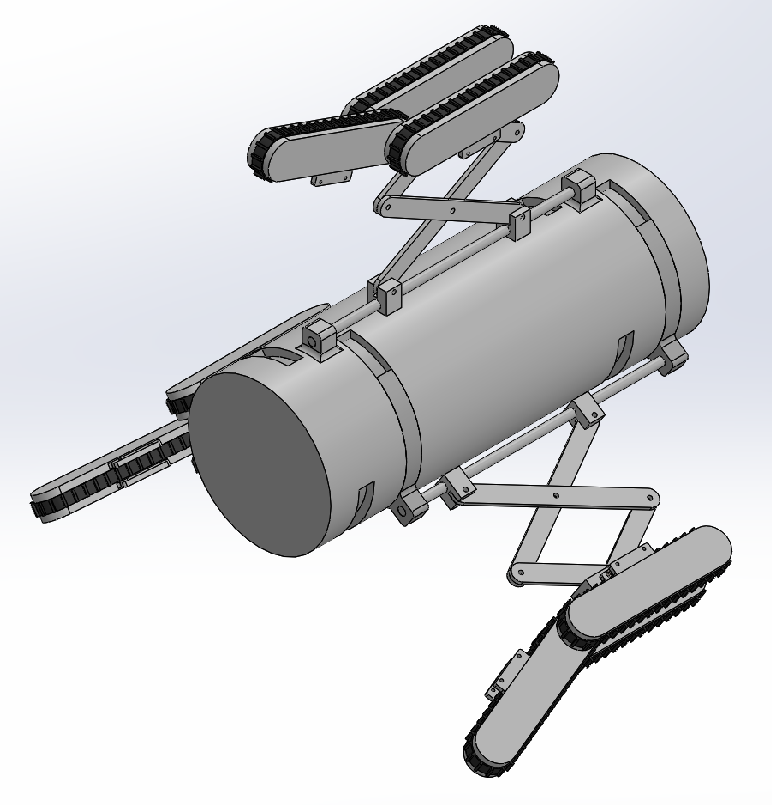
\includegraphics[trim={6cm 2cm 7cm 4cm},clip,height=\imageheight]{overviewCAD}
			\caption{3D CAD model of robot}
			\label{3DSketch}
		\end{figure}
		
		While inside the pipe, the robot uses three legs to maintain contact and provide the required normal force to move inside the pipe, as shown in \figref{3DSketch}.
		Two of these legs can """"""""be rotated to provide improved speeds over pipes at different angles, and all three legs can be extended and retracted to fit the pipe diameter the robot is currently in.
		It can navigate around bends and through pipes at different angles, without prior knowledge of the location or angle of these, and will automatically feedback to the control system in order to create an accurate map.
		\\
		The robot uses computer vision to identify cracks and corrosion, allowing it to mark where these occur for human maintenance, and then combines this with knowledge of its position to create a map of the pipe it has travelled and where issues have occurred.
		It can transmit its location using a small transmitter, which has a separate power supply so that if the robot breaks down it can be located with minimal excavation.
	
	\subsection[Patent Analysis]{Patent Analysis - Jim Laney}

		It was decided to look at patents classified as \verb|F16L55/26| - "Pigs or moles, i.e. devices movable in a pipe or conduit with or without self-contained propulsion means" or \verb|F16L2101/30| - "Inspecting, measuring or testing [as a use or application of pigs or moles]" as these are most similar to the purpose which the robot fulfils.
		In these patents the use of "pigs" refers to Pipeline Inspection Gauges (PIGs from here on), and moles are used as a synonymous term, and will thus also be referred to as PIGs from now on.
		While the robot is not a PIG as PIGs are typically unpowered and cannot deal with bends in the pipe, this is the closest patent classification to consider.
		\begin{figure}[h]
			\centering
			\begin{multicols}{2}
				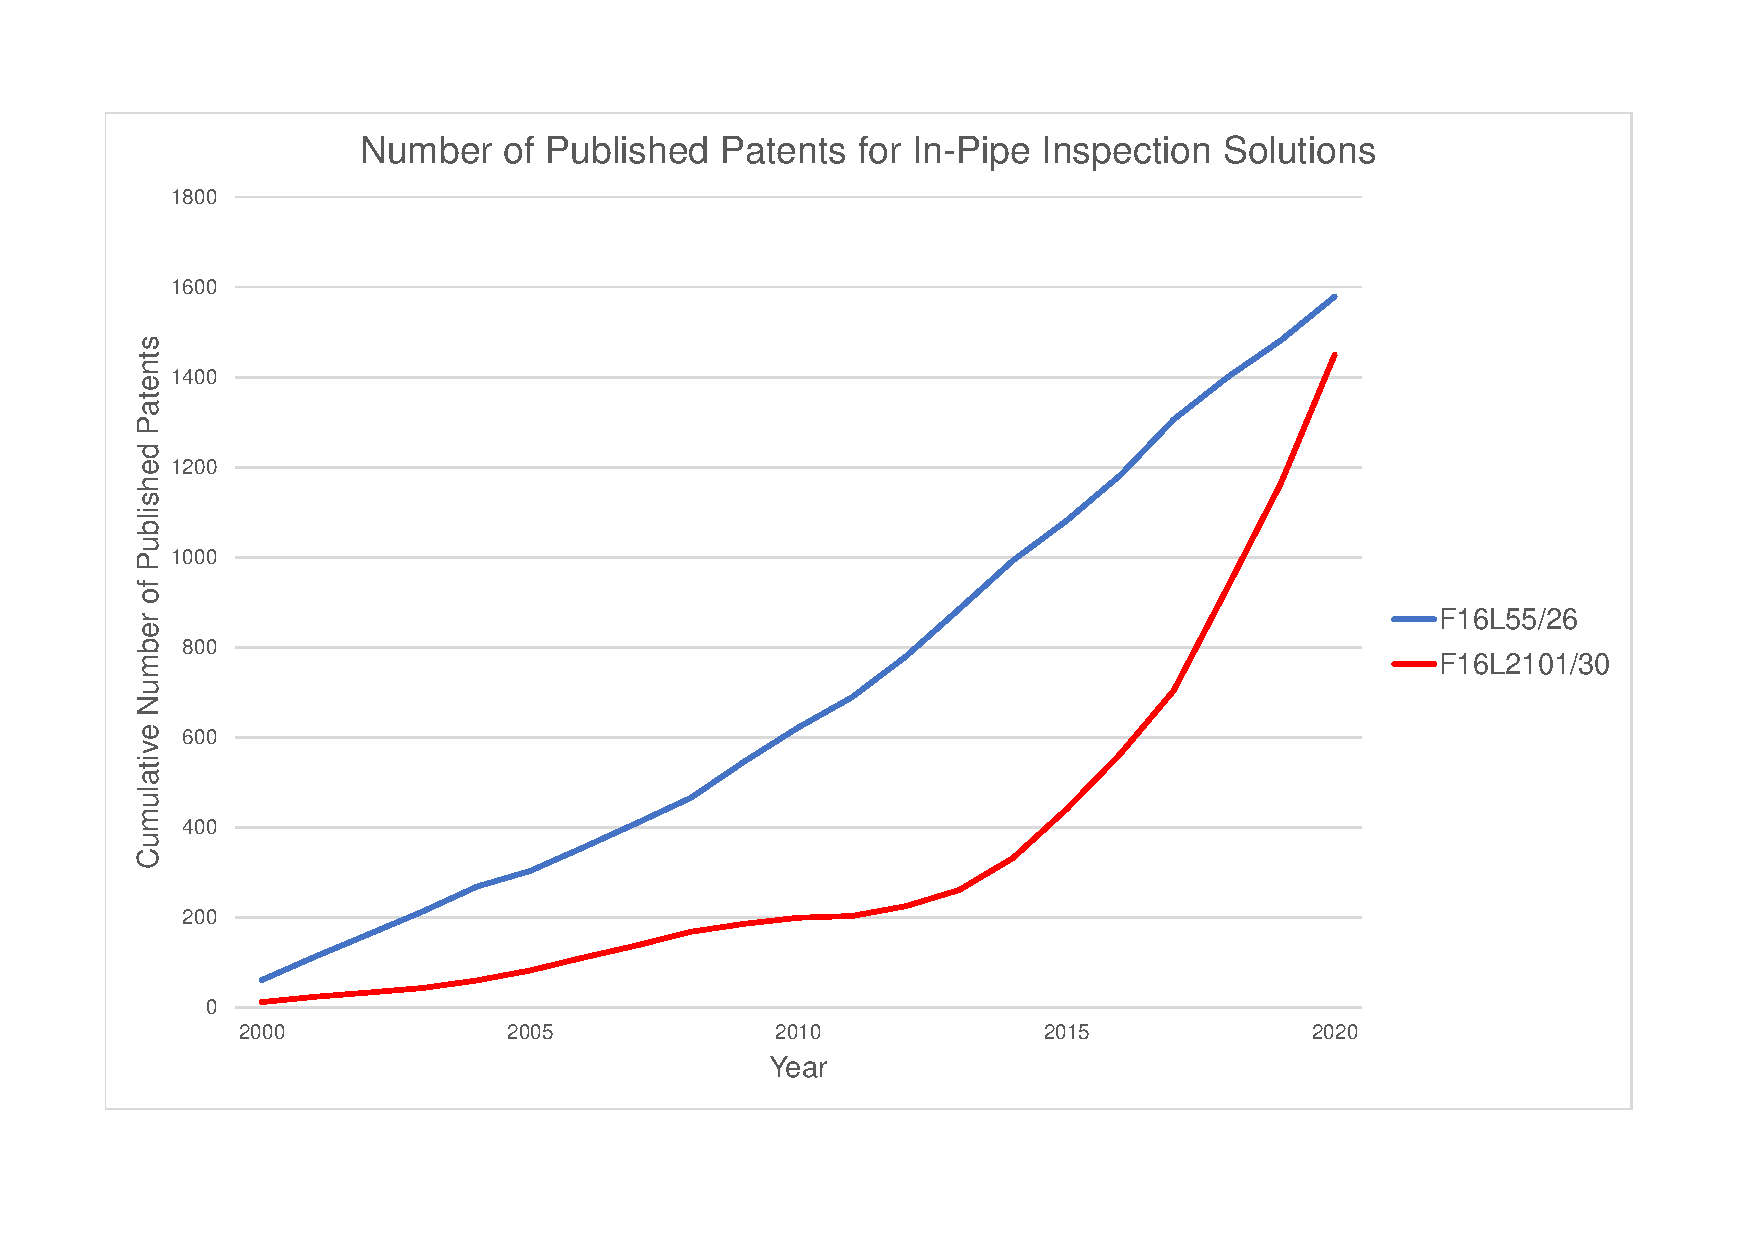
\includegraphics[height=\imageheight]{patentGraph}
				\caption{Cumulative number of published patents in the European Patent Office database classified as \texttt{F16L55/26}\supercite{patent26} or \texttt{F16L2101/30}\supercite{patent30} }
				\label{patentGraph}
				\columnbreak
				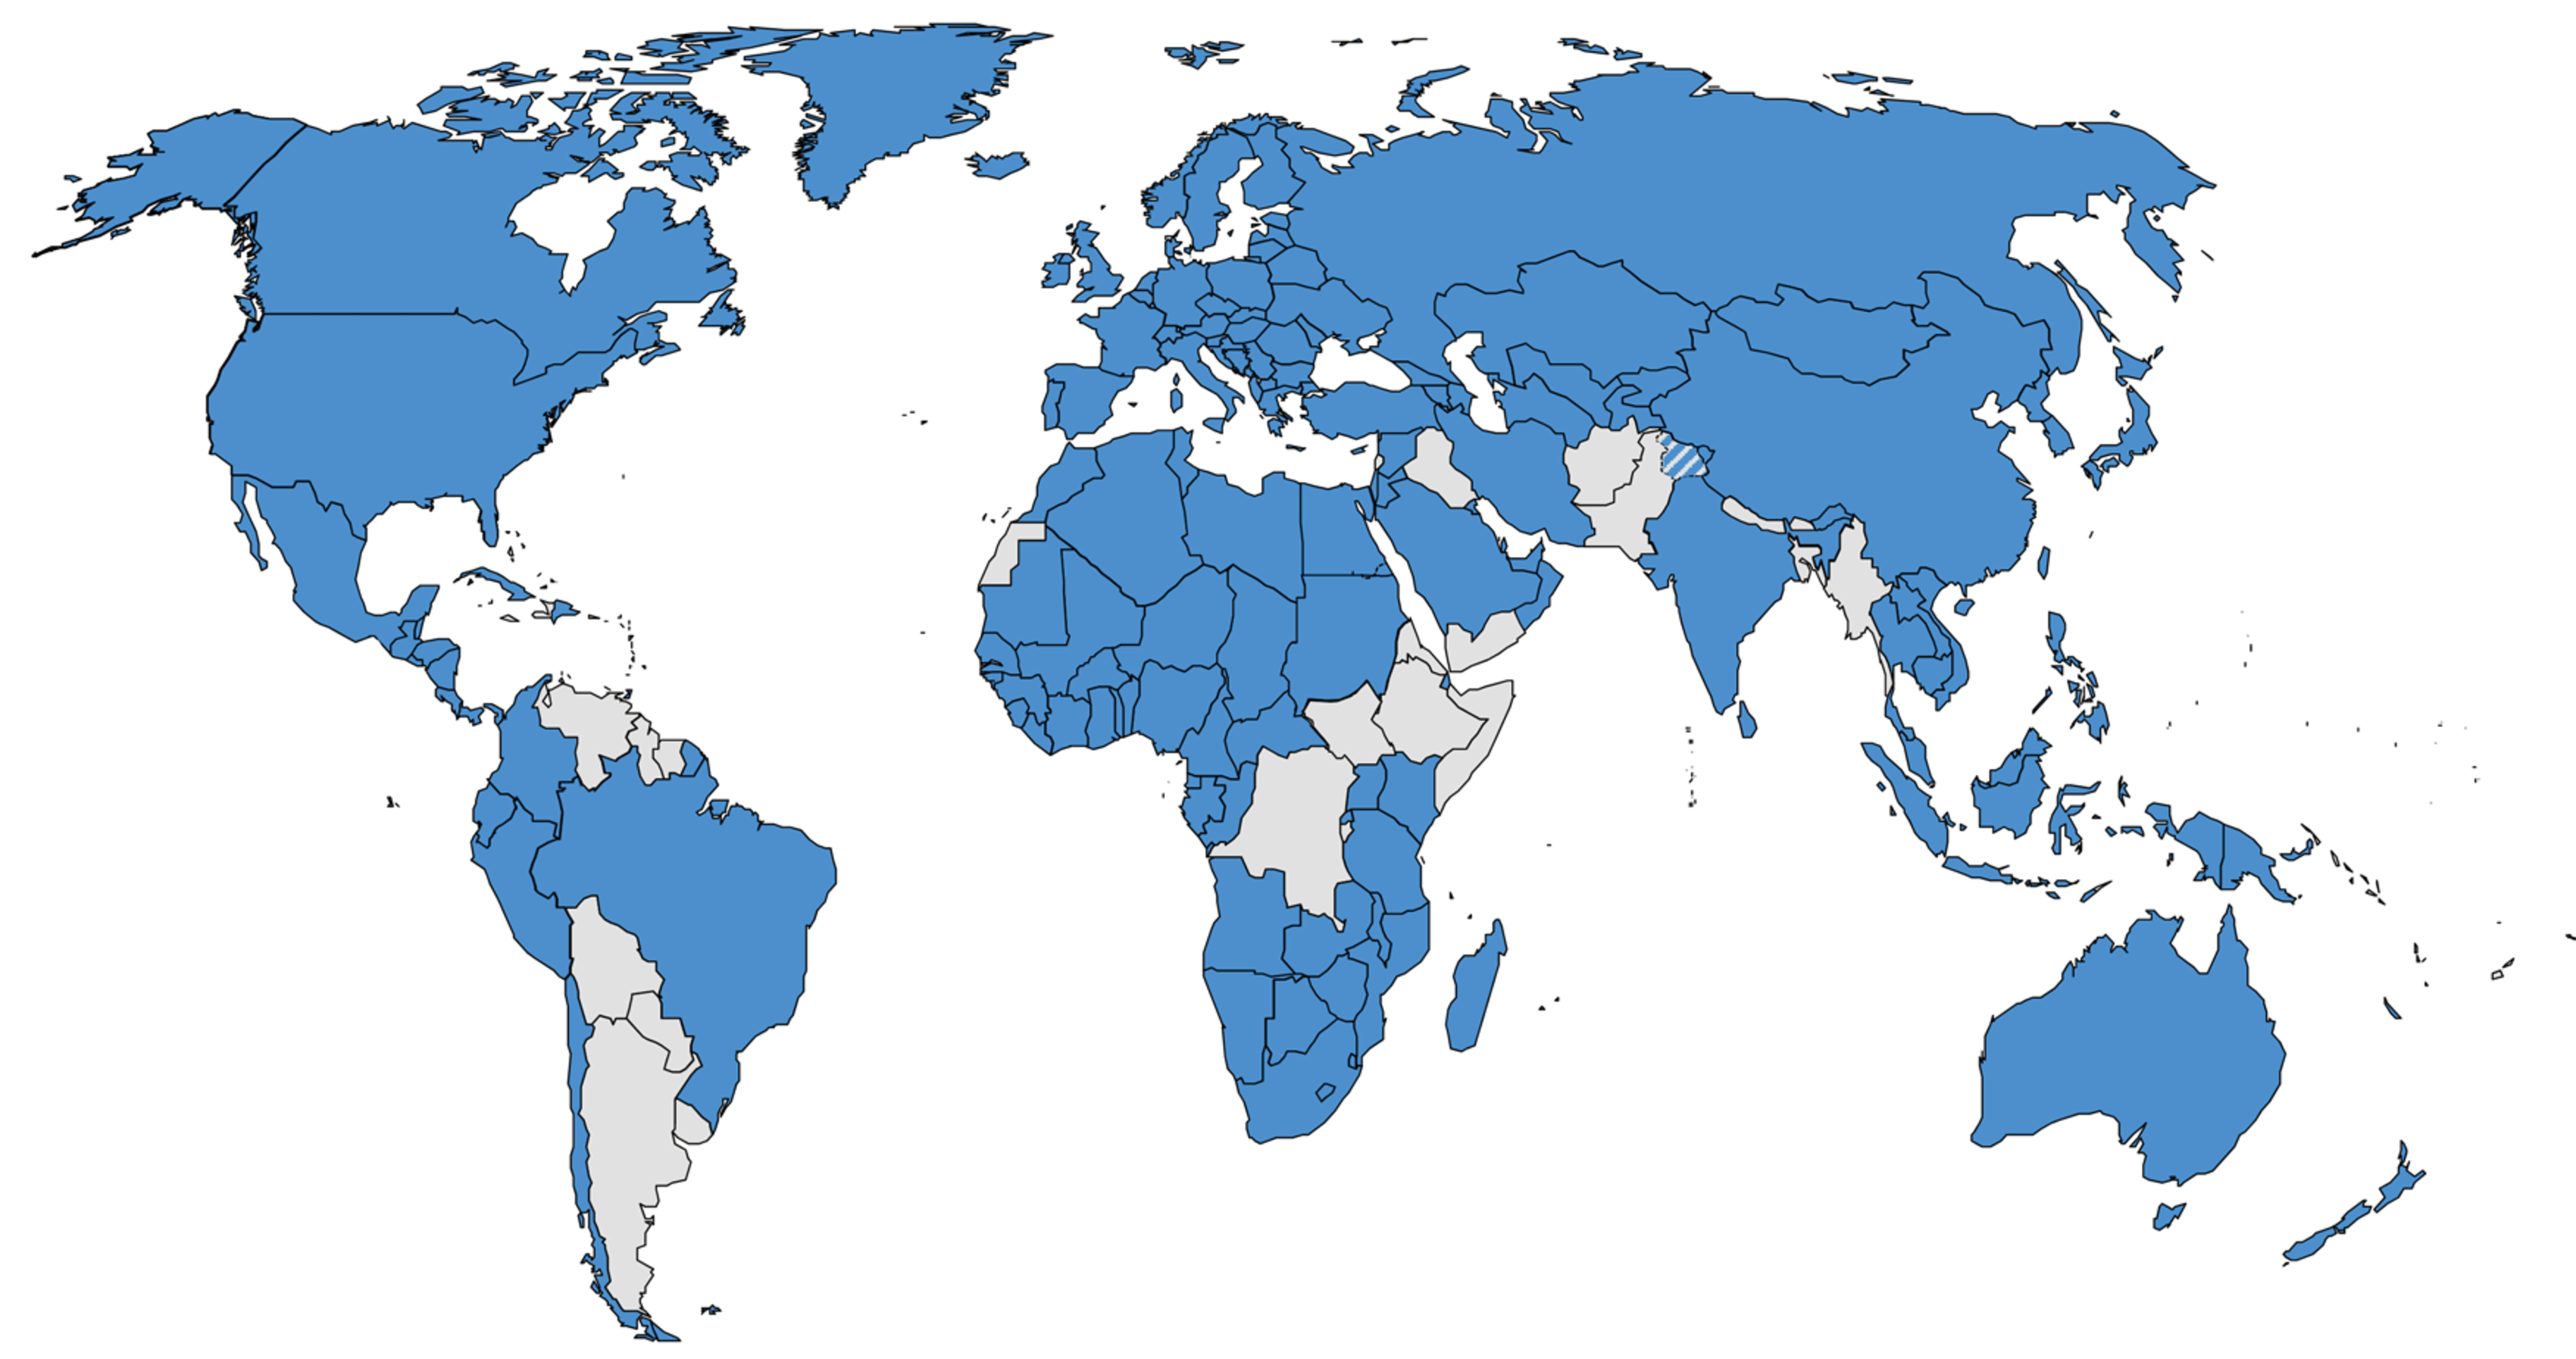
\includegraphics[height=\imageheight]{pctMap}
				\caption{Map of countries included in the Patent Cooperation Treaty (PCT)\supercite{pct2020states}}
				\label{pctMap}
			\end{multicols}
		\end{figure}
		\\
		As you can see from \figref{patentGraph}, the rate of patent publication in both classifications is still growing at a rapid rate, suggesting the technology is in a period of rapid innovation and development.
		This suggests that industry is still in the initial period of product design ferment, where no dominant design has occurred\supercite{christensen1998innovation}.
		Thus there is a much greater chance of survival, as this dominant design has not yet been established, and the space for new innovators is greater.
		While there is also a risk to entering the industry too early, the sustained period of development in the last 20 years suggests that period has passed.
		\\
		As well as this it is worth considering whether a patent should be filed in order to protect the robot design.
		The main barrier to this would be the cost of doing so, as the paperwork itself is not prohibitive, especially with the assistance of a patent law firm.
		However the cost to file a patent only in the United Kingdom is typically £4000 and usually takes 5 years to be filed\supercite{uk2020patenting}.
		As well as this it is a separate process to apply for a patent which will also apply overseas, such as applying through the Patent Cooperation Treaty (PCT).
		The PCT is treaty wich includes 153 states\supercite{pct2020states}, including the United Kingdom, United States and most of mainland Europe, as shown in \figref{pctMap}.
		However applying for a PCT patent can take even longer, and is even more expensive, up to £8000\supercite{mewburn2020international}, so it is important to ensure that the robot design is protected while applying for these patents.
		Thus it would be a good idea to apply for some less strict protection, such as a trademark, and ensure that all discussions of sensitive information occur under the binding of a Non-Disclosure Agreement.
		
	\subsection[Constraint Justification]{Constraint Justification}
		
		% Section about how we decided pipe diameters and other important things - gas pressure, etc?
	
	\section{Product Hardware - ENG}
	
		\subsection[Locomotion]{Locomotion - Jim Laney}
			
			%By Jim
			The main locomotion of the robot is a set of 3 legs with a pantograph mechanism  to allow for the adaptation to different diameters, with tracks at the end to drive the motion, as shown in \figref{legDesign}.
			There is one leg which remains stationary at the top of the robot, and two legs which are able to rotate about the body of the robot between $20^\circ$ and $90^\circ$ to the vertical.
			At the end of each leg there is a passive joint between the leg and the track to allow for the robot to travel along surfaces which are not perpendicular to the legs, such as around bends or over uneven surfaces.
			\\
			The length of the pantograph is controlled by the force from two opposing linear actuators, which extend to a given length to set the distance of the pantograph.
			The track at the end of the pantograph is connected to a freely turning joint, which can be measured using two angular encoders to give the angle $\phi$, shown in \figref{legDiagram}, with the springs acting to restore $\phi$ to $0^\circ$ when under no external effects.
			In addition to this, the tracks use an active compliance joint, as shown in \hyperref[activeCompliance]{Figures \ref*{activeCompliance} \& \ref*{unevenBehaviour}}, which allows for the robot to maintain maximum surface contact at all times.
			\\
			The active compliance joint consists of a torsional spring and radio-controlled servo motor, which are both attached around the same axis.
			However, the servo motor is attached to the rear tracks, whereas the spring is attached between the front track and the servo motor itself.
			When the robot passes over an uneven surface, the servo motor forces the front track down, maintaining contact with the pipe wall, as shown in \hyperref[unevenBehaviour]{Figure \ref*{unevenBehaviour}(a)}
			If instead the robot is in a section where the pipe wall is concave, the torsional spring will allow it to fold, shown in \hyperref[unevenBehaviour]{Figure \ref*{unevenBehaviour}(b)}, and maintaining contact with as much of the wall as possible.
			The active compliance joint also includes an angular encoder to tell how much the front track has been bent, allowing for the active compliance joint to be better controlled.
			\begin{figure}[h]
				\centering
				\begin{multicols}{2}
					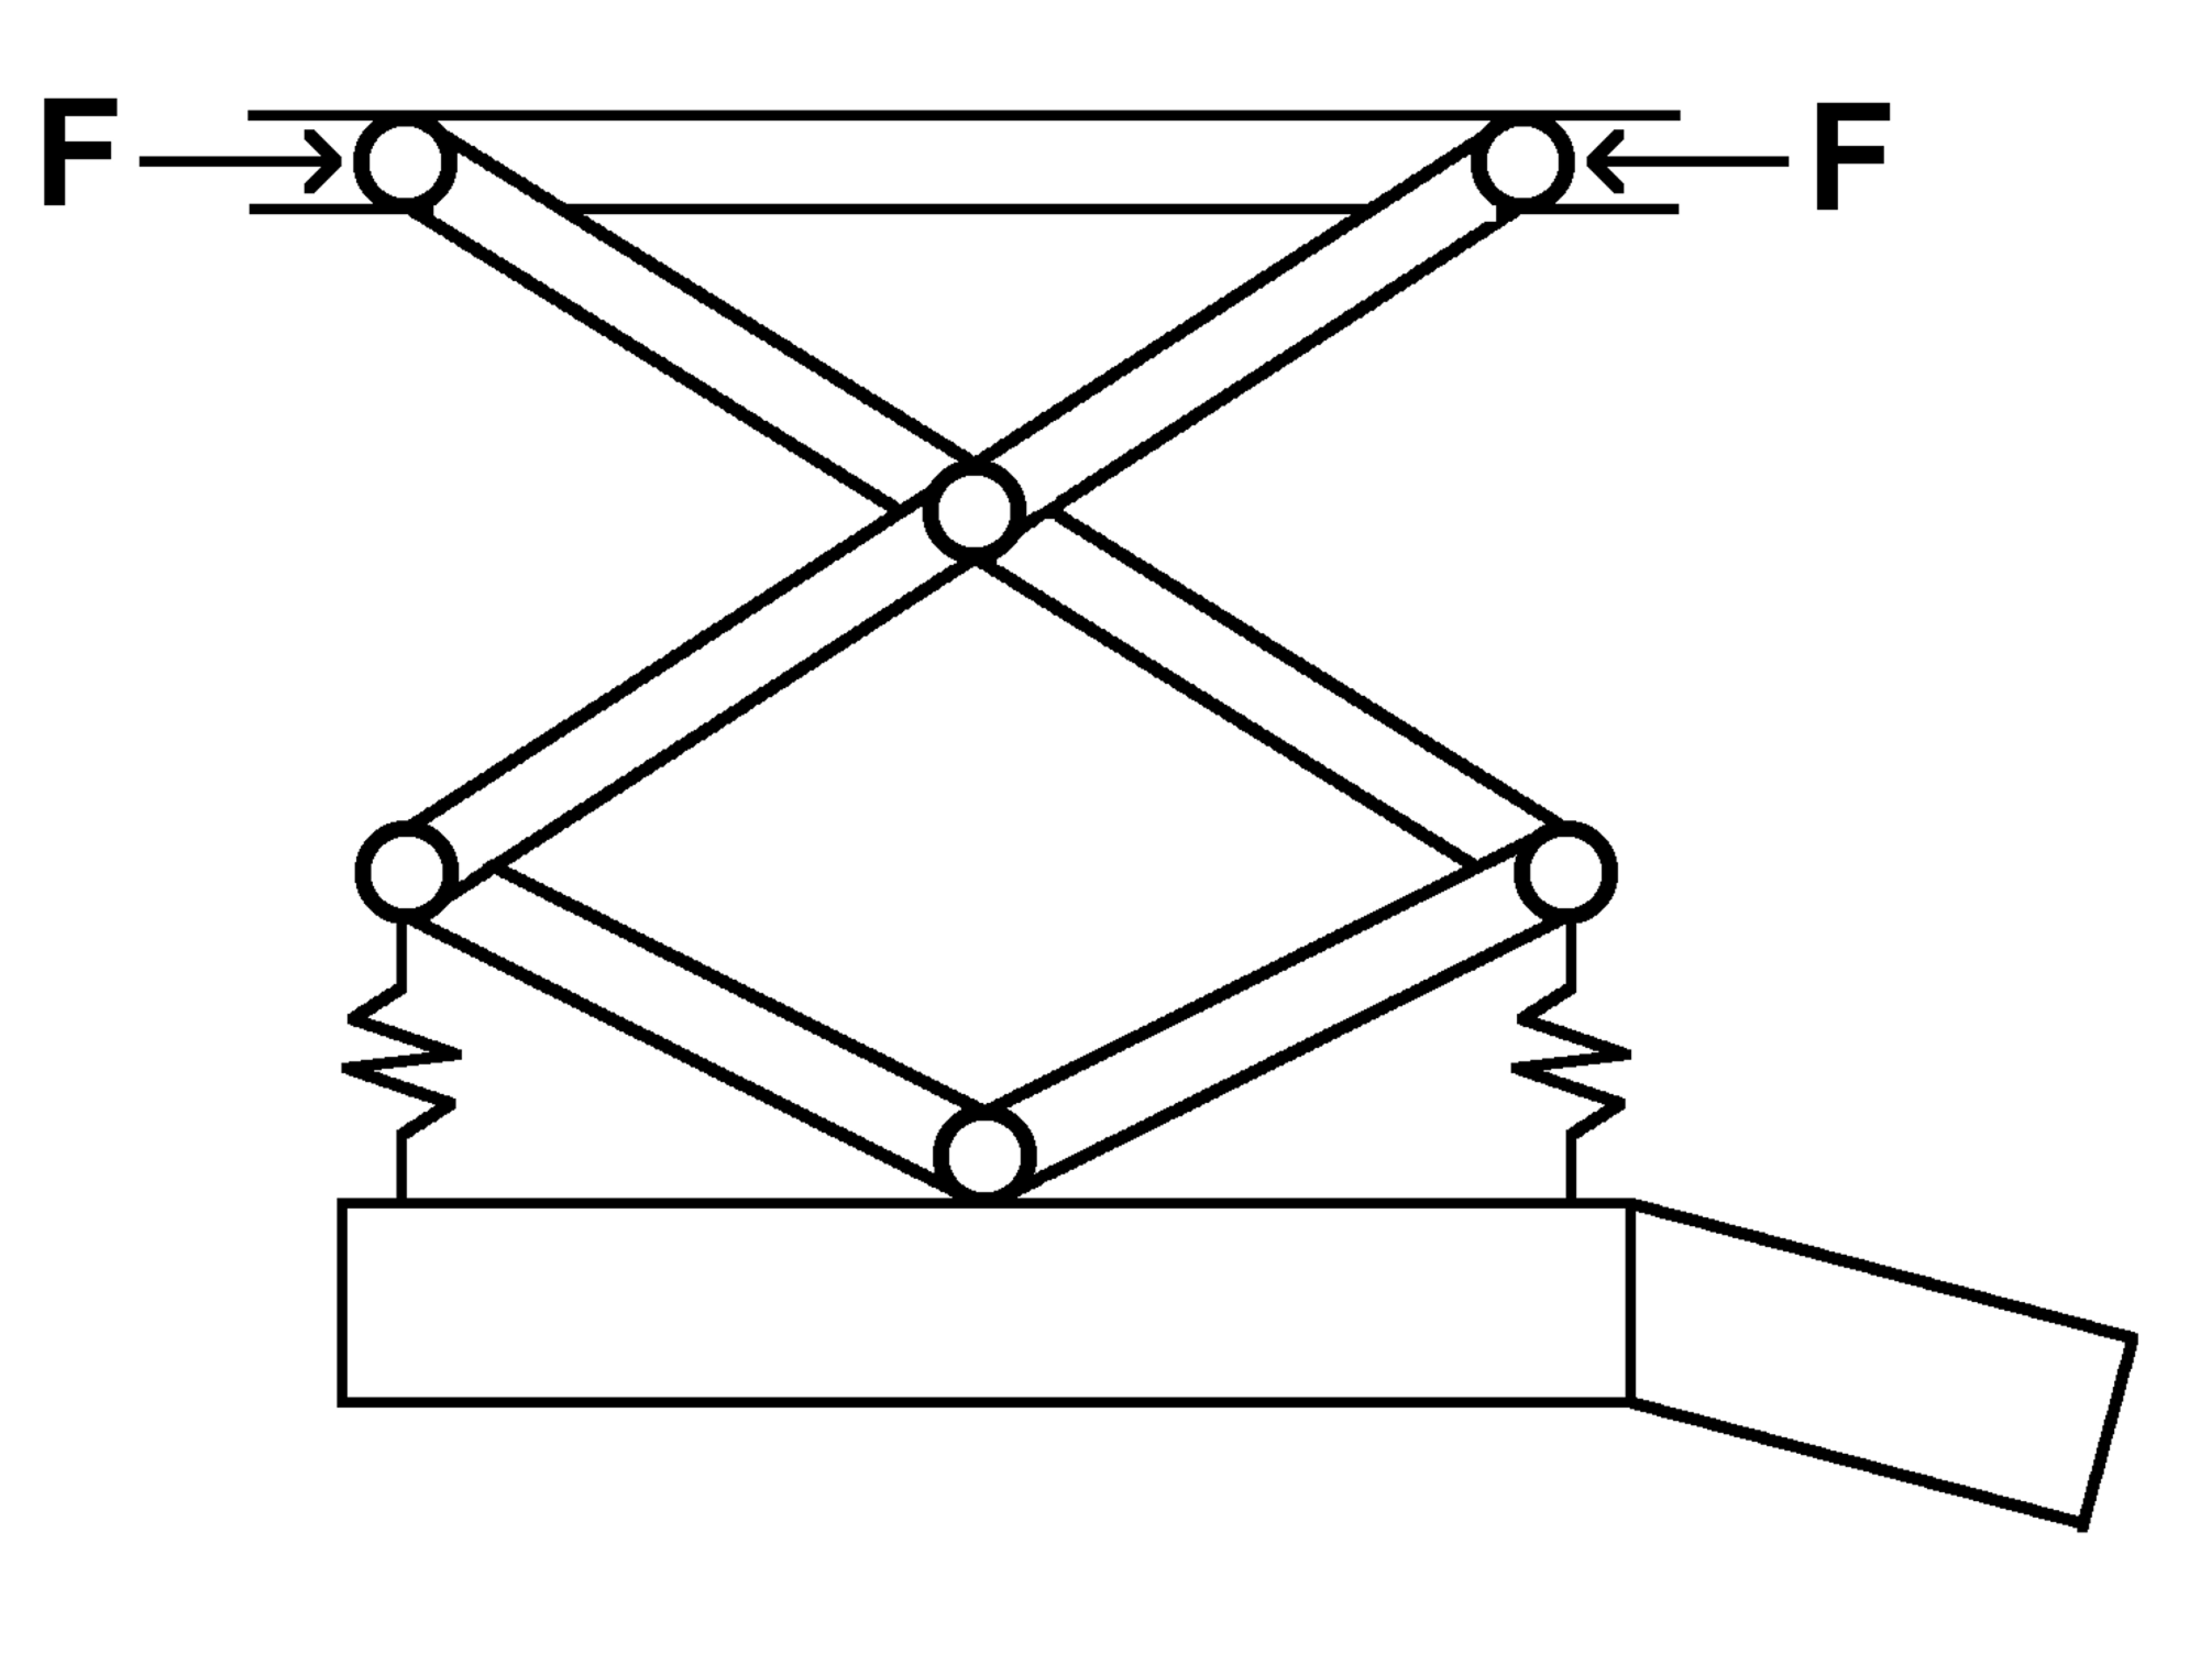
\includegraphics[height=\imageheight]{legDesign}
					\caption{Diagrammatic representation of the pantograph mechanism used for the robot's legs}
					\label{legDesign}
					\columnbreak
					
\includegraphics[height=\imageheight]{legDiagram}
					\caption{Labelled Diagram indicating angles referenced in the text}
					\label{legDiagram}
				\end{multicols}
			\end{figure}			
			\begin{figure}[h]
				\centering
				\begin{multicols}{2}
					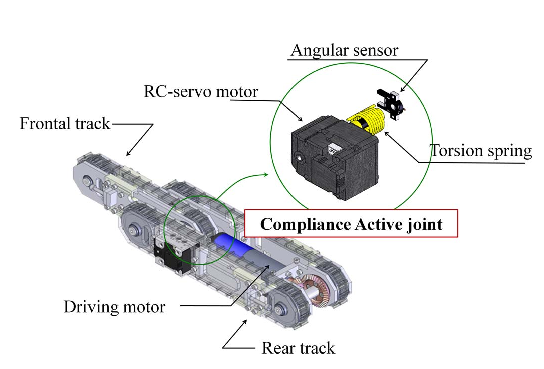
\includegraphics[height=\imageheight]{activeCompliance}
					\caption{Function and construction of an active compliance joint. Figure from \cite{park2010normal}}
					\label{activeCompliance}
					\columnbreak
					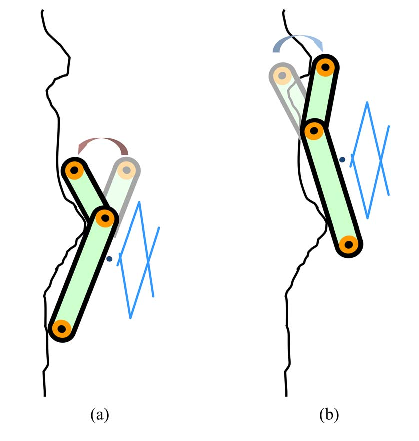
\includegraphics[height=\imageheight]{unevenBehaviour}
					\caption{Behaviour of active compliance joint over uneven surfaces (travelling upwards). Figure from \cite{park2010normal}}
					\label{unevenBehaviour}
				\end{multicols}
			\end{figure}
			\\
			The rotation of the two base legs relative to the body of the robot occurs using a motor to drive each end of the rotation mechanism.
			The motor drives the sun gears of two planetary gear systems, shown in \figref{planetaryDrive},which rotate in opposite direction so the legs move symmetrically.
			The direction is reversed for the further planetary drive system using a small differential gearbox, shown in \figref{diffGearbox}, which allows for compact reversal of motion.
			These allow the legs to move around the body, from almost directly below the robot to in a horizontal plane at $90^\circ$ to the top leg.
			As both legs are driven from the same motor at each end, both legs are symmetrical about the vertical leg at all times, and the leg position can be summarised by a single leg rotation angle $\lambda$, measured from the top leg, which varies from $\lambda = 90^\circ$ to $\lambda = 160^\circ$.
			The rotation allows the robot to adapt to different angles of the pipe more easily, as it will be quicker to drive along horizontal pipes with the almost vertical drive system, whereas vertical pipes require a more even distribution of contact points for optimal behaviour, probably requiring an angle of $\lambda = 120^\circ$ for the most even distribution of contact points.
									
			\begin{figure}[h]
				\centering
				\begin{multicols}{2}
					\includegraphics[height=\imageheight]{planetaryDrive}
					\caption{Planetary drive used to move the legs relative to the main body}
					\label{planetaryDrive}
					\columnbreak
					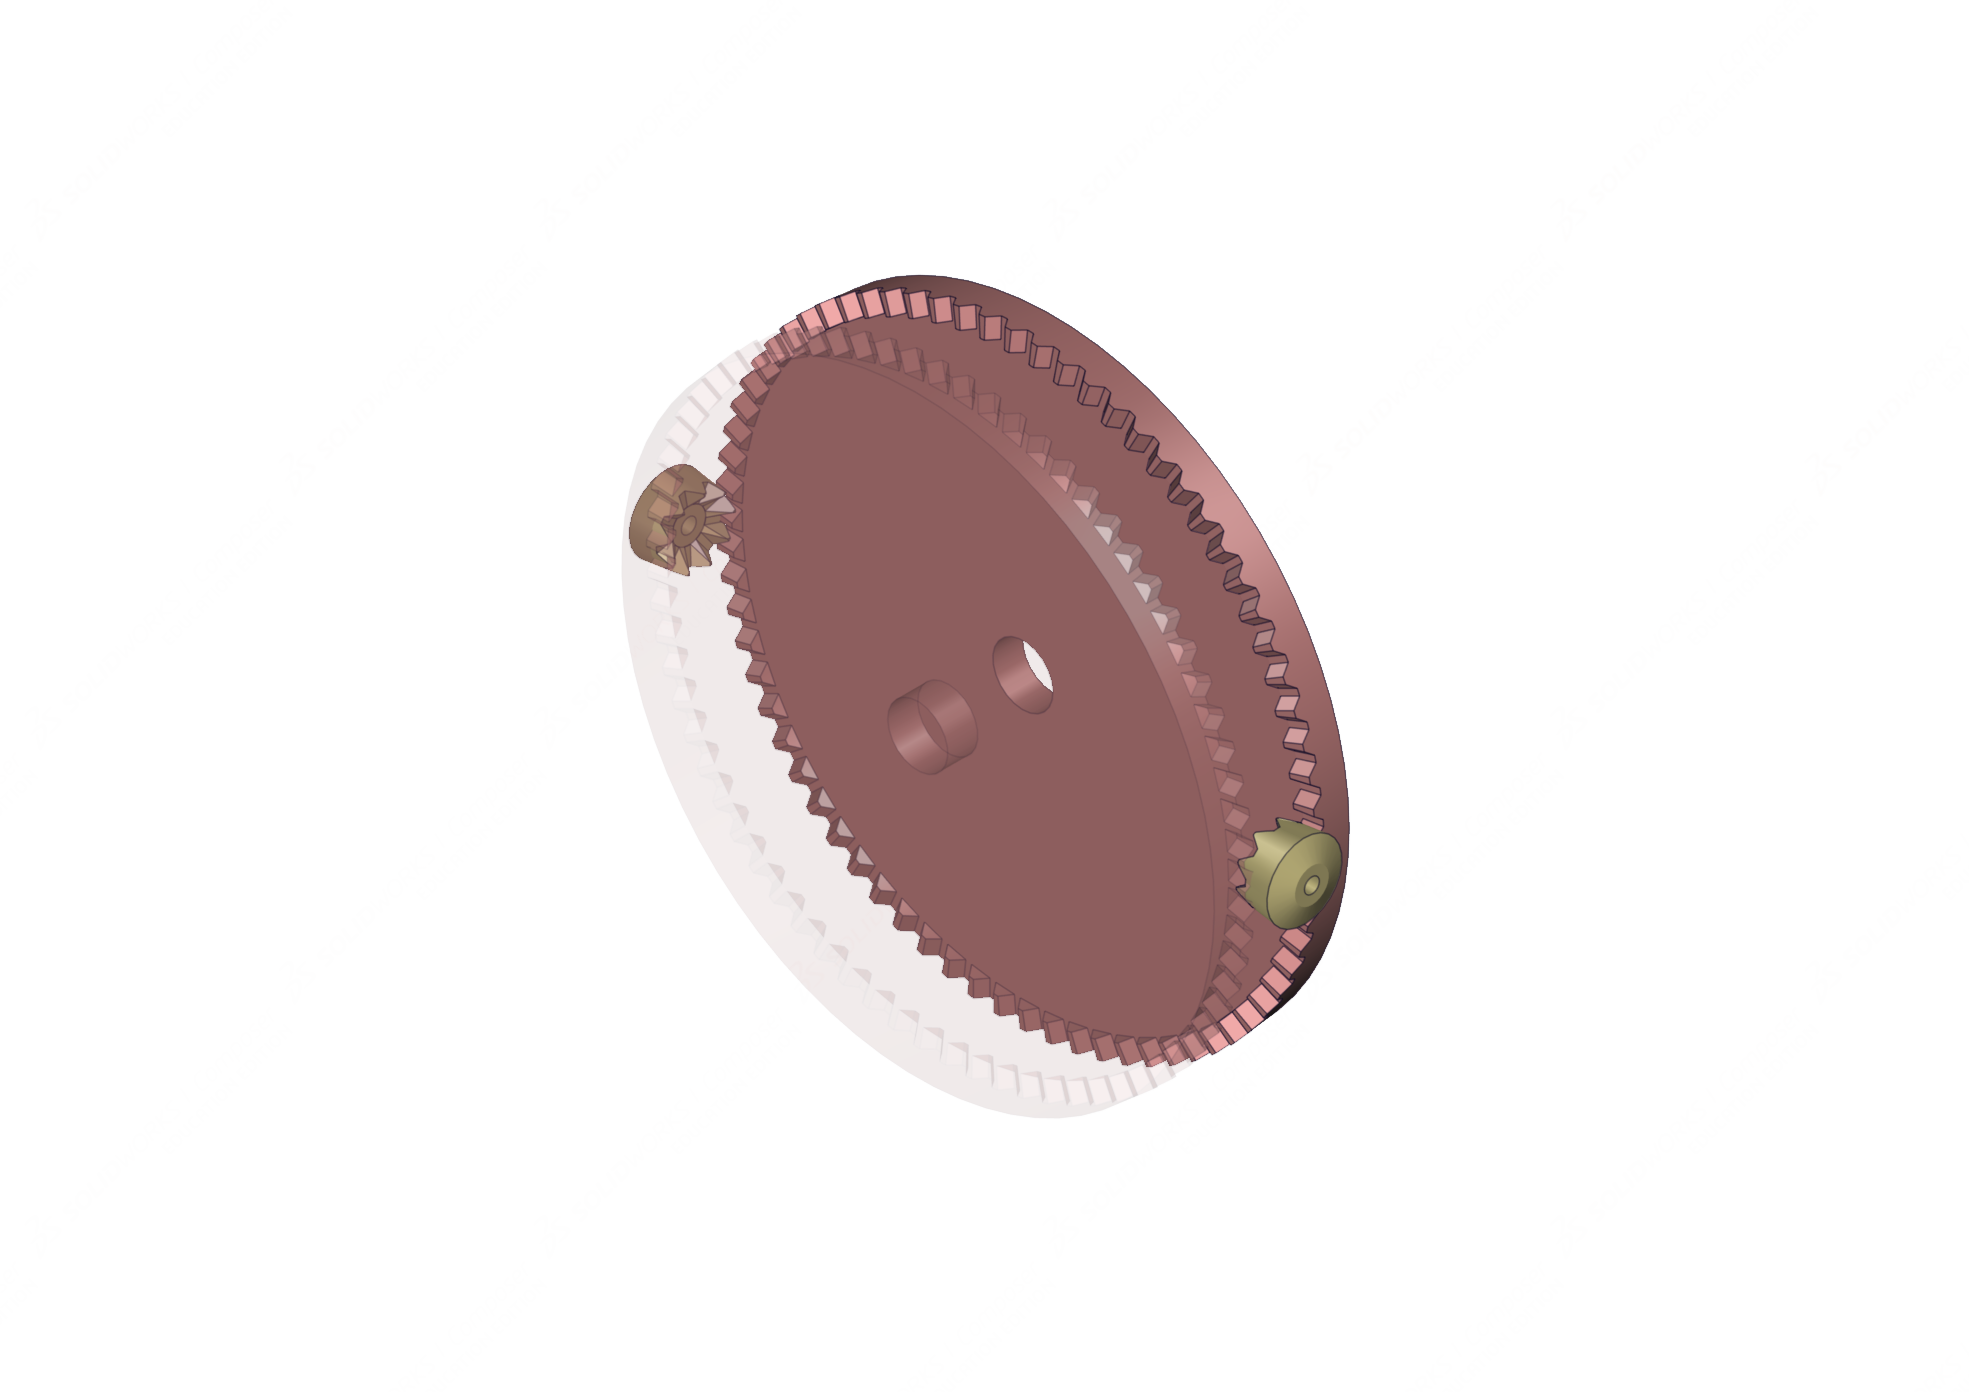
\includegraphics[height=\imageheight]{diffGearbox}
					\caption{Differential gearbox for coaxial rotational direction reversing}
					\label{diffGearbox}
				\end{multicols}
			\end{figure}
			
			The ratio between the longer base links of the pantograph and then shorter tip links is $2:1$, which gives the greatest range of diameters for the smallest change in the base distance\supercite{okada1987mogrer}, to calculate the required link length $L$ to allow the robot to adapt to the chosen range of diameters, $457.2 - 914.4$ mm.
			The pantograph angles are shown in \figref{legDiagram}, which results in:
			
			\begin{align}
				r_{min} &= \frac{3L}{2} \sin \left( \theta_{min} \right)
				\\
				r_{max} &= \frac{3L}{2} \sin \left( \theta_{max} \right)
				\\
				\implies \Delta r &= \frac{3L}{2} \left( \sin \left( \theta_{max} \right) - \sin \left( \theta_{min} \right) \right)
				\\
				L &= \frac{2 \Delta r}{3 \left( \sin \left( \theta_{max} \right) - \sin \left( \theta_{min} \right) \right)}
			\end{align}
			
			Assuming the pantograph will ideally move from an angle of $\theta_{min} = 10^\circ$ to $\theta_{max} = 60^\circ$, spanning a change in radius of $228.6$ mm, $L = 220.1$ mm, and the smallest leg radius $r_{min} = 57.3$ mm, not including the depth of the tracks.
			This means that, if the track depth is $70$ mm, the body diameter $D_r$ has a maximum of $202.5$ mm, setting a constraint on the dimensions of the inner body based on the design criteria.
			\\
			The minimum length of the body is also set by this, as it means that the body length $l_{min} = L \cos \left( \theta_{min} \right) = 216.8$ mm.
			A maximum body length can be found by considering the ability of the robot to turn corners inside the pipe, and it is necessary to consider how this compares to the minimum to make sure there is no loss of mobility.
			For the duration of this calculation, it is assumed that the robot is in the smallest possible pipe diameter $D_{pipe} = 457.2$ mm, and the curvature radius $r_c = \frac{3}{2} D_{pipe} = 685.8$ mm.
			As the robot diameter $D_r \nless \left( 2 \sin \left( 45^\circ \right) - 1 \right) D_{pipe}$ mm the maximum length can be found from the following equation\supercite{roh2005differential}:

			\begin{align}
				l_{max} &= 2 \sqrt{4D_{pipe}^2 - \left( D_{pipe} + D_r\right) ^ 2}
				\intertext{which, using the maximum $D_r = 436.4$ mm}
				l_{max} &= 1266.3 \ \mathrm{mm} \notag
			\end{align}
			% Makes max volume 187*10^6 mm^3
			Using \figref{legDiagram} to calculate the required force output of the linear actuators in order for the robot to operate at all angles.
			As such, the worse case scenario is considered, where the robot is climbing vertically and must create enough normal force for friction to support its entire weight.
			This results in:
			
			\begin{align}
				N &= \frac{2 F \tan \left( \theta \right)}{\cos \left( \phi \right)}
				\\
				F_f &= \mu_{t,p} N
				\\
				&= \frac{2 \mu_{t,p} F \tan \left( \theta \right)}{\cos \left( \phi \right)}
				\intertext{where $F_f$ is the frictional force on one track, and $\mu_{t,p}$ is the coefficient of friction between the tracks and the pipe. \newline In order for this to balance the weight W:}
				\begin{split}
					W &= 3 F_f
					\\
					&= \frac{6 \mu_{t,p} F \tan \left( \theta \right)}{\cos \left( \phi \right)} \label{maxWeight}
				\end{split}
				\\
				\implies F &= \frac{W \cos \left( \phi \right)}{6 \mu_{t,p} \tan \left( \theta \right)} \label{reqMaxNorm}
			\end{align}
			
			Since testing would be required to find the greatest angle $\phi$ that is experienced by the robot in general use, as well as an estimate for the coefficient of friction $\mu_{t,p}$, it is tricky to estimate the force required for the actuators.
			However, estimates from other papers for $\mu_{t,p}$,which are $1.21$\supercite{sato2011development} - $1.6$\supercite{park2010normal}, allow us to create a worst case estimate for the required force of $1.21$.
			From \equationref{reqMaxNorm}, it is clear that the worst case scenario occurs in straight sections, where $\phi$ is expected to be close to $0^\circ$, with the smallest pipe diameter, as this minimises $\theta$, which will require the most linear actuator force.
							
		\subsection{Power}
		
		\subsection{Sensing}
		
		\subsubsection{Rotary Sensors}
            		
            There will be rotary sensors will be placed at the connection between the legs and the tracks. 
            This will allow the robot to know the angle of the legs and therefore compute the distance to the walls and how much the legs must extend in order to produce a particular force. 
            Rotary sensors will also be placed at the top of the arms. 
            This will allow the robot to know the angle at which the arms are so that they can be rotated appropriately. 
            For this job arms magneto resistive sensors and hall effect sensors were investigated. 
            The benefits of Magneto resistive sensors are that they are highly accurate, not sensitive to noise caused by external vibrations, very small and consume little energy. 
            However they do not measure 360 rotations and can be sensitive to temperature fluctuations. 
            Meanwhile Hall effect sensors have the advantage of being able to measure 360 degrees of motion but they are not as accurate as Magneto resistive sensors. 
            Since in this application accuracy is the most important factor and 360 degrees motion is not required magneto resistive sensors will be used.
            \\
            There are three main types of magneto resistive sensors that had to be considered.
            These are anisotropic magenetoresistance sensorts (AMR), tunnel-magentoresistance sensors (TMR) and giant magnetoresistance sensors (GMR). 
            Table [] compares them. 
            MR is the magnetoresistance ratio and it describes how sensitive the sensor is to changing its electrical resistance with changes in external magnetic fields.[https://en.wikipedia.org/wiki/Magnetoresistance]
            \\
            TMR sensors are made of three layers, the ferromagnetic free layer, the insulator barrier layer and the ferromagnet pin layer [\url{https://en.wikipedia.org/wiki/Tunnel_magnetoresistance}].
            The barrier layer is an insulating material.
            The free layer changes it magnetic orientation to align with externally applied magnetic fields whilst the pin layer has its magnetic orientation in a constant direction.
            This means that when the externally applied magnetic field is aligned in parallel with the magnetic field of the pin layer there is low resistance and therefore large current, but as the external magnetic field changes direction so that it is becomes more anti-parallel to the pin layer’s magnetic field the resistance increases. 
            The changes in current that this causes can be detected. [https://ieeexplore.ieee.org/document/1003148]
            \\
            GMR sensors are very similar to TMR however the current in these flows parallel to the layers whereas in the TMR it flows perpendicularly across it.
            There is a change in resistance due to electron scattering that is dependent on the spin orientation of the atoms within the ferromagnetic layers.
            \\
            AMR sensors the other hand only have one layer of permalloy. 
            Changes in resistance in AMR sensors vary depending on the material, but largely it is due to changes in spin-dependent scattering.[  https://www.sciencedirect.com/topics/materials-science/anisotropic-magnetoresistance]
            The anisotropic effect is the dependence of resistance in the angle between the electric current and the external magnetic field.
            \\
            Between these TMR was chosen because it has less age deterioration and temperature drift that the other two. 
            This is important when the accuracy is the most important factor. 
            Further it can be seen that it has greater sensitivity which provides greater resolution. Further because it produces a high output it does not require extra amplification reducing cost and complexity. 
            
            % Insert table here

            \subsubsection{IMU vs AHRS vs INS}
            
            The robot needs to be able to determine its orientation so that it can calculate its pose. 
            This information is fed into the localisation system as well as the navigation control system. 
            Three options were considered to provide this information, an attitude heading reference system (AHRS), an inertial measurement unit (IMU) and an inertial navigation system (INS). 
            \\
            The main consideration for this is providing as accurate information as possible since the accuracy of the robots systems is highly dependent on the accuracy of its knowledge of its pose.
            The table below compares the three options.
            It was decided to use the AHRS because it provided attitude values and also suffers less drift than the IMU due to its application of a Kalman filter. 
            The INS is more expensive but can provide more accurate information if regular GNSS information is available. 
            However this is not available, therefore the extra expense would not be justified. For this reason an AHRS was chosen to be used.
            \\
            In particular the Ellipse 2 Micro AHRS was picked.
            This is because it is light and compact. It has a weight of 10g and size of 26.8 x 19.8 x 9.5 mm. [ \url{https://www.sbg-systems.com/products/ellipse-micro-series/?gclid=CjwKCAiArbv_BRA8EiwAYGs23MIy00g-YW8iNNNozsH9mjSeER1raROv2mD2hZ86wU91BhrPTuxHTBoCyocQAvD_BwE#ellipse-micro-inertial-navigation-system}]
            
            % Insert table


        \subsubsection{Odometers}
        
        Physical odometers are required to past information into the localisation system. 
        These suffer drift however, as described in the localisation section, can provide useful information to produce a more accurate overall system.
        \\
        One odometry method would be to use the relation between the motor power and track speed.
        This would have the benefit of not requiring any extra sensors. 
        It would therefore be the cheapest and least complex solution.
        However its accuracy would be too low due to the non-linear relationship between the power and the motor that would be dependent on that angle the robot is travelling, the weight of the robot, and the coefficient of friction between the robot and ground, among other things, all of which would vary.
        For this reason this method would not be used.
        \\
        Wheel rotary encoders are another solution that is reasonably uncomplex and cheap.
        The use of the robots clock and $s=ut$ would allow the displacement to be calculated. 
        Such a method does incur errors such as the tracks slipping which can lead to odometer drift.
        \\
        For these odometers there was the option of using encoders or resolvers.
        Resolvers were discounted due to their complexity and lower speed range.
        For the encoders there was an option to use relative or absolute encoders. 
        Absolute encoders were found to not be required since it is only the relative shaft position that would need to be measured.
        \\
        There were three main types of encoders to consider: magnetic, optical and capacitive.
        Magnetic encoders have the advantage of being more robust and not as sensitive to environmental contamination as optical sensors.
        However, they are often not as accurate. 
        Further, they can suffer interference from electrical motors and since the electrical motors in the tracks will in close proximity to the encoders this would be a significant factor. 
        Optical encoders have a much higher accuracy. 
        However, they consumer more power and are more likely to break. 
        The LEDs in encoders can burn out after 10,000 to 20,000 hours of use. [https://www.machinedesign.com/automation-iiot/article/21833929/capacitive-encoders-deliver-durability-and-precision]
        Since the effectiveness of the localisation is highly affected by  the effectiveness of its odometers, this risk of failure of the odometer has high significance.
        \\
        Capacitive encoders have greater robustness, and do not consume as much power due to not using an LED. 
        They required 6 to 10mA of current compared to 20 to 50mA required by optical encoders.
        Capacitive encoders are also more compact than optical and magnetic encoders and are less expensive [https://www.machinedesign.com/automation-iiot/article/21833929/capacitive-encoders-deliver-durability-and-precision]. 
        They have a downside of being prone to electrical interference however modern packages housing the encoders tend to make this less significant than the noise that the other encoders face. [https://www.machinedesign.com/automation-iiot/article/21833929/capacitive-encoders-deliver-durability-and-precision]
        \\
        The table below compares the metrics that it need to be considered when choosing which type to use. 
        Due to the relative inexpense of these compared to other parts of the robot it was not considered to be a factor worth considering. 
        From this decision matrix it was decided to use a capacitive odometer. 
        In particular the Murata electronics’ capacitive encoder will be used. 
        On an order of 1000 the unit price is £0.694. 
        It has an operating range of -49 to 85C.

        \subsubsection{Sensing pipe damage}
        
        For the robot to provide value to its users it must be able to identify several features within the pipes. 
        Firstly it must be able damage so that it can be determined whether the pipes need to be replaced.
        The robot will be primarily used on cast iron pipes. 
        Corrosion and cracks are the major categories of damage that can be found within these pipes.    
        Secondly, the robot can be used to provide information about the location connecting pipes, joints, valves and other objects within the pipes.
        \\
        In order to determine how to detect the damage features 3 main steps were used. 
        Firstly determining the type of sensor to use and therefore the type of data that will be processed. 
        Secondly having determined the type of sensor looking into the best types of that type of sensor. 
        Thirdly investigating how to best process the data provided by the sensor so as to extract the desired information.
        
        \textbf{Constraints to consider}
        
        When assessing the type of sensor the constraints of the application as well as the desired outcomes must be considered. 
        The robot would be involved in inspecting pipes of varying diameters, they may vary as the robot goes along the pipe as well as in different locations. 
        Therefore the detection systems must be able to adapt to different diameter pipes. 
        Secondly, it is important to maximise the amount of valuable information that can be gained from an excursion since a large amount of investment goes into providing the robot with access to the pipes.
        Further since in some places it is disruptive to provide access to the pipes and the cost of doing so is a function of time, it is important to use a method that allows the robot to move relatively quickly through the pipes. 
        Thirdly, the robot should be able to adapt to pipes of different materials since although the main use case will be in cast-iron pipes it could also be applied in steel pipes or PE pipes.

        \textbf{Type of sensors}
        
        Magnetic Flux Leakage inline inspection tools is an array of sensor placed in a circular configuration. 
        The arrays have magnets which produce a magnetic that flows through the pipes between the poles of each of the arrays. 
        Damage in the pipe wall leads to variation in the flow of flux. 
        A flux sensor is placed between the poles of the magnets and detects this variation which it uses to determine if there is damage present. 
        The flux increases in pipe for tensile stresses and decrease for compressive stresses.
        \\
        This type of detection is beneficial because it can detect stresses in the material which might predict damage in the future.
        Further, it allows damage within the pipe walls to be detected. 
        It is also less sensitive surface condition compared to ultrasonic which is useful when considering that there may be dirt build up on the walls.
        \\
        However, the MFL requires a constant gap between it and the sides of the walls and this gap needs to be small find the exact numbers. 
        In order to get around this problem it was considered designing a mechanism which had the detectors on extendable arms which extended outwards in order to adapt to the pipe diameter. 
        However, this technique would mean in larger pipe diameters there would be less resolution. 
        What’s more the circular geometry meant gave the mechanism an added complexity which would introduce greater cost and weight to the robot. 
        What’s more the requirement to have an array of magnets would have considerably increased the weight of the robot get data on the weights of mfls. 
        Another negative is that corrosion products can build up on the magnets which decreases its accuracy. It was therefore decided not to use an MFL.
        \\
        Piezoceramic Ultrasonic Transducer Detection is a method that measure the time it takes for an emitted ultrasonic pulse to return to the sensor having reflected off a medium boundary. 
        This sensor is usually a piezoceramic transducer.
        By using short pulses internal flaws of the pipe can be detected.
        It can detect these flaws at greater depths into the wall than MFL.  
        Further it can detect these flaws to a greater degree of accuracy than the MFL technique.  % Find data for this claim. 
        However, most UT techniques require a couplant fluid between the sensor and the wall. 
        This would make it difficult to adapt to different diameters and would require the robot to be supplied with a fluid, something that would reduce its range considerably.
        Further, it would not be desired to introduce a foreign fluid into live gas pipes. 
        On top of this it needs to be calibrated with the thickness of the pipe. 
        In a pipe system in which there is imperfect information and the pipe thickness changes as the diameter changes this would not be feasible. 
        Therefore Ultrasound Detection was decided against.
        \\
        Eddy Current Testing (ECT) uses a probe that produces an alternating magnetic field using an electromagnet.
        This induces an eddy current in the side of the pipe. 
        The eddy current is then measured and an algorithm can from this information produce information about any cracks that it has passed over. 
        This has an advantage over MFL because it can be used in both ferromagnetic and non-ferromagnetic material for surface inspection, however for tubing inspection it cannot be used for ferromagnetic material which would therefore not be useful when inspecting cast iron pipes.
        The ECT  also has the benefit of being non-contact.
        On the other hand ECT is more sensitive to differing permeability of the wall when compared to MFL and the data is therefore harder to interpret. % Get source. 
        Beside this ECT is another technique which requires the sensor to be in close proximity to the wall which would make it hard to adapt to different diameters. 
        For these reasons it was decided against.
        \\
        A innovative technique that is being developed for use in live pipe conditions involves the robot carrying a heater and a IR camera. 
        When there is a crack in the gas pipe the acceleration of the gas through the crack which creates friction causes temperature changes to the gas that can be detected by the IR camera. 
        This technique has the benefits of not requiring sophisticated computer vision as well as being able to work for many different diameters. 
        However its downside is that it can only detect through cracks thus meaning reducing the value that it can provide to a consumer. 
        \\
        Electro Magnetic Acoustic Transducers (EMAT) are a non-contact ultrasonic testing technique that does not require a couplant. 
        The EMAT works by using magnetic fields to induce ultrasonic waves into the wall of the pipe.
        The waves that go through the pipewall when they return induce a current in the EMAT’s receiving coil.
        EMATs can be used to provide information about the thickness of the wall and wall loss due to damage such as corrosion. 
        The fact that it can provide information about defects within the walls of the pipe and that gas distribution companies already know how to use EMAT data is their risk models means that it has a major advantage. 
        The downside is that on the robot it will only be able to be deployed at certain angles and will miss out on damage over the majority of the circumference of the pipe. 
        For this reason it  cannot be used alone.
		\\
        Visual sensing using computer vision techniques to visually identify with a camera damage to the interior of the pipe. 
        This has the benefit that the information produced is to interpret and the data collection can occur at a faster pace. % Get data 
        Further the camera equipment required for it is relatively uncomplex and inexpensive and would be required for the navigation of the robot anyway. 
        Further visual detection can be used with a wide range of diameters since the camera does not need to be in close proximity with the wall. 
        Further it can be used with any pipe material. 
        The downsides is that it is has lower precision. Further, its ability to accurately detect damage can be affected by lighting conditions and build up of dirt on the surface of the pipes. 
        On top of that it cannot detect internal defects in the pipe. % get data to show that this does not matter. 
        Despite this, its adaptability to the different pipe environments meant that this would be taken forward for further consideration.
        \\
        A laser scanner provides higher resolution information about the inner surface of pipes. % Give a resolution number 
        It allows the depth of pits and cracks to be determined and the integrity of different sections of the pipe. 
        From this information a laser scanner allows the company to know how much material is left, what the remaining life of the asset is and what the risk of leakage is.  
        These can be used for a range of pipe diameters so are therefore adaptable. The downside of laser scanners compared to visual sensing is that it is a slow process to acquire detailed high-resolution information. 
        For a 1 metre diameter pipe it was calculated the robot would need to stop every 0.37m and carry out a 360 degree scan that takes 6 minutes. 
        This scan covers 0.466m along the axis of the pipe. 
        This means that the average rate when the laser function is activated is 6.1cm of pipe length per minute. 
        This calculation was made using data from 2grobotics. [  https://www.2grobotics.com/laser-scanning-crawler-integration-for-internal-pipe-inspection/]
        \\
        The laser scanner therefore offers major advantages for providing more detailed information about the pipes than visual sensing. 
        However, because of its speed of acquiring data it cannot be used all the time if a large distance of pipe needs to be inspected.
        \\
        Ideally metrics would be looked at to determine the accuracy of these techniques in the environment that the robot would be in. 
        This would involve looking at false poistives, false negatives, recall and precision.
        However, since the robot is not constructed and there is currently no access to these environments this would not be possible.
        \\
        It has been decided that the robot would use a combination of laser scanning, visual detection and EMATs.
        The visual detection would allow the robot to move more quickly through the pipe where there is not any damage, saving time and providing extra range. 
        The EMAT can be deployed when that data is desired by the gas distribution company in order to form risk models. 
        Once the visual system detects damage  above a certain threshold it activates the laser scanner to extract greater resolution data about the damage. 
        This threshold will be decided after test runs are done with the partnered company and will be adapted based on the difference risk preferences of the different clients.
    	\\
        \textbf{Constraints imposed on the rest of the robot by the visual detection system}
        The visual detection system provides constraints on the processing of images. The FPS of the camera chosen is 40.
        The robot is moving along at $0.1ms^-1$. 
        Therefore to detect provide a detection every 1cm the robot must be able to process images at 10 FPS.
        \\
        Firstly the inverse of the computation time for one frame would need to be less than frame rate otherwise there would be a backlog of images, which would require a large memory saving device prior to the processing of the images. 
        In case some images do occasionally take longer to be processed than the frame rate there is a small amount of memory allocated to saving the pre-processed images. 
        This uses a first in first out system.

		\subsection[Communications]{Communications - Louis Emanuel}

		Communication is an important capability for the autonomous robot as in order to operate it safely and efficiently, it's critical to know the whereabouts of the robot within the pipe at any given time. 
		An additional and more complex requirement is also the ability for bidirectional communication so the robot can be updated on its position and given instructions when necessary. 
		\\
	    The difficulty arises in finding a suitable communication method that is capable of operating in the difficult pipeline environment. 
	    With pipe bends, thick steel walls, metres of soil, and noise interference, the choice of communication must be able to overcome these barriers without inhibiting locomotion. 
	    \figref{commsTable} outlines several communication methods which have been widely practiced in the Oil and Gas industry\supercite{acoustic2020}.
	    \\
	    
        \begin{figure}[h]
			\centering
			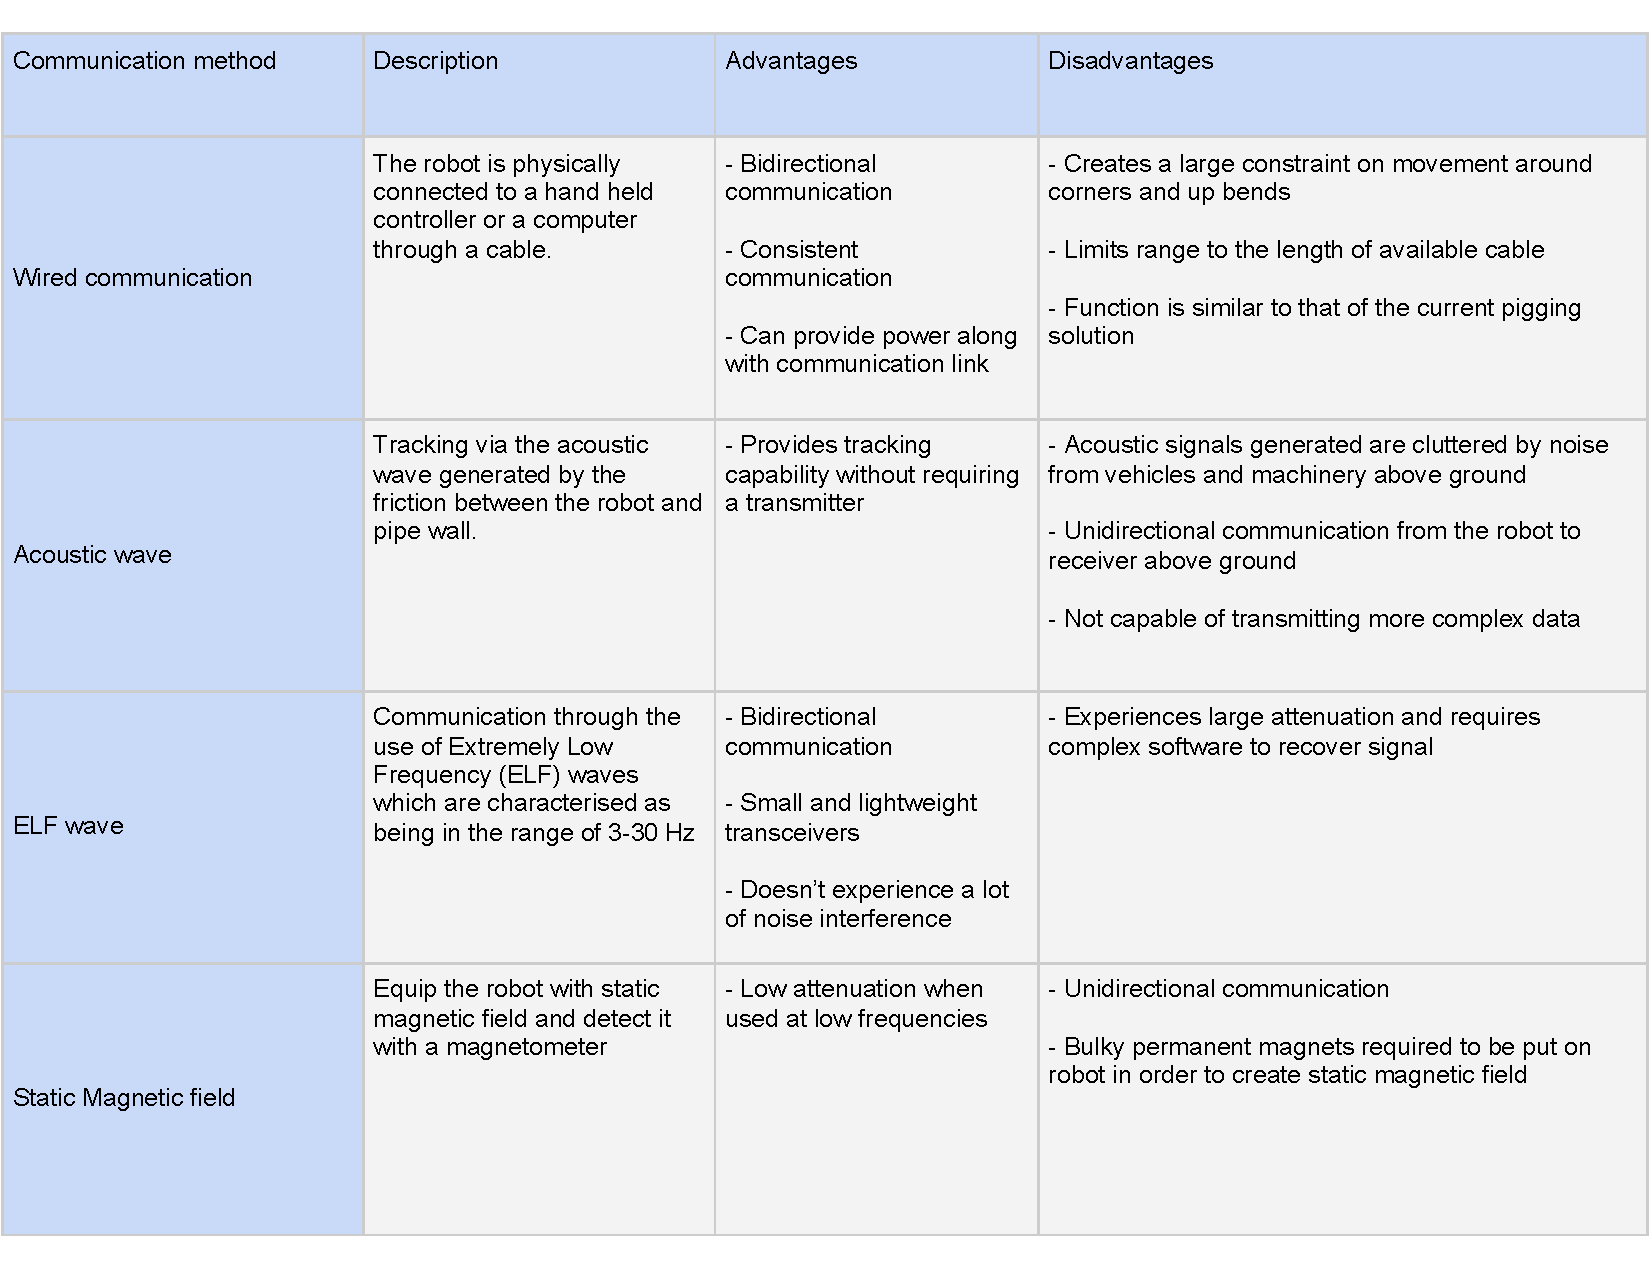
\includegraphics[scale=0.6]{commstable.pdf}
			\caption{Communications Comparison}
			\label{commsTable}
		\end{figure}
     	A critical requirement of the robot is for it to have a real time understanding of its location in order to navigate pipes and localise pipe damage. 
     	From the solutions in \figref{commsTable}, the only methods capable of this are ELF and wiring. 
     	However, ELF communications requires a significantly sized receiver\supercite{elfreceiversize} which is infeasible to house in the robot without inhibiting speed, locomotion and range. 
     	Consequently, for feeding data to the robot, a wire will be used.
        \\ 
        \hspace*{3ex}Although a wire allows bidirectional communication, it is incapable of determining the position of the robot. 
        Therefore, a method of communicating with surface receivers must be used in order to determine its position. 
        Given the size constraints and interference challenges, acoustic and magnetic methods are unsuitable for this application. 
        Instead, ELF communication is used which with present technology is capable of travelling through up to 20m of soil. 
        This allows location to be determined, and fed back to the robot through the wiring in order to compensate for the the accumulated locating error generated in the on board INS.
         
        $\textbf{Communication Map}$
        
        \begin{figure}[h]
			\centering
			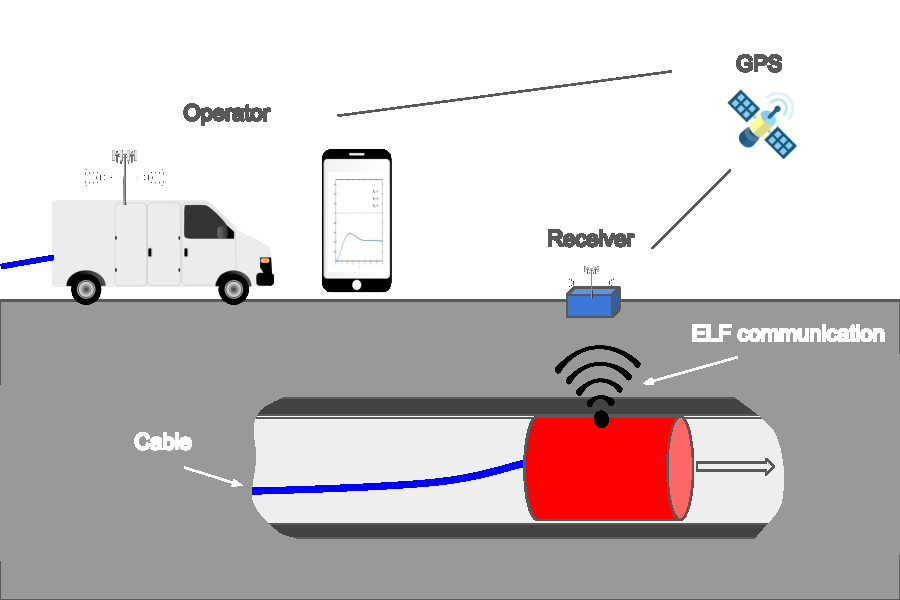
\includegraphics[scale=1]{comms layout.pdf}
			\caption{Communications layout} % This needs a citation for the source I think
			\label{commsLayout}
		\end{figure}
        
        \figref{commsLayout} provides an overview of the communication architecture. 
        Starting from the operator, an optical fibre which is capable of bidirectional communication is fed down to the robot by an automatic cable reel. 
        On board the robot is an ELF transmitter which pulses ELF waves at 22Hz to to the receivers above ground. 
        These receivers then calculate the global position of the robot, and feed it back down to the robot via the optical fibre.
       
        \textbf{Wired connection}
        \\
        The wired communication line presents a challenge for the locomotion of the robot. 
        In order to satisfy the communication requirements, it must deliver data at a suitable rate without creating a hindrance to locomotion along the pipe and around corners. 
        The proposed solution uses a Kevlar lined wire with an optical fibre. 
        Through making assumptions on a constant frictional coefficient throughout the pipe and steady speed, we arrive at the following initial equation for drag. 
        \begin{align}
				F_0 = \mu_g L_{wire}   g \rho
		\end{align}
        
        % Not sure about this value of F0
        
        Where $L_{wire}$ is the length of wire at current time, $\mu_g$ is the coefficient of friction between the cable and ground and $\rho$ is the mass per unit length of the cable.
        
        This equation is very simple and does not take into account the corners the robot is designed to navigate. 
        Therefore, through modelling corners as segments of a cylinder, we can justify the use of the capstan equation [x] which describes the resistance to sliding of a flexible but inextensible cord wrapped around a cylinder. 
        For a series of corners, the following equation is derived.
        \begin{align}
                F_D = F_0 \boldsymbol{\cdot} {e}^{\mu_c \sum \alpha} \label{cableDrag}
        \end{align}

		Where $\mu_c$ is the coefficient of friction between the cable and corners and $\alpha$ is the angle swept by the cable around the cylinder in radians. 
	    Hence, in order to minimise this drag force, a solution must be found that satisfies the bandwidth capabilities whilst minimising the mass per length and friction coefficients.  
	    In this case, a Fiber optic cable is better in almost every sense over alternatives. 
	    For example, a typical fiber cable weighs 4Lbs/1000ft, requires a power of 2W and is immune to noise. 
	    In comparison, the next best alternative is copper wire which weighs 36Lbs/1000ft, requires >10W of power and is susceptible to EM interference [x].
	    \\
	    Finally, in order to minimise friction coefficients and absorb the large tensile strength in the wire, a protective coating must be applied to the cable. 
	    This technology is widely developed with smoothed Kevlar reinforced cable offering a low friction coefficient whilst resisting tensile strengths up to 2800MPa [x]. For the case of a 5mm Kevlar reinforced optical fibre cable, a breaking force of 54kN can be achieved. 
	    Considering an upper estimate of \equationref{cableDrag} using $\mu$ = 0.2 [x] L = 500m $\rho$ = 0.04 $Kgm^-1$ [x] $\sum \alpha = 10\pi/2$, a tensile force of $F_D$ = 907N is estimated which is well below maximum. 
	    
	    \textbf{Automatic Cable Reel}

        From \equationref{cableDrag}, it is demonstrated that the drag force on the robot is directly proportional to the length of wire. 
        Therefore, a requirement for the reel is for it to supply the minimum amount of wire without introducing significant tension. 
        Further, the reel must be capable of self winding when the robot makes its return journey, otherwise it will impede it.
        \\ 
        \hspace*{3ex}Fortunately there are established solutions which provide this capability. 
        The automatic cable reels offered by Minicam and IPEK both offer motorised winding which is specialised for robot pipe inspection. 
        \figref{comparisonReels} compares the weight, size, power consumption and cost of each solution. 
        The MiniCam ACR 500 is chosen as it is lighter and smaller. 

        %%%INSERT QUOTE PRICE
        
        \begin{figure}[h]
			\centering
			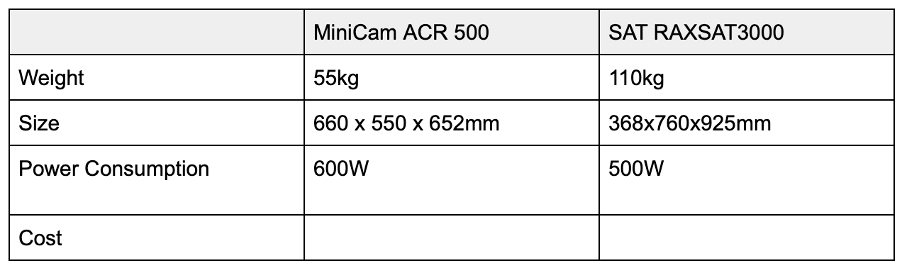
\includegraphics[scale=1]{cablereel.png}
			\caption{Comparison of Existing Cable Reel solutions}
			\label{comparisonReels}
		\end{figure}
        
        \textbf{ELF transmitter}
        
        In the system, the robot is located using the magnetic field generated by the ELF electromagnetic emitter. 
        The emitter consists of a signal generator, Ni–Zn magnetic core, power amplifier and an emitting winding in order to create the resonant frequency. 
        Also, the emitting coil is divided into two equal parts in parallel connection. 
        This method is helpful for improving the emitting power and reducing the power consumption. 
        \\
        \hspace*{3ex}The structure of the emitter is shown below. 
        As a precautionary measure, on board batteries are also included in the transmitter to ensure that in the case of a wire and robot breakdown, the robot can still be recovered. 
                
        
         \begin{figure}[h]
			\centering
			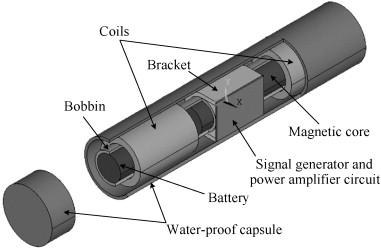
\includegraphics[scale=0.7]{ELFtransmitter.jpg}
			\caption{ELF Transmitter Structure} % This needs a citation for the source I think
			\label{ELF transmitter}
		\end{figure}
		
		
		
		\textbf{ELF Receiver}\\
		The receivers above ground are excited by the ELF electromagnetic induction. Each receiver consists of an array of sensors, batteries, GPS and 5G cellular communication. The array of sensors is used for localisation purposes, this allows the position of the pipe to be determined. The sensors are also mounted with a signal processing unit which features a filtering unit whose purpose is to discern the emitted ELF signal from background noise. The onboard GPS is necessary in order to determine the global position of the robot once it has been located via the localisation algorithm. Also equipped is a 5G cellular communication antenna. This allows the calculated position coordinates to be transmitted to the pipe entrance where it can be sent down to the robot.  Finally, the onboard batteries ensure the receivers are portable. The receiver block diagram is show in \figref{ELFrec}.
	    
	    \begin{figure}[h]
			\centering
			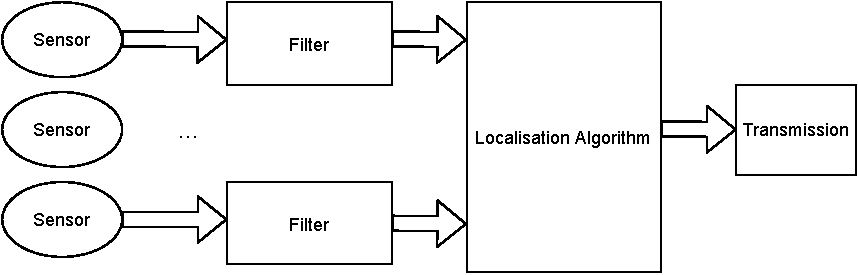
\includegraphics[scale=0.7]{blockreceiever.pdf}
			\caption{ELF Receiver Block Diagram}
			\label{ELFrec}
		\end{figure}
		

		
		
		

		\subsection{External Hardware}
		
		% Launch Tube
		
		% Beacons - maybe comms?
	
		\subsection{Materials \& Construction}
		
		% TBD after 14/2/21 - needs pressure force calcs etc
	
	\section{Product Software - ENG}
		
		\subsection[Inclination Detection]{Inclination Detection - Jim Laney}
		
		The robot is able to detect the inclination of the pipe it is in for calculation of the required leg force, as well as to aid in the mapping of the pipe.
		While the AHRS can give the angle of the robot relative to the wider world, it is not guaranteed that the robot body is parallel to the pipe.
		As such, the angle between the pipe and the robot needs to be accounted for in order to correctly measure the pipe angle.
		\\
		\begin{figure}[h]
			\centering
			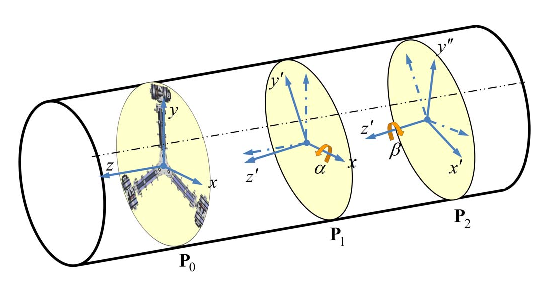
\includegraphics[height=\imageheight]{pipeOrientation}
			\caption{Angles used for calculation of pipe angle. Figure from \cite{park2010normal}}
			\label{pipeOrientation}
		\end{figure}
		\begin{figure}[h]
			\centering
			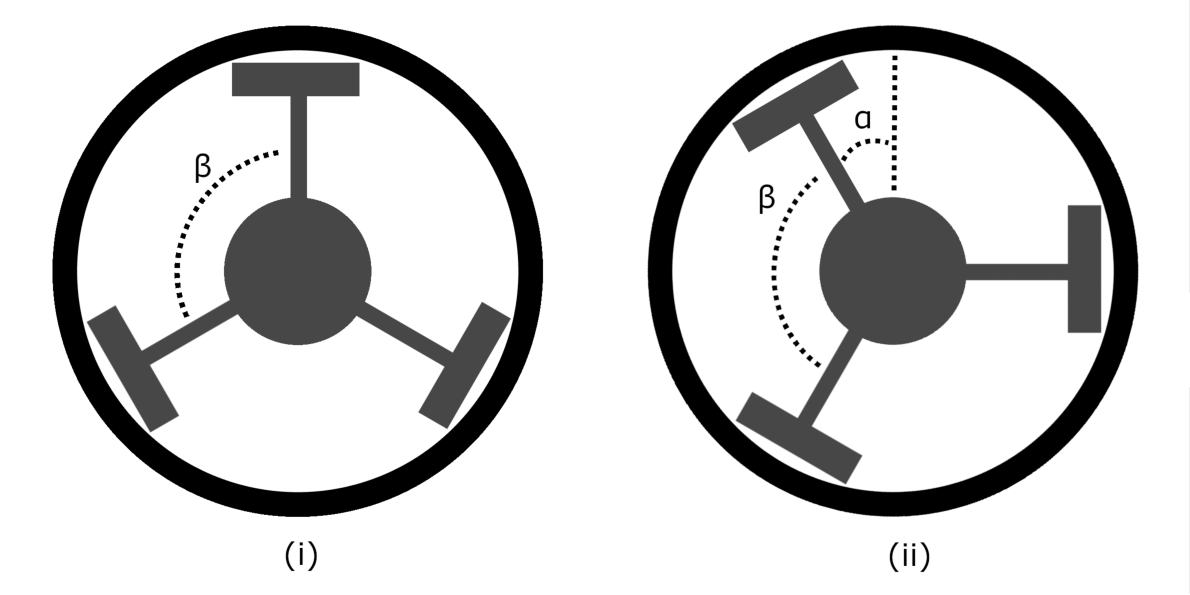
\includegraphics[height=\imageheight]{pipeAngle}
			\caption{Position of the robot within the pipe. (i) Within a horizontal or vertical bend, (ii) Within a bend at angle $\xi$ to the vertical, view shown relative to the bend rather than relative to the outside world}
			\label{pipeAngle}
		\end{figure}
		As in \figref{pipeOrientation}, the angle of the robot within the pipe can be decomposed into two orthogonal rotations, of $\alpha$ about the pipe diameter, and then $\beta$ about the robot centre, shown as $z'$ in the figure.
		Since the angle of the top leg, $\phi_T$, is $\alpha$ on the $y'$ axis ($\beta = 0$), but zero on the x axis ($\beta = 90^\circ$), the angle can be estimated using:
		\begin{align}
			\phi_T &= \cos \left( \beta \right) \alpha
			\\
			\phi_L &= \cos \left( \beta + \lambda \right) \alpha
			\intertext{where $\lambda$ is the leg rotation angle as shown in \figref{pipeAngle}:}
			\frac{\phi_L}{\phi_T} &= \frac{\cos \left( \beta + \lambda \right)}{\cos \left( \beta \right)}
			\\
			\beta &= \tan^{-1} \left( \frac{1}{ \sin \left( \lambda \right)} \left( \frac{\phi_L}{\phi_T} + \cos \left( \lambda \right) \right) \right)
			\\
			\alpha &= \frac{\phi_T}{\cos \left( \beta \right)}
		\end{align}
		Once the individual rotations of the robot are found, they can combine this with the AHRS data to find the pipe angle relative to the outside world.
		\\
		Working in 3D space, the AHRS returns rotations in a matrix $\mathbf{R}_{R,W}$, which gives the angle of the robot relative to the world.
		In order to find $\mathbf{R}_{P,W}$, the rotation of the pipe relative to the world, a matrix $\mathbf{R}_{P,R}$ is created, which gives the rotations of the pipe, relative to the robot:
		\begin{align}
			\mathbf{R}_{P,R} &=
			\begin{bmatrix}
				\cos \left( \alpha \right) & 0 & - \sin \left( \alpha \right)
				\\
				- \sin \left( \alpha \right) \sin \left( \beta \right) & \cos \left( \beta \right) & - \cos \left( \alpha \right) \sin \left( \beta \right)
				\\
				\sin \left( \alpha \right) \cos \left( \beta \right) & \sin \left( \beta \right) & \cos \left( \alpha \right) \cos \left( \beta \right)
			\end{bmatrix}
			% Matrices can be shrunk using smallmatrix rather than bmatrix but for now no need to - smallmatrix requires you to pu \left[ and \right] on either side of the smallmatrix environment
			\\
			\mathbf{R}_{P,W} &= \mathbf{R}_{P,R} \ \mathbf{R}_{R,W}
			\intertext{The general form of a rotation matrix can then be used to determine the yaw, roll and pitch from $\mathbf{R}_{P,W}$:}
			\mathbf{R}_{P,W} &= \left[
			\begin{smallmatrix}
				\cos(\psi_x) \cos(\psi_y) & \quad & \sin(\psi_x) \cos(\psi_y) \sin(\psi_z) - \sin(\psi_y) \cos(\psi_z) & \quad & \sin(\psi_x) \cos(\psi_y) \cos(\psi_z) + \sin(\psi_y) \sin(\psi_z)
				\\ \\
				\cos(\psi_x) \sin(\psi_y) & \quad & \sin(\psi_x) \sin(\psi_y) \sin(\psi_z) + \cos(\psi_y) \cos(\psi_z) & \quad & \sin(\psi_x) \sin(\psi_y) \cos(\psi_z) - \cos(\psi_y) \sin(\psi_z)
				\\ \\
				- \sin(\psi_x) & \quad & \cos(\psi_x) \sin(\psi_z) & \quad & \cos(\psi_x) \cos(\psi_z)
			\end{smallmatrix} 
			\right] \notag
			\\
			\psi_x &= \sin^{-1} \left( \ \mathbf{R}_{P,W} \left[ 3, 1\right] \ \right) \label{pipeX}
			\\
			\psi_y &= \tan^{-1} \left( \frac{\ \mathbf{R}_{P,W} \left[ 2, 1\right] \ }{\mathbf{R}_{P,W} \left[ 1, 1\right]} \right) \label{pipeY}
			\\
			\psi_z &= \tan^{-1} \left( \frac{ \ \mathbf{R}_{P,W} \left[ 3,2 \right] \ }{\mathbf{R}_{P,W} \left[ 3,3 \right] } \right) \label{pipeZ}
		\end{align}
		Thus, in order to increase the efficiency of the algorithm, only the relevant entries of $\mathbf{R}_{P,W}$ need to be calculated, meaning that the number of computations required can be reduced to $\frac{5}{9}$ of the original value.
		These angles can also be used to help with the identification of other things within the robot, but the reliability of these is not guaranteed, as the angle of the legs can be affected by other factors, such as unevenness in the pipe wall.
		As such, the value for the inclination of the pipe should be averaged out to give better results for pipe inclination, and giving a smoother projection of the map overall.
		
		\subsection[Leg Actuation Control]{Leg Actuation Control - Jim Laney}
		
		The robot needs to be able to accurately control the length of its legs in order to maintain the correct normal force for operation.
		The required linear actuator force for climbing vertically is given \equationref{reqMaxNorm}, which can be modified to find that:
	
		\begin{align}
			F &= \frac{W \sin \left( \psi_x \right) \cos \left( \phi \right)}{6 \mu_{t,p} \tan \left( \theta \right)} \label{idealForce}
		\end{align}
	
		where $\psi_x$ is the inclination of pipe in the vertical plane, worked out from \equationref{pipeX}.
		\\
		However, when the pipe inclination is zero - i.e travelling in a horizontal direction - \equationref{idealForce} breaks down and the required force $F$ becomes $0$.
		The required normal force when travelling in the horizontal pipe is the weight $W$.
		Thus the new equation for the normal force:
		\begin{align}
			\begin{split}
				N &= \left( N_{max} - W \right) \sin \left( \psi_x \right) + W
				\\
				&= \frac{2 F \tan \left( \theta \right)}{\cos \left( \phi \right)}	
			\end{split}
			\\
			N_{max} &= \frac{W}{3 \mu_{t,p}}
			\\
			\implies \frac{2 F \tan \left( \theta \right)}{\cos \left( \phi \right)} &= W \sin \left( \psi_x \right) \left( \frac{1}{3 \mu_{t,p}} - 1 \right)  + W
			\intertext{Thus the equation for $F$ becomes:}
			F &= \frac{ W \cos \left( \phi \right)}{ 2 \tan \left( \theta \right) } \left( \sin \left( \psi_x \right) \left( \frac{1}{3 \mu_{t,p}} - 1 \right) + 1 \right)
		\end{align}
		\\
		Thus, if the weight of the robot is known, and the pipe inclination $\psi_x$ is estimated, as well as measuring the leg and foot angles $ \theta \ \& \ \phi$, the required actuator force can be estimated.
		This means that the robot can set a target actuator force at all times in order to ensure that it able to traverse the pipe.
		\\
		While sensors were initially considered to work out the pipe diameter, a much simpler solution was to use the linear actuators themselves. 
		Since the required normal force is known, the actuators can be extended, updating the value of theta until the desired force is reached, using a $H_{\infty}$ controller.
		Thus, the force can be controlled to the point where the target value is reached, and the pipe diameter can be estimated by finding the base angle $\theta$.
	
		\begin{align}
			\cos \left( \theta \right) &= \cos \left( \theta_{min} \right) + \frac{E}{L}
			\intertext{where E is the extension of a single actuator. \newline The pipe diameter can then be found as:}
			D_{pipe} &= D_r + \frac{3 L}{2} \sin \left( \cos ^{-1} \left( \theta \right) \right)
			\\
			&= D_r + \frac{3 L}{2} \sin \left( \cos ^{-1} \left( \cos \left( \theta_{min} \right) + \frac{E}{L} \right) \right)
		\end{align}
		
		\figref{legDiagram} is reproduced as \figref{legDiagramRep} for reference of variables used.
		\\
	
		\begin{figure}[h]
			\centering
			
\includegraphics[height=\imageheight]{legDiagram}
			\captionsetup{list=no}
			\caption{Labelled Diagram indicating angles referenced in the text}
			\label{legDiagramRep}			
		\end{figure}
	
		 $H_{\infty}$ control was chosen as the system dynamics can be well modelled for the extension of the leg, and fast performance is required.
		 This is because too little normal force is possible catastrophic, if the robot is travelling up a steeply inclined pipe, and too much normal force for too long could damage critical components.
		 While the system is non-linear, most of the variables simply contribute as fixed values, with the system only being non-linear in $\theta$.
		 However, in the region $10^\circ - 60^\circ, \sin \left( \theta \right)$ is relatively linear, so a linear control method was chosen.
		
		\subsection[Bend Behaviour]{Bend Behaviour - Jim Laney}
		
		The robot requires knowledge of where it is in the pipe, and being able to calculate the position of bends in the pipe is important.
		The robot is designed to travel around bends autonomously, and then report back to the mapping software that it has turned a bend, as well as calculating the angle turned through.
		When turning a bend, the robot uses angular encoders at the end of each leg to tell the individual leg bends $\phi_T$, $\phi_L$ \& $\phi_R$.
		These are detected from angular encoders connected to each leg link which are averaged, so $\phi_L = \frac{\phi_{L1} + \phi_{L2}}{2}$ and equivalent for the other legs.
		The robot can then vary the speed of the tracks at the end of each leg in order to try and get the angles to be parallel, such that $\phi_L = \phi_R = \phi_T$.
		This is done by setting the top leg angle $\phi_T$ as a reference, and controlling the speed using the difference between this and $\phi_R$ or $\phi_L$ with a PID controller.
		This controller only needs a very low natural frequency, as faster changes in the angle are probably due to surface unevenness, which should be dealt with by the active compliance joint.
		\\
		The robot is able to estimate the magnitude of the bend angle based on the distance travelled and the pipe diameter.
		If the bend is in the horizontal plane, as shown in \hyperref[pipeAngle]{Figure \ref*{pipeAngle}(i)}, the robot has to look at the differences between the non vertical legs in order to determine bend angles and directions.
		The robot integrates the speed of each track over the travel of the robot in order to determine the distance travelled.
		When there is disparity between the measured distance by each of the legs, but all tracks are travelling at the same speed, it can be concluded that a bend has been turned, and the robot is again travelling straight.
		Once the bend angle has been determined, this difference can be subtracted in order to realign the values of the track distances covered so that future bends can be identified.
		The inclination calculation also returns the angle of the pipe, which can be used to check the calculations, and ensure that the signs of the calculated bends are correct.
		\\
		If the leg rotation angle $\lambda = 90^\circ$, so that the side legs form a plane across the diameter of the pipe, the angle change can simply be found by using
		\begin{align}
			d_{inner} &= \theta_{bend} \left( r_c  - \frac{ D_{pipe} }{2} \right)
			\\
			d_{outer} &= \theta_{bend} \left( r_c  + \frac{ D_{pipe} }{2} \right)
			\\
			\implies \Delta d &= \theta_{bend} D_{pipe}
		\end{align}
		where d is the distance calculated from the integration of the track speed.
		\\
		The robot legs are typically not going to be in this position, so instead the value of $\lambda$ needs to be factored in, which can be achieved by adjusting the effective pipe diameter:
		\begin{align}
			D_{eff} &= D_{pipe} \sin \left( \lambda \right)
			\\
			\Delta d &= \theta_{bend} D_{eff}
			\\
			\Delta d &= \theta_{bend} D_{pipe} \sin \left( \lambda \right)
			\intertext{Thus the bend angle in the horizontal plane can be caluclated as}
			\theta_{bend} &= \frac{d_{left} - d_{right}}{D_{pipe} \sin \left( \lambda \right)}
		\end{align}
		This means that the angle $\lambda$ cannot be $180^\circ$, since this would result in the angle being incalculable, since there is no differential between the two rotating tracks.
		However, this position is obviously not possible, as the tracks cannot occupy the same space, and thus there will always be a differential to calculate the bend angle over.
		\\
		If the bend is instead in the vertical plane, also shown as \hyperref[pipeAngle]{Figure \ref*{pipeAngle}(i)}, only the top leg's distance will be different, as the two side legs should be moving around an equally long path.
		The bend angle can thus be found by comparing the distance of the outer leg with the distance of the side legs, which must again be adjusted for $\lambda$.
		Assuming an upwards bend:
		\begin{align}
			d_{top} &= \theta_{bend} \left( r_c  - \frac{ D_{pipe} }{2} \right)
			\\
			d_{side} &= \theta_{bend} \left( r_c + \frac{D_{pipe} \cos \left( \lambda \right)} {2} \right)
			\\
			\Delta d &= \theta_{bend} \frac{ D_{pipe} \left( 1 + \cos \left( \lambda \right) \right)}{2}
			\\
			\implies \theta_{bend} &= \frac{2 \left( d_{right} - d_{top} \right)}{D_{pipe} \left( 1 + \cos \left( \lambda \right) \right)}
		\end{align}
		While the horizontal and vertical bend cases have been calculated, it is also possible for bends to at an angle somewhere between the two.
		If this angle is called $\xi$, as labelled in \hyperref[pipeAngle]{Figure \ref*{pipeAngle}(ii)}, all distances travelled can be calculated as:
		\begin{align}
			d_{top} &= \theta_{bend} \left( r_c - \frac{D_{pipe} \cos \left( \xi \right)}{2} \right) \label{d_top}
			\\
			d_{left} &= \theta_{bend} \left( r_c +  \frac{D_{pipe} \cos \left( \lambda + \xi \right)}{2} \right) \label{d_left}
			\\
			d_{right} &= \theta_{bend} \left( r_c +  \frac{D_{pipe} \cos \left( \lambda - \xi \right)}{2} \right) \label{d_right}
		\end{align}
		This can be solved computationally using the MATLAB symbolic toolbox function \verb|solve()| to find that:	
		\fontsize{10}{\baselineskip}
		\begin{align}
			&\theta_{bend} = \frac{ \sec \left( \frac{\lambda}{2} \right)^2 \sqrt{ \left( d_{left} - d_{right} \right)^2 +  \tan \left( \frac{\lambda}{2} \right)^2 \left[ \left( d_{left} + d_{right} \right)^2 + 4 d_{top} \left( d_{top} - d_{left} - d_{right} \right) \right] } }{2 D_{pipe} \tan \left( \frac{\lambda}{2} \right)} \label{generalTheta}
			\\
			&\xi = 2 \tan^{-1} \left( \tan \left( \frac{\lambda}{2} \right) \left[\frac{ \theta_{bend} D_{pipe}}{2} + \frac{\left( d_{left}^2 - d_{right}^2 \right) \sec \left( \frac{\lambda}{2} \right)^4 - d_{top} \left(4 + \left( d_{left} - d_{right} \right) \sec \left( \frac{\lambda}{2} \right)^2 \right)}{2 \left( d_{left} - d_{right} \right) \sec \left( \frac{\lambda}{2} \right)^2} \right] \right) \label{alphaEq}
		\end{align}
		\fontsize{11}{\baselineskip}
		The sign of $\theta_{bend}$ can be determined by considering the sign of the differences between the top, left and right legs.
		The leg which is on the outside of the bend will have the longest path, and the one which is on the inside will travel the shortest, which will help differentiate between the different values of $\xi$ \& $\theta_{bend}$.
		This can then also be combined with the detected inclination to ensure the robot is aware of whether it is travelling upwards or downwards as a secondary check.
		\\
		\equationref{alphaEq} is derived from a constraint that specified that the difference between $\xi$ and the right hand side is a multiple of $2 \pi$ (in radians).
		Since $\xi$ is limited between $0^\circ$ and $90^\circ$, which are both less than $2 \pi$, this constraint sets the value of $\xi - (\ref*{alphaEq}) = 0$, allowing us to calculate $\xi$ directly as in \equationref{alphaEq}.
		\\
		\equationref{generalTheta} can be validated by substituting in the previously explored cases.
		\\
		In the case of a horizontal bend, $d_{left} + d_{right} = 2 r_c \theta_{bend} $ and $d_{top} = r_c \theta_{bend}$.
		\equationref{generalTheta} then becomes:
		\begin{align*}
			\theta_{bend} &= \frac{ \sec \left( \frac{\lambda}{2} \right)^2 \sqrt{ \left( d_{left} - d_{right} \right)^2 +  \tan \left( \frac{\lambda}{2} \right)^2 \left[ \left( 2 r_c \theta_{bend} \right)^2 + 4 r_c \theta_{bend} \left( r_c \theta_{bend}  - 2 r_c \theta_{bend} \right) \right] } }{2 D_{pipe} \tan \left( \frac{\lambda}{2} \right)}
			\\
			&= \frac{d_{left} - d_{right}}{2 D_{pipe} \cos \left( \frac{\lambda}{2} \right) \sin \left( \frac{\lambda}{2} \right)}
			\\
			\theta_{bend} &= \frac{d_{left} - d_{right}}{D_{pipe} \sin \left( \lambda \right)}
		\end{align*}
		For the vertical bend case, $d_{left} = d_{right}$, so the equation for $\theta_{bend}$ is:
		\begin{align*}
			\theta_{bend} &= \frac{ \sec \left( \frac{\lambda}{2} \right)^2 \sqrt{ \tan \left( \frac{\lambda}{2} \right)^2 \left[ \left( 2 d_{right} \right)^2 + 4 d_{top} \left( d_{top} - 2 d_{right} \right) \right] } }{2 D_{pipe} \tan \left( \frac{\lambda}{2} \right)}
			\\
			&= \frac{2 \left( d_{right} - d_{top} \right)}{2 D_{pipe} \cos \left( \frac{\lambda}{2} \right)^2}
			\\
			\theta_{bend} &= \frac{2 \left( d_{right} - d_{top} \right)}{D_{pipe} \left( 1 + \cos \left( \lambda \right) \right)}
		\end{align*}
		Thus, the computationally derived equation is valid for the simple cases already analysed, which suggests that the equation is accurate.
		The robot can now use this equation to quickly estimate the angle of the bend which the robot has just travelled around based on the track differentials.
		 		
		\subsection[Active Compliance Joint]{Active Compliance Joint - Jim Laney}
		
		The active compliance joint acts to ensure that the surface area contact with the wall is maximised at all times.
		In order for this to work, the robot needs to estimate the required angle of the front joint.
		\\
		If the foot angle $\phi$ is negative, then the robot knows that no action is required, as the robot is in a concave section and the flexing and returning will be maintained by the torsional spring.
		However, if the angle $\phi$ is positive, the robot know it is going over a bump, and a rotation of the front track is necessary.
		\\
		The robot must actuate the servo motor until the current required increases above a certain limit, as this will occur when the track has hit a physical barrier, the pipe wall.
		As well as doing this with a control system, there should also be a electrical short circuit to bypass the motor if any large currents are required, in order to prevent damage.
		The servo motor then maintains the angle, and only needs to change it if the current is no longer at the level determined to mean that the front track is in contact with the pipe wall.
		\\
		In this position, the robot needs to determine whether the angle needs to be increased or decreased, in order to maintain contact.
		Since it is preferable to have the flattest track profile, if the angle $\phi$ has not increased, or has decreased, then the robot will assume that the pipe has flattened out, and will attempt to return the front track to being parallel with the back two.
		If instead the angle $\phi$ has become greater, the robot will once again increment the servo motor, to attempt to make contact with the pipe surface.
		\\
		The angle of the front track also needs to be limited, to prevent over rotation which could cause damage.
		Since this method is designed to cover small levels of unevenness in the pipe wall, as well as providing better grip around bends, the maximum angle to be expected can be estimated through experimentation.
		However, a limit of $45^\circ$ seems sensible as a first estimate without further testing and examination of pipe conditions.
				
		\subsection{Crack, Corrosion and Feature Detection}
		
		\subsubsection{Computer Vision}
		
		The robot’s computer vision functionality has three main roles. 
		One is to detect corrosion, the second is to detect cracks and the third is to detect obstacles and pipe features.
		\\
        To consider how to do this first the significance of different attributes of the detection system were considered. 
        Since there will be a cable that connects the robot to the ground station and there will be a power supply at the ground station the power constraints are less important than if the robot had an on board power supply. 
        The time it takes to process an image is also important because it is desired to process the images live, both to allow the robot to know when to activate the laser scanner and so as to save time. 
        The most important factor however is the accuracy of the feature detections since this is the attribute that the value provided to the client is based upon.
        \\
        The environment also poses constraints on the algorithm, since it has poor lighting conditions and repetitive scenery.
        \\
        The metrics to judge the algorithms on are sensitivity, recall, false positives, negative positives and F1. % What is F1?
        Corrosion and crack detection need to have a high degree of sensitivity. 
        This is because it is important that no damage is missed. 
        It is better to have a large number of false positives than false negatives because the images that are flagged as having damage will be manually reviewed whereas those that are not will not be reviewed. 
        However, the algorithms should also be as precise as possible since too high a number of false positives would increase the amount of time required by humans to review the images, thus decreasing the value of the robot’s service.
        
        \subsubsection{Corrosion Detection}

        The detection of corrosion it was considered whether to use a CNN algorithm, a wavelet NN algorithm, a Weak-classifier Colour-Based Corrosion detector or an AdaBoost Corrosion Detector.
        \\
        I first investigated the WCCD and the AdaBoost Corrosion Detector since they have a much lower computational expense. 
        The WCCD classified images within 7.25ms and had a False Positive ratio of 9.23\% and False Negative of 5.99\%. 
        The AdaBoost Corrosion Detector on the other hand had a more complicated training time, longer processing time and false positive ratio of 17.16\% and false negative of 3.39\%. 
        Because these ratios are for semantic segmentation and the algorithm only needs to determine whether there is corrosion within a frame. 
        Therefore the difference in their improved false negative ratio for the AdaBoost Corrosion Detector is not worth the worse false positive ratio and longer processing time. 
        Out of these it was decided the WCCD would be preferable.
        \\
        In order to decide whether the computational expense of the WCCD could be reduced further I investigated the use of the roughness step alone on data set. 
        To calculate the GLCM firstly each image was transformed into patches each 32 x32 pixels. 
        The glcm of the patch was calculated used the MATLAB gracomatrix function.
        The energy of this matrix is then calculated using the gracoprops function. 
        These energies were then saved into a matrix. 
        A for loop then went through the matrix made up of the energy of each patch and selected the patches that were above a certain threshold. 
        This was tested on a sample of 12 non-rusty inside of pipe images and 18 rusty images on the inside of pipes. 
        It was found that it could not classify the images correctly.
        Ideally, it would have been tested on a data set of a larger number of images however these were the only ones that could be found on the internet. 
        From this it was concluded that the training and colour-based part of the WCCD algorithm was necessary to produce the results.
        \\
        For the CNN and wavelet NNs the paper “Evaluation of deep learning approaches based on convolutional neural networks for corrosion detection” by Atha et al was reviewed. 
        The best performing CNN based algorithm used single image fusion with a VGG16 fine-tuned algorithm. 
        This provided recall of 98.81\% and precision of 98.64\%. 
        The best performing wavelet NN algorithm provided recall of 93.01\% and Precision of 93.65\%.  
        This showed that a CNN algorithm would outperform the wavelet NN algorithm. However the VGG16 took 256(ms) to classify 256 windows of size 128x128. 
        Since the images being provided is 2048 x 2048 pixels this means it took 256 (ms) to process an image which would allow for 3.91 fps. 
        This would be a satisfactory framerate however the GPU used to achieve this performance was the NVIDIA TITAN X Pascal which has a thermal design power of 250W [https://www.techpowerup.com/gpu-specs/titan-x-pascal.c2863] and has a theoretical Pixel rate of 147 GPixel/s and FP32 (float) performance of 10.97 TFLOPS. 
        This power consumption is too high, therefore a less powerful GPU would be used which would mean the fps rate of classification would be reduced. 
        For this reason the Corrosion7 network which has can process an image in 33ms giving 30.3fps being processed would be better, given that its performance is not substantially less with 97.01\% Recall and 96.17\% Precision.
        \\
        To determine whether to use the WCCD or the Corrosion7 algorithm the datasets that they were tested on were examined. 
        The dataset of the Corrosion7 was primarily of corrosion in well lit images in natural light, and the paper warned of a risk of overfitting. 
        The WCCD on the other hand was trained and tested on a dataset more similar to the images that the robot would be processing, these were images in non-natural light for example on the inside of storage tanks. 
        Therefore, since it is currently not possible to validate the data on our own dataset it was decided that the WCCD algorithm was more likely to transfer its performance to the new dataset. 
        Its potentially not that low false positive and false negative ratios are not concerning because this algorithm is semantic segmentation. 
        Therefore if there is considerable corrosion to the extent it is concerning the algorithm may not pick up on all of the corrosion but since the main purpose is to highlight an image containing corrosion to the user and the accurate identification of the location of the corrosion in that image is an added bonus then it does not matter as long as some of the corrosion has been detected.
	
		% Two tables
		
		\subsubsection{Crack detection}
		
		For crack detection it would be useful information to highlight the location of the crack within the image.
		For this reason an image classification algorithm would not suffice. 
		Cracks are morphological objects that can have unlimited dimensions which is a property that makes them hard to identify using object detection. 
		Therefore it was decided to find a semantic segmentation algorithm to find the cracks.
		\\
        A paper authored by Zhang et al compared several semantic segmentation algorithm’s for detecting cracks. 
        Within this paper 3 algorithm’s stood out due to them being the highest performing in one the Pregion Rregion and F1region metrics.
        % table
        \begin{align}
        	Precision = \frac{{\rm TP}_{region}}{{\rm TP}_{region}+{\rm FP}_{region}}
        	\\
        	Sensitivity=\ \frac{{\rm TP}_{region}}{{\rm TP}_{region}+{\rm FN}_{region}}
        	\\
        	F1=\ \frac{2\ \times\ Precision\ \times Sensitivity}{Prection\ +\ Sensitivity}
        \end{align}
    
        Since an important factor is that the algorithm does not miss any cracks the sensitivity factor is more important than precision. 
        Since CrackIT has a very low sensitivity score it was then removed from consideration. 
        In the pipes there will also be features such as dirt build up which may be characterized as cracks. 
        It is undesirable to categorize too many of these as cracks because that increase the amount of time required for a human to check the results.
        Therefore even though CrackForest has a slightly higher sensitivity than CrackGAN its substantially lower precision makes CrackGAN a more desirable algorithm. 
        This can be seen from its higher F1 score. % Where do we see this
        Secondly CrackGAN is much more computationally efficient which will allow the robot to process the images more quickly and therefore classify video images at a better pace. [https://arxiv.org/pdf/1909.08216.pdf]
		\\
		CrackGAN is a generative adversial network. 
		CrackGAN is an image-to-image translation network which involves a generative adversial loss that helps it solve an “All Black” problem which is seen in crack detection when only the background is detected.
		% two images
		\\
		It firstly pre-trains a DC-GAN and implements transfer learning by taking the discriminator from this and putting it on the end of the CrackGAN model.
		First stage is to train a DC-GAN which uses crack patch only images.
		It uses a generative model to produce the fake data and the algorithm looks to maximise two objective functions. 
		This pre-trained discriminator provides an adversarial loss function and is then put at the end of an asymmetric U-net generator. 
		The problem here is that the DC-GAN discriminator has only be trained using crack patches in order to stop the “All Black” scenario. 
		But CrackGAN needs to be able to process both cracked and non-cracked images. 
		Using an asymmetric U-Net generator allows non-cracked translation with only cracked-image inputs because it allows a larger image to be input which has patches which are cracked and parts which are non-cracked this is then down sampled by the asymmetric U-Net network so that its output is the same size as the required input by the discriminator. 
		It then uses dilated ground truths in the L1 pixel loss function. 
		The images are dilated to ensure that the crack locations are definitely covered. 
		This combination with the the DC-GAN adversarial loss function allow produced the overall objective function which is desired to be optimised by Crack-GAN.
		
		\subsubsection{Detecting objects inside the pipes}
		
		There are several features inside the pipes which are important to detect. 
		Firstly the location of pipes connecting to the pipe that the robot is in need to be localised so that they are not damaged in any potential excavations. 
		Secondly the location of the joints need to be determined because these are the parts of the pipe most prone to damage and the robot needs to be able to stop in front of each one in order to ensure a detailed image is captured. 
		Thirdly there may be obstacles in the pipes such as equipment that was left there when the pipes were layed.
		\\
        It is important to know the location of these objects within the image, therefore object classification is not sufficient. 
        Between object detection, semantic segmentation, instance segmentation and panoptic segmentation, [  https://medium.com/swlh/object-detection-and-instance-segmentation-a-detailed-overview-94ca109274f2] object detection is preferable because segmentation algorithms tend to be more computationally expensive and the added value of pixel labels is not worth it. 
        Further semantic segmentation could not be used because if there were multiple objects of a certain type within the image it would not be possible to distinguish the two.
        \\
        There are several features of the object detection algorithm that are desirable due to the constraints imposed by the environment and the desired outcomes. 
        Firstly it is important to be able to detect small objects since some connecting pipes can be very small in size. 
        Secondly, being able to implement the algorithm in real time would mean that the objects location can be known more assuredly since it would not be moving a large amount between frames, this also helps with the object tracking. 
        Further there will be scale change and motion blur as well as changes in lighting.
        \\
        Four main algorithm’s were considered. 
        Single Shot Detector, Faster R-CNN Yolo v1 and Yolo v3. 
        The processing speed of Faster R-CNN was determined to be undesirably slow therefore it was decided not to be used. 
        The fastest of the algorithms is Yolov1. However it is ineffective in identifying small objects, therefore it was decided not to be used. 
        When comparing the Single Shot Detector and Yolov3 it was found that both could identify small objects. 
        The Yolov3 however was slighting faster in implementation and had a slightly higher accuracy in a test on MS-COCO when running on a Pascal Titan X GPU.
        \\
        For these reasons it was decided to use the Yolov3.
        
        \subsubsection{Object Detection}
        
        In order to ensure that the same object that is identified in two subsequent images is known by the robot to be the same object some form of tracking is required. 
        Optical flow was considered, which tracks features between subsequent frames. 
        However, this would require certain features to be extracted from the image. 
        Therefore a preferable algorithm would make use of the object detection that has already taken place and produced bounding boxes. 
        SORT is an algorithm that does this. 
        It tracks images across frames aiming to maximise the intersection of union metric. 
        Bewley et al demonstrated that SORT had a much higher speed than similarly accurate algorithms, which confirmed that it would be the ideal algorithm to use. [  “SIMPLE ONLINE AND REALTIME TRACKING” Bewley et al]
        % image
       
        \subsubsection{Training}
        
        Once this data sets have been collected they will be split into training and testing sets. 
        In order to find the best tuning parameters and to the test the models have been used in the algorithms cross validation will be used. 
        An example of the former is how the WCCD model requires different thresholds to be chosen for the HSV values when classifying pixels as corrosion. 
        Cross validation involves splitting the data set into k folds. 
        One is made the validation fold and the other k-1 are training folds. 
        The performance of this set is calculated. 
        Then the validation fold is iterated through the five folds and the same process is carried out k-1 more times. [  https://www.cs.cmu.edu/~schneide/tut5/node42.html] [  History of the scientific standards of QEEG normative databases – Thathcher et al 2009]   
        The average performance is used to evaluate the model used. 
        The advantage of this compared to the holdout method is that increasing the number of folds reduces the variance which is worth the increased computational cost. 
        However if the number of folds is increased too much then the bias is too high. 
        Thus k will be chosen to be 5 in order to gain a trade off between variance bias and computation time. [https://codesachin.wordpress.com/2015/08/30/cross-validation-and-the-bias-variance-tradeoff-for-dummies/]  
        Another benefit of the cross validation model is that the performance is not affected by which fold is chosen to validate instead of testing because all the folds have a turn at being the validation fold. [  https://www.cs.cmu.edu/~schneide/tut5/node42.html]

		\subsection{Mapping and Location - Joshua Gei}

        We will be employing the
        
        
		
		\subsubsection{Landmark detection}
        In order to improve the accuracy of the odometry the robot needs to be able to identify certain landmarks. 
        Through the way that the robot navigates corners, the odometers will be able to detect that a corner is being navigated. 
        However since the purpose of his extra odometry is to be able to make corrections to errors in the mechanical odometry another method should also be used.
        \\
        The most simple solution to this is to place ultrasonic detectors on the sides of the robot. 
        This allows the robot to detect the distance between it and the side of the wall. 
        When the distance increases then the robot knows that it is going around a bend. 
        The downside to this solution is that if there are any builds up on the pipe wall or the pipe is deformed then it may not register since the distance to the wall would not change as expected.
        \\
        A laser spot array and camera would use an array of laser projected onto the wall. 
        The distances between the dots would be measured and this would allow for landmarks to be assessed. 
        This an effective solution in a well known environment. 
        However, the dimensions of the pipe needs to be known exactly for the calculations to be accurate, which means that this is a solution that does not provide the flexibility desired.
        \\
        Using a stereo camera and laser was a solution suggested by Ahraray et al. [\url{https://www.researchgate.net/publication/29451329_Navigation_of_an_autonomous_sewer_inspection_robot_based_on_stereo_camera_images_and_laser_scanner_data}] 
        This solution uses stereo image and a laser scanner. 
        Stereo image matching is used to detect the distance to certain landmarks and then once within a certain distance the laser scanner is used. 
        This allows the robot to detect side branches effectively. 
        The downside of this solution is that it requires a stereo camera which is not ideal for compact design of our robot, plus it increases the power requirements of the robot as well as its cost.
        \\
        A solution created by Lee et Al [https://ieeexplore.ieee.org/document/5669829] uses a rotating laser and a camera. 
        When there is a bend there is a laser shadow which the camera detects. 
        Depending on the shape of the laser shadow the robot can determine which bend it is navigating. 
       	Different laser shapes are given different numbers. 
       	The numbers are then lined out and filtered for noise, before paired up with a potential array. 
       	The major downside to this design is that it requires the addition of a rotating laser. 
       	This would both increase the mechanical complexity and power requirements of the robot by requiring a motor to power the rotating mechanism. 
       	It would also introduce a constraint on the speed of the robot due to the robots speed needing to be a function of the rotational speed of the laser, for it to rotate a sufficient number of times to build up a picture of the laser shadow. 
       	Therefore, it was decided to use a less mechanically complex solution also proposed by Lee et al which uses just an array of LEDs to project light, the shape of the light shadow is then assessed to detect the bends in the curve. 
       	This solution is more subject to noise requires a greater software complexity for identification because it cannot use the simple number assigning algorithm used in the laser solution. 
       	However, this is preferred to the mechanical complexity. 
       	For these reasons this is the solution that our robot design will use.
		% Table comparing landmark spotting cases

		\subsection[Communications]{Communications - Louis Emmanuel}
		
		As described in communications hardware, the above ground receivers must detect the ELF electromagnetic waves from the emitter in order to localise the robot.
		This presents a challenge as the waves that pass through the pipe wall are heavily attenuated. 
		Therefore, in order to accurately localise the robot, the received waves must first be pre-processed in order to extract the emitted signal and minimise the amount of noise.
		\\
	    \hspace*{3ex}\figref{ELFAttenuation}  demonstrates a finite element analysis of the amplitudes of the ELF signals along the X-axis, changing with the pipe wall thickness and burial depth.
	    The thickness and burial depth is set to a linear scale, while the magnetic flux density is set to a logarithmic scale.
	    The figure highlights that the amplitude decreases logarithmically as the thickness and burial depth increase linearly.
	    
	    \begin{figure}[h]
			\centering
			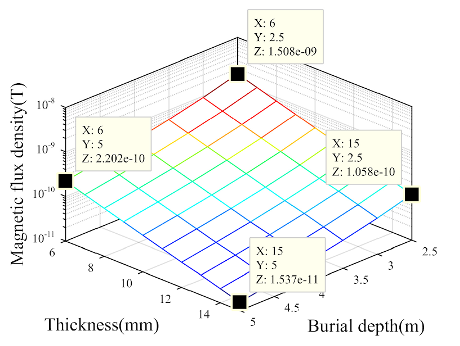
\includegraphics[scale=1]{Attenuation.png}
			\caption{ELF Attenuation Finite Element Analysis}
			\label{ELFAttenuation}
		\end{figure}

		\textbf{Solutions}
		
		\textbf{Filter}:
        One potential solution in order to overcome this challenge is the use of a simple filter and amplifier circuit.
        The sensors are wide-band antennas and many other frequency components are received together. This is a problem as low signal to noise ratio is a disadvantage for tracing and localization algorithm.
        Therefore, band-pass filter with high gain and high quality factor is one possible solution.
        \\
        \hspace*{3ex}\figref{filterDesign} highlights the function of a sensor circuit. 
        The output of the sensor is sent to filter and amplifier to detect the useful signal. 
        In this system, five-grade active filter is designed in order to get high gain and advanced quality.
        The filter consists of five segments including amplifier I (high pass filter), band pass filter I, amplifier II (band pass filter), band pass filter II and amplifier III (high pass filter).
        The output signal then consists of the emitted signal separated from the other frequency components. 
        
        \begin{figure}[h]
			\centering
			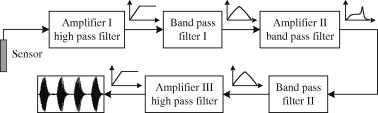
\includegraphics[scale=1.5]{Filtering.jpg}
			\caption{Filter Design} % This needs a citation for the source I think
			\label{filterDesign}
		\end{figure}
		
		Unfortunately, in order to attain a more ideal filter, a higher order filter must be used.
		This presents an issue as the impulse response is longer which pushes the latency higher and hence decreases accuracy in localisation. 
		Another issue is demonstrated in \figref{SNRPower}.
		The normalized power spectrum of three different signals, including noiseless ELF signals, narrow-band noise and ELF signals with noise are shown. 
		Since the frequency of narrow-band noise is concentrated at 23 Hz, it is difficult to discriminate between ELF signals and noise by frequency domain, which indicates that the frequency-domain information may not be useful for the detection. 
		Thus, the performance of the time-frequency analysis based filtering method is lower than a time-domain characteristic based FDT method.

         \begin{figure}[h]
			\centering
			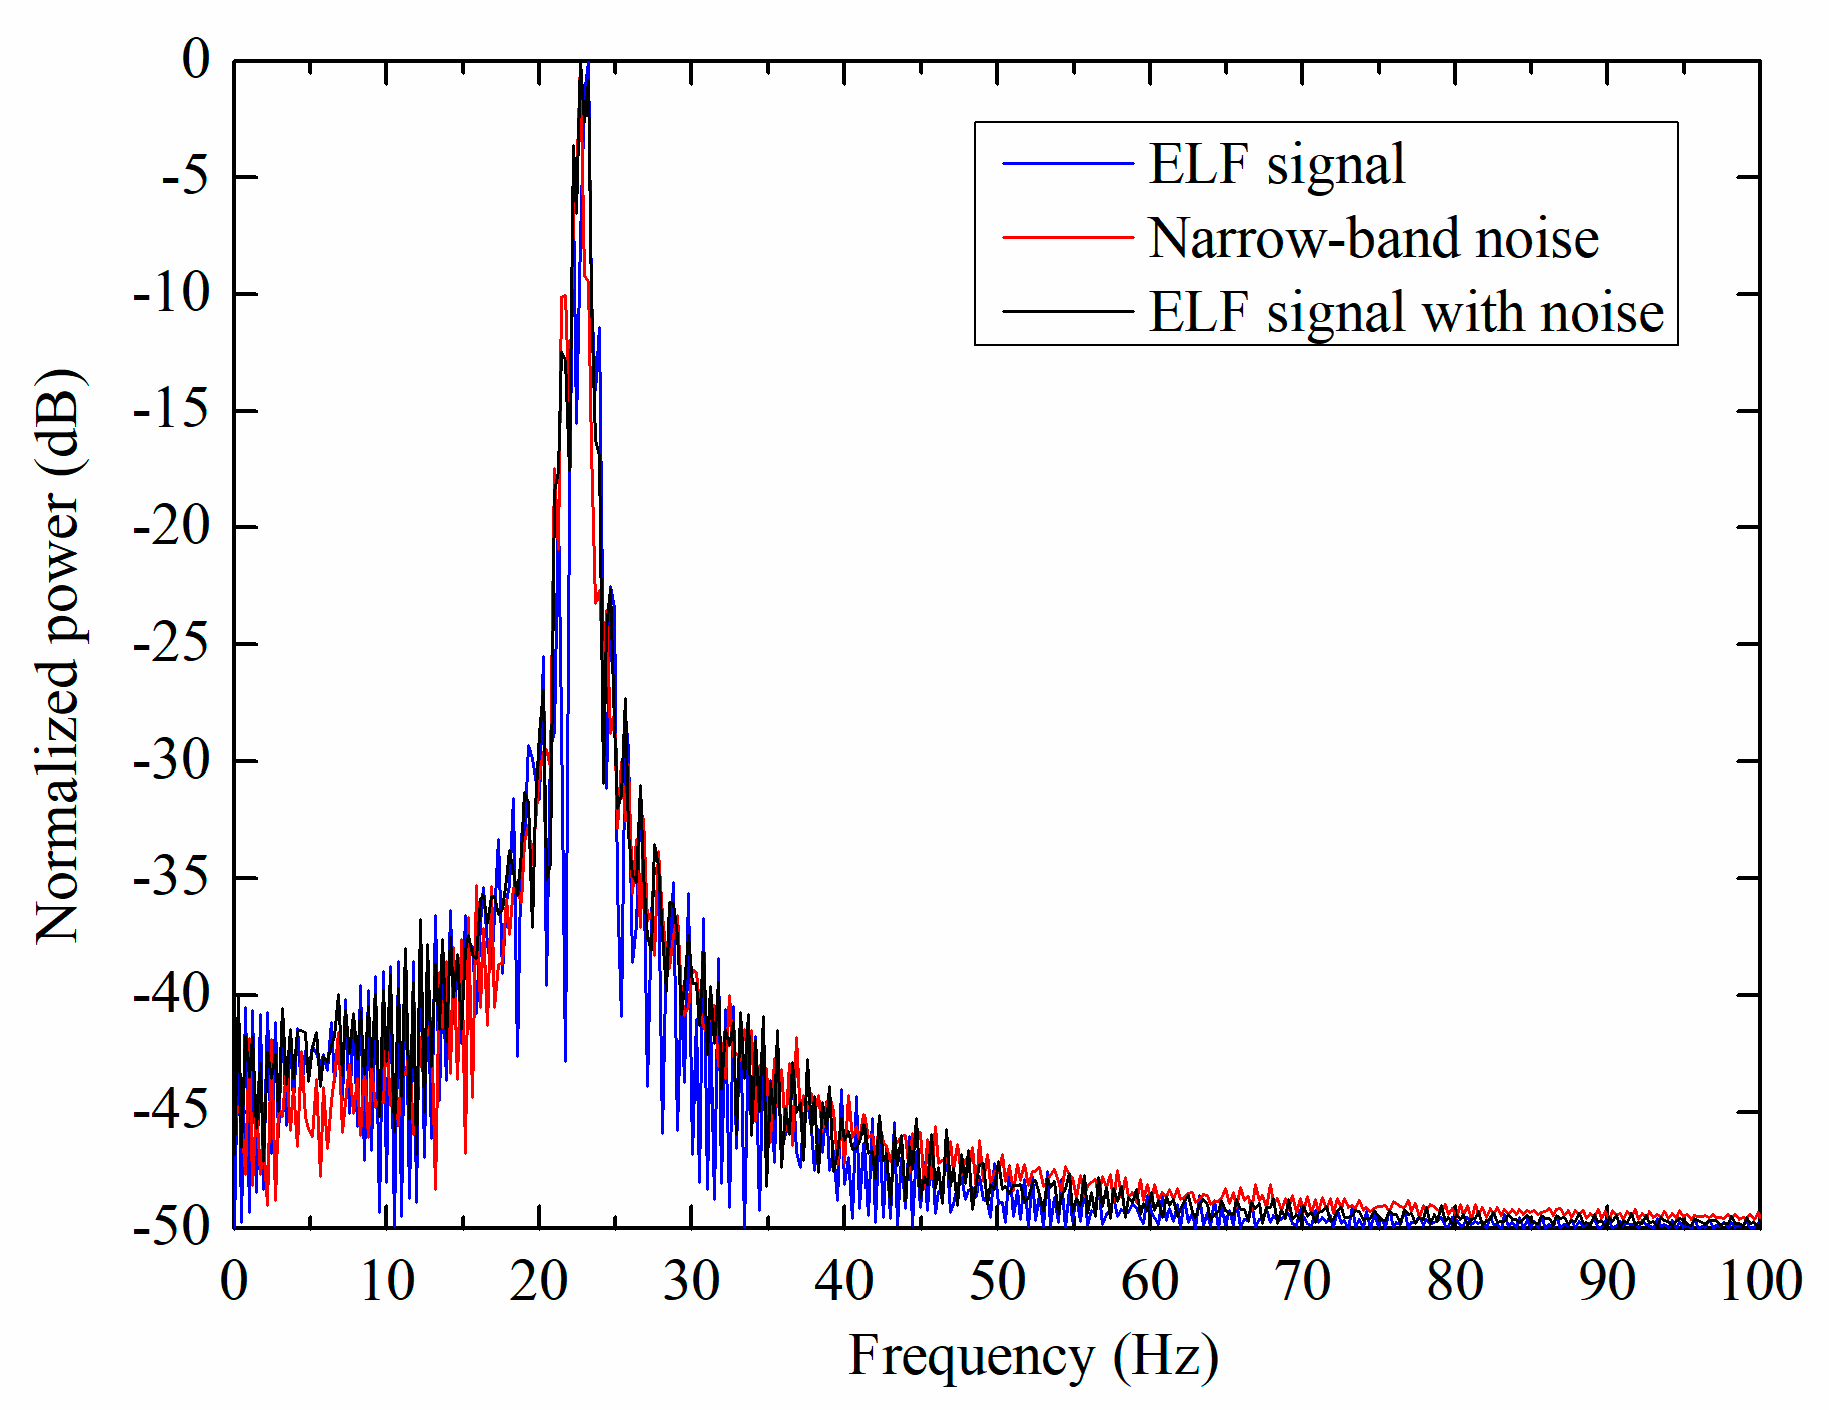
\includegraphics[height=\imageheight]{SNRPower.png}
			\caption{Normalized power spectrum when SNR is 0 dB and speed is 15 m/s.}
			\label{SNRPower}
		\end{figure}
	    
	    \textbf{Fast Decision Tree (FDT)}:
		Following the argument against the time-frequency based method outlined above, an improved solution is a time-domain method followed using a Fast Decision Tree. 
		\\
    	\hspace*{3ex}The overall architecture of the algorithm is shown in \figref{FDTFlowcahrt}. 
    	Firstly, a data fusion model was implemented in order to get a better signal representation by fusing the envelope decay rates through a least squares method. 
    	In this case, the envelope decay rates are the rate of the decay of the envelopes of the received X and Y axis ELF signals. 
    	Then, a Fast Decision Tree (FDT) algorithm is proposed to detect the ELF signals. 
    	The FDT first estimates the fused envelope decay rate to maximize the orthogonal signal power of ELF signals, and the maximized orthogonal signal power is used as the test statistic for the signal detection, which provides an excellent detection performance.
        
         \begin{figure}[h]
			\centering
			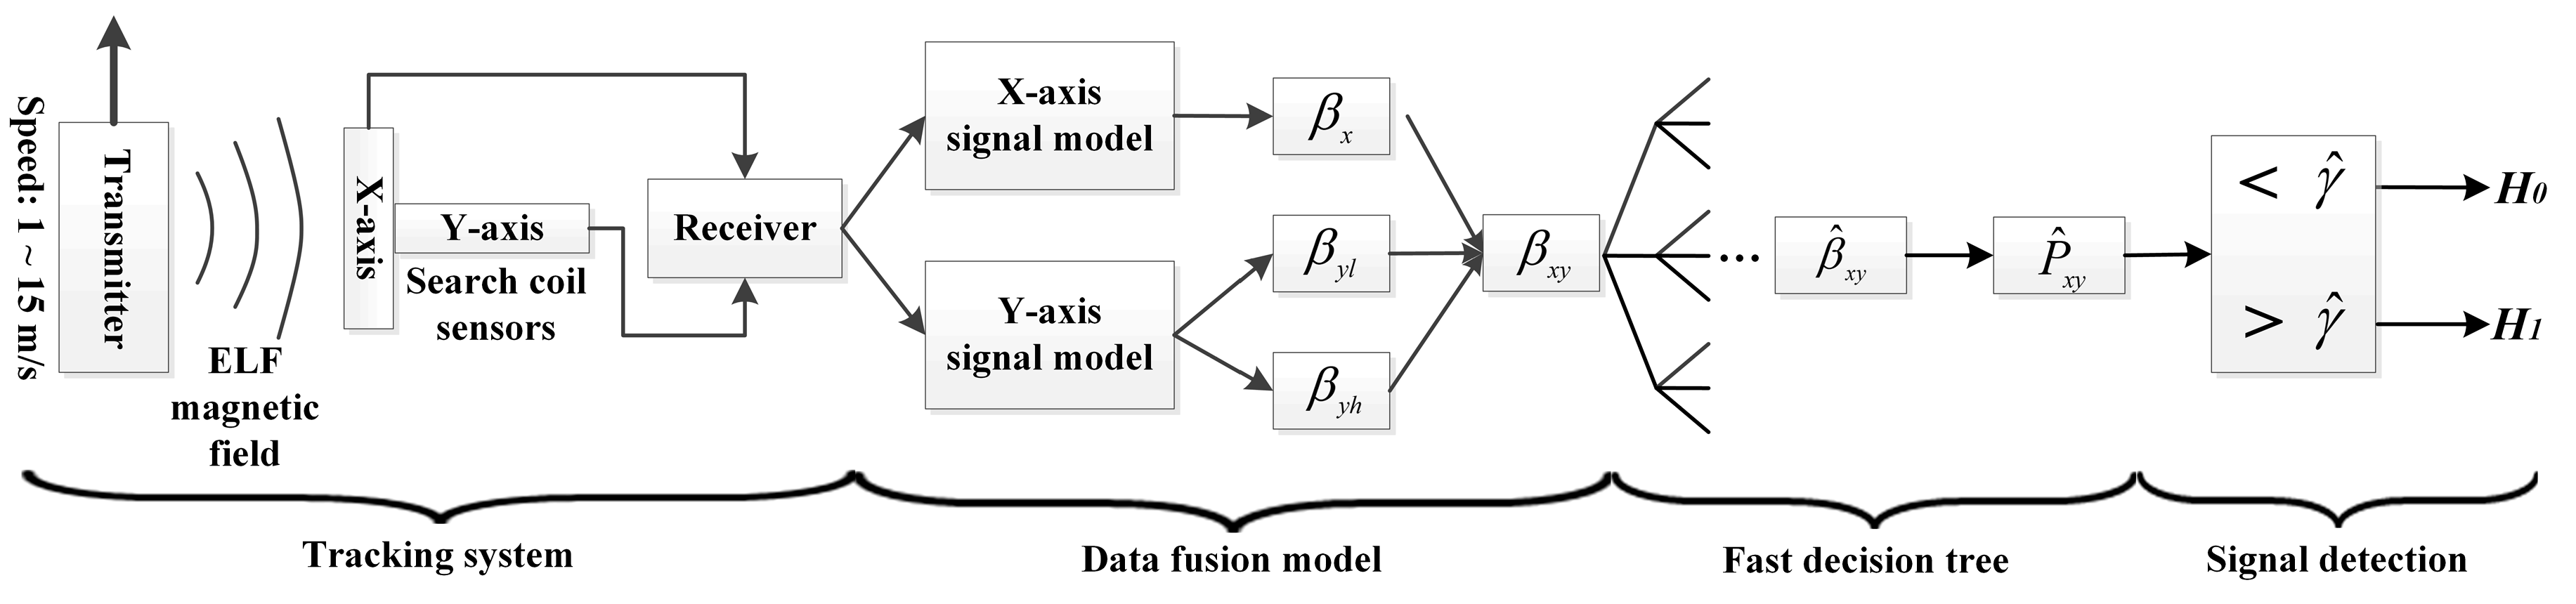
\includegraphics[scale=0.12]{FDT.png}
			\caption{Flow chart of FDT method } % This needs a citation for the source I think
			\label{FDTFlowcahrt}
		\end{figure}
		
		One of the main advantages of this approach is the low latency. 
		The fast calculation process of the FDT method removes the need for large matrix multiplication in the frequency domain. 
		This is particularly important as relaying the robots position as fast as possible ensures the GPS position it receives is as accurate as possible. 
		\\
    	\hspace*{3ex}Through following a time-domain method, the analysis of the normalized power spectrum suggests that it will improve detection performance over a time-frequency domain method. 
    	This is validated through field testing on a PIG containing an ELF transmitter of frequency 23Hz. 
    	Upon testing, the FDT method is close to the upper theoretical bound and the difference between them is less than 5\%  when SNR is 0 dB.
    	The experimental results further validate that the proposed FDT method can detect the short transient very weak ELF signals in real time. 
    	Based on these results, the proposed FDT method is validated to be effective in real-time pre-processing of the signal for localisation uses.
		
		\textbf{Localisation}\\
		Once the receiver has filtered the ELF signals, it must then use a localisation algorithm in order to obtain the global position of the robot. In our case, two methods of localisation will be considered. The criteria for assessment is practicality, accuracy and latency. 
		
		\textbf{Single Sensor Design}\\
		One simple design involves using a single filter and sensor module. This solution is commonly used for pig tracking in the above ground pipeline. As the robot passes the transmitter, the ELF waves induce a spike in the magnetic field detected by the receiver. This simple solution allows the location of the robot to be precisely determined when the position of the pipe is known relative to the receiver i.e directly below it. Along with excellent accuracy, the method also allows extremely low latency as little localisation processing is required. Further, given that only one sensor is required, the receiver is simple and cheap to design. \\
    	\hspace*{3ex}However, in the case of our robot, inspecting underground piping means that the pipe position is not always known relative to the robot's position. Further, if we were to discern the position of underground piping from maps, no further accuracy would be added by using an external localisation system over using the internal localisation system. 

        \textbf{Multiple Sensor Design}
		
		Given the problem the previous solution faces a challenge with localising the robot without accurate knowledge of the pipes positioning, an improved solution will use multiple sensors in order to localise the robot. With this solution, no prior knowledge of the pipe location is needed as the receiver is capable of calculating the relative distance of the robot from itself. Then, the algorithm will again use the GPS capabilities of the receiver in order to calculate the robot's global positioning. \\
		
		\hspace*{3ex}The algorithm presented works by solving an inverse problem. Each sensor receives a different intensity of magnetic field strength, and each presents an equation. Given there are five unknown parameters to be solved, the initial position in 3D space and the orientation to each axis, at least five sensors are needed. However, if cost and complexity are not considered, a higher number of sensors provides greater accuracy and eliminates greater noise disturbances. In this case, the localisation algorithm is overdetermined and a nonlinear method such as least squares can be applied. Figure x provides a demonstration of the robot's positioning and the receiver.\\
		
		\begin{figure}[h]
			\centering
			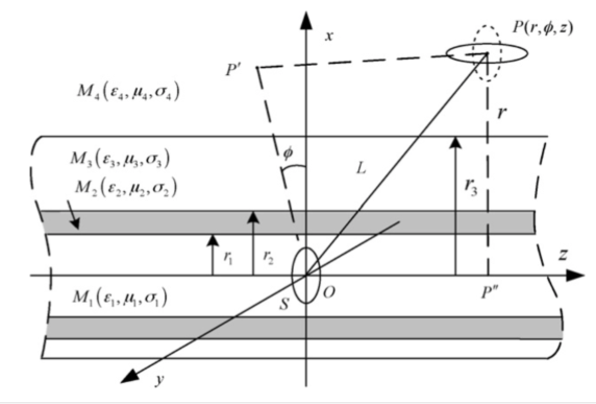
\includegraphics[scale=1]{localisation.pdf}
			\caption{Geometry of Buried Pipeline}
			\label{localisation}
		\end{figure}
		
		The outlined algorithm presents a simple solution to localisation that improves upon the single sensor design. However, the model does make some simplifying assumptions. Firstly, the attenuation effects in the material above the pipeline is ignored. This assumption is reasonable given the low conductivity of soil and air compares to the pipe. Additionally, the sensor also relies on the fact that the pipeline is of constant thickness. This creates accuracy problems if the pipeline is of different thicknesses. Therefore, one possible extension of this algorithm is to consider a way to account for this variation. 
		
		
		
		
		
	\section{Estimated Cost \& Weight - ENG}
		
		In order to estimate the cost of the robot it was necessary to select some sample components which are discussed below.
		These components also provided a reference point for the weight of the robot, allowing us to consider the requirements for forces and evaluate the likelihood of the robot causing damage to the piping system.
		
		% Also get estimated weight from selected components?
		\subsection[Locomotion]{Locomotion - Jim Laney}
		
		In order to determine suitable components, the main parts of the locomotion system which require acquisition must be considered.
		The parts which will be considered here are the track modules, the linear actuators, the internal rotation motors and the legs and gears.
		\\
		For the track module, the best reference point was the Inuktun Minitrac, a larger version of the Inuktun Microtrac module used by Ciszewski et al.\supercite{ciszewski2015design} for their testing of a pipe inspection robot.
		These cost $£ \ xxx$ each, and three are required for each leg of the robot, bringing the overall cost to $£ \ 9xxx$.
		They are probably over specified, as each has a pull rating of roughly $30$ kg for continuous duty, meaning the robot can weight up to $270$ kg, which would be an unrealistic and impractical figure to aim for\supercite{inuktunTracks}.
		Each module can be provided in either aluminium, brass or steel, with the main difference being the weight.
		Aluminium was chosen, as it is the lightest of the three, but each module still weighs $5.7$ kg taking the track weight to $51.3$ kg for all 9 track modules.
		As this is quite heavy, a different design could be considered, with a motor driving the tracks instead, so a new system can be designed to minimise the weight.
		Additionally, while discussing the pricing and operation with a representative from Eddyfi Technologies, it was made clear that the Minitrac is no longer for sale for commercial uses, as they found that they were often being used in products which compete with Eddyfi's own pipe inspection robots.
		However, these track modules give a reasonable indication of the eventual cost to expect for the robot.
		\\
		The sample linear actuators chosen were selected as they have $200$N of force output and a potentiometer to measure the extension of the actuator\supercite{rsproLinear}.
		Using \equationref{maxWeight}, reproduced below, values for the worst case scenario can be estimated.
		\begin{align*}
			W &= \frac{6 \mu_{t,p} F \tan \left( \theta \right)}{\cos \left( \phi \right)}
		\end{align*}
		The worst case scenario occurs when when $ \mu = 1.21$\supercite{sato2011development}, $\theta = 10^\circ$ and $\phi = 0^\circ$, as stated before.
		This gives us a maximum weight of $528.5 N = 53.9$ kg, which is quite large, although comparatively small compared to the estimated weight of 9 Inuktun MiniTrac modules, hence why they would be considered inappropriate.
		With a safety margin of 1.5 for the linear actuator output, limiting their output to $130 N$, the maximum weight becomes $343.5 N = 35.0$ kg which is still reasonable and significantly larger than similar robots.
		These cost $£ \ 121.46 - £ \ 132.02$ each depending on quantity, but the lower price can be used as this is for 10 or more actuators, which is less than 2 robots. 
		Thus the actuator cost for a single robot would be $£ \ 728.76$ since 2 linear actuators are used for each leg, meaning a total of 6.
		The overall weight of these linear actuators would be $0.504$ kg, which is negligible compared to the weight of most of the other components, as well as the estimated weight of the robot shell.
		\\
		The next part to consider is the motor used for rotation of the legs relative to the body. There is no specifications required for this at the moment, but a high torque motor would be ideal.
		A sample product which is both relatively small and high torque was selected\supercite{rsproRotation} as it has a maximum output torque (at stall) of $1.46$ Nm.
		The diameter of the actual motor is only $42.8$ mm, meaning that there is plenty of space to use a larger more powerful motor if testing reveals that it will be necessary.
		The cost of these drives is $£ \ 141.84$ per motor, and 2 are required for the main body of the robot.
		Since similar motors could be used as the RC servo motors in the active compliance joint, another 3 would be included in the robot, bringing the total cost for 5 rotation motors to $£ \ 709.20$.
		\\
		\begin{figure}[h]
			\centering
			\begin{multicols}{3}
				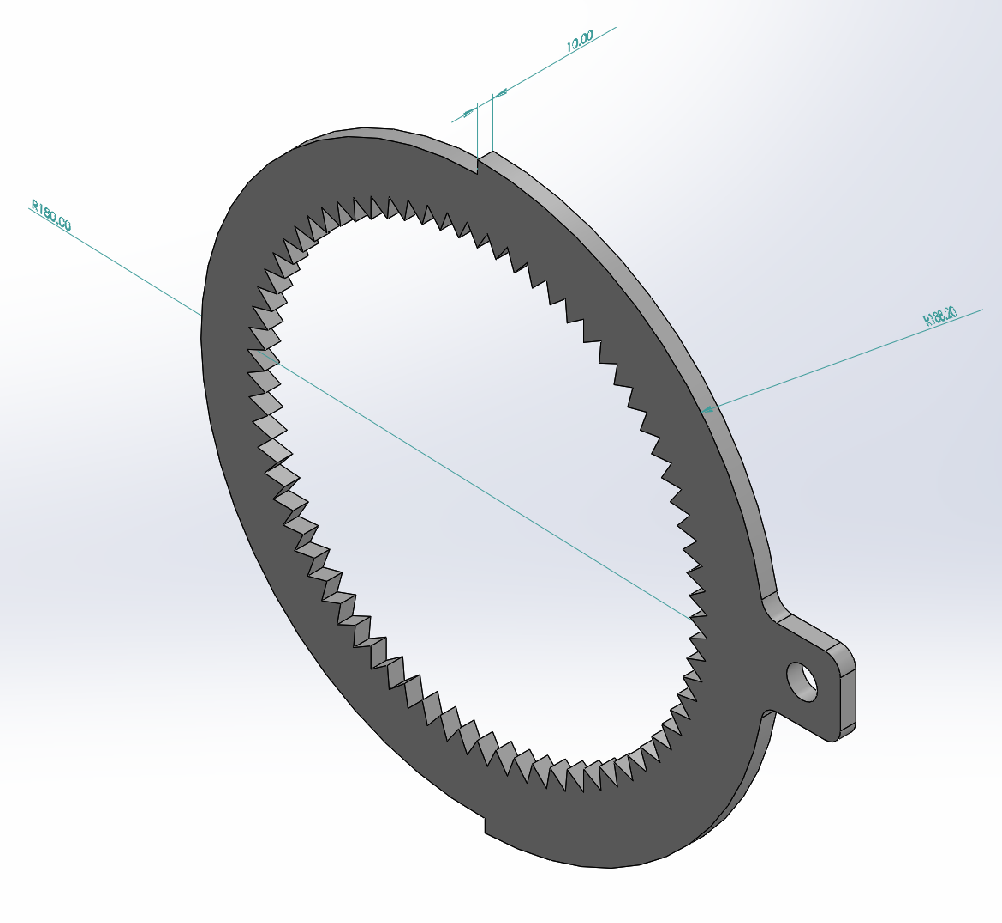
\includegraphics[height=0.23\textwidth]{gearCAD}
				\caption{Aluminium gear used as the outside of the planetary gear, with dimensions}
				\label{gearCAD}
				\columnbreak
				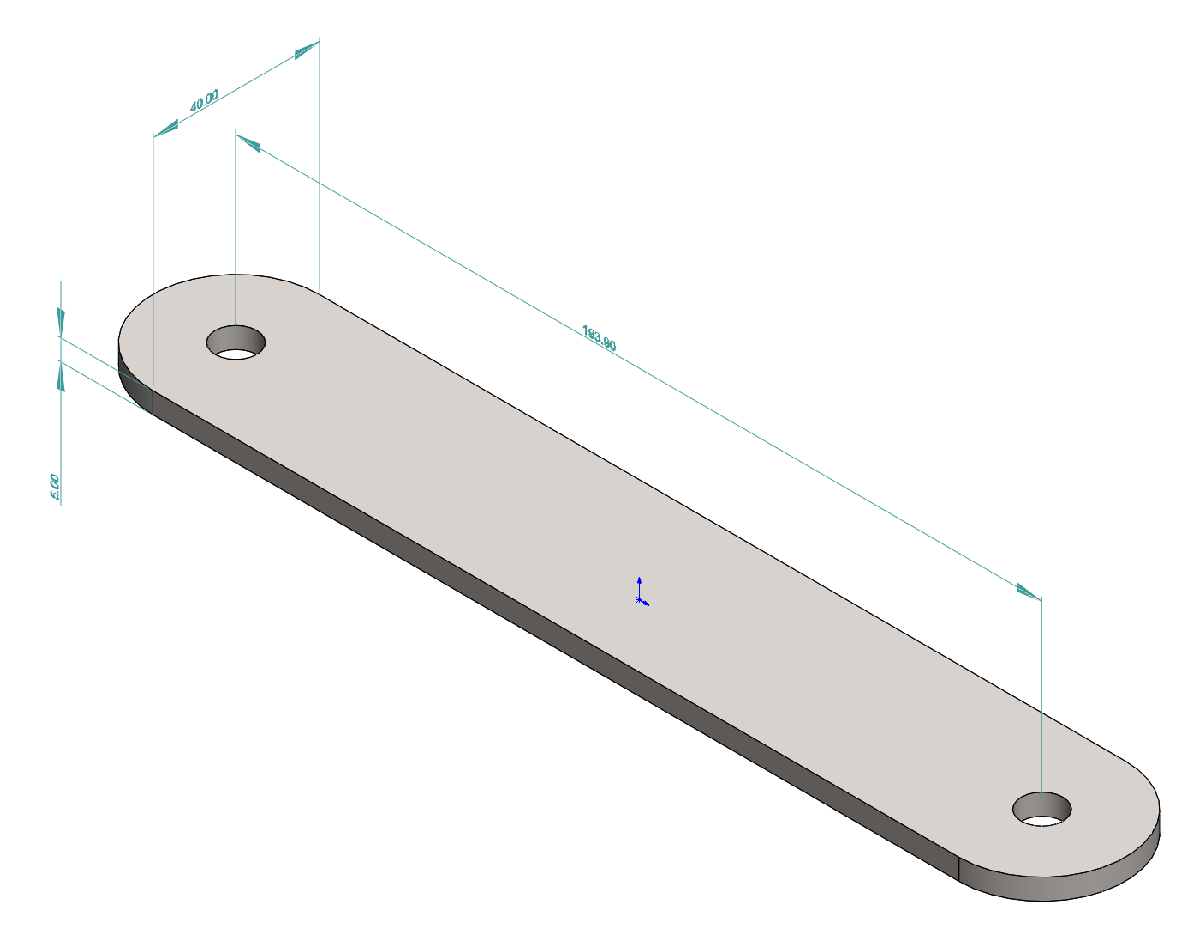
\includegraphics[height=0.23\textwidth]{shortLinkCAD}
				\caption{Stainless steel short link of the leg mechanism with dimensions}
				\label{shortLinkCAD}
				\columnbreak
				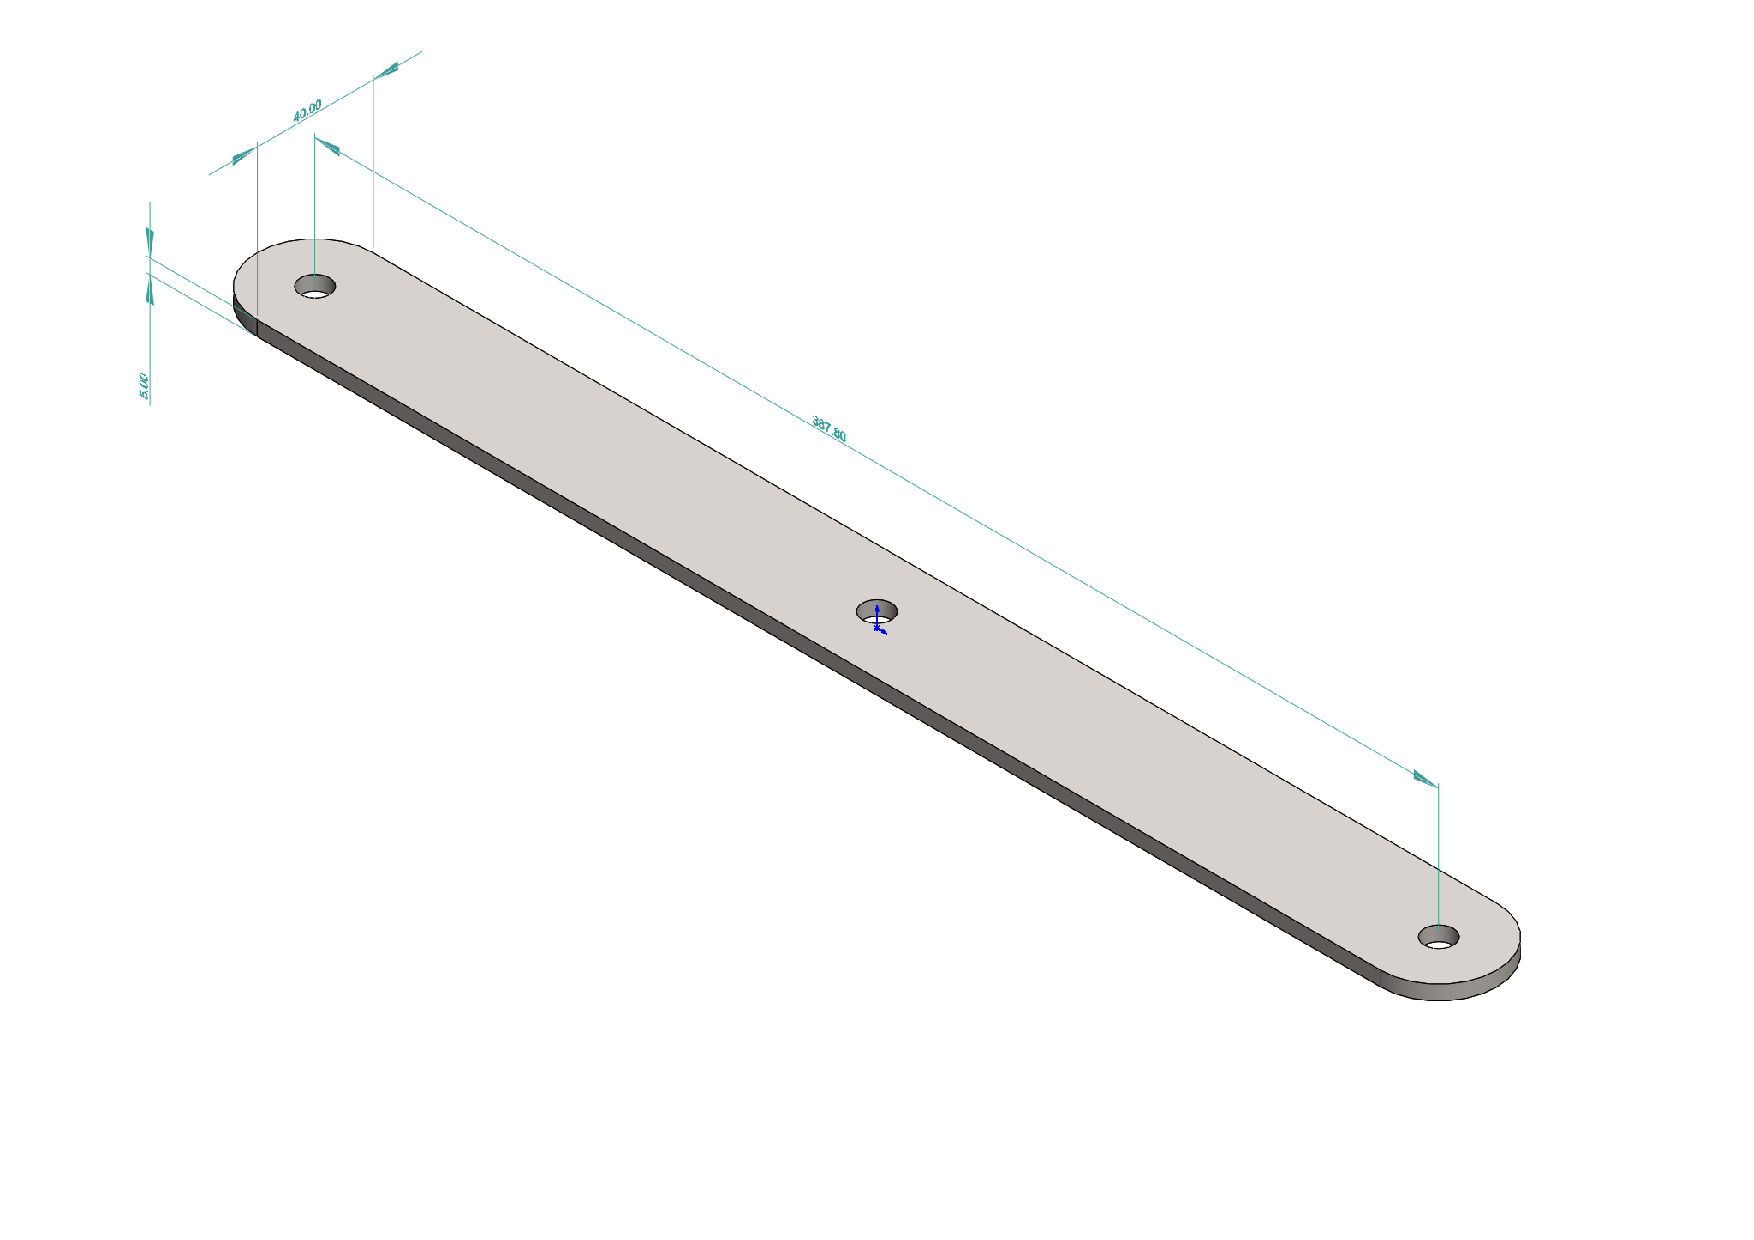
\includegraphics[height=0.23\textwidth]{longLinkCAD}
				\caption{Stainless steel long link of the leg mechanism with dimensions}
				\label{longLinkCAD}
			\end{multicols}
		\end{figure}
		The remaining components of the locomotion system were estimated using the 3D CAD models, shown in \hyperref[gearCAD]{Figures \ref*{gearCAD}, \ref*{shortLinkCAD} \& \ref*{longLinkCAD}} to estimate their volume.
		The leg pieces were assumed to be made out of stainless steel, and the gear was to be made of aluminium.
		The density of stainless steel is $7900$ kg m\textsuperscript{-3}\supercite{HLT}, so the longer link weighs $0.653$ kg and the shorter link weighs $0.350$ kg.
		Thus, a single leg, which is made up of 2 short links and 2 longer links, weighs $2.00$ kg, bringing the total contribution of the three legs to $6.02$ kg for the whole robot.
		The density of aluminium was assumed to be $2700$ kg m\textsuperscript{-3}\supercite{HLT}, which makes the weight of a single gear $3.42$ kg, and there are 4 inside the robot, bring the total weight up to $13.68$ kg
		This could be mitigated by refining the design, as this is a very rough sketch of the gear, and is probably thicker than would be necessary in reality.
		
		\subsection{Power}
		
		\subsection{Sensing}

		\subsection{Communications}
		Having outlined the communication hardware earlier, it is now necessary to determine the cost and weight for each component. Again, where an existing component’s cost or weight is not available online, an estimate will be made using similar products as references. 
		
		\textbf{Cable}\\
		From the hardware analysis of the cable, it is justified that the tensile stress the cable will experience is far less than the maximum tensile stress of even a thin 5mm kevlar pure cable. In the interest of weight, it is desired that the cable therefore be as thin as possible whilst maintaining a safety factor of at least a factor of 10 in tension. Further, given the minimum bend radius for optical fibre is often suggested as being 20X that of the diameter, a smaller radius will ensure this criteria is met.\\
    	\hspace*{3ex}Fibre optic company MacArtney offers a solution which meets these requirements. The cable consist of 4 inner single core fibre optic cables which are then reinforced with kevlar braiding. The overall cable is 9.1mm thick, weighs 91kg/km and offers a tensile strengths of 2.5kn. The cable also requires a minimum bend radius of 110mm which is suitable for our robot. \\
    	\hspace*{3ex}In terms of price, the wire costs £ xxx and a total of 1000m are required for the operation of our robot. This brings the overall weight to 91Kg at a cost of £ xxx 

        \textbf{ELF Transmitter}\\
        For the ELF transmitter it is more difficult to estimate the weight due to the complex range of components required. In order to make an estimate, the ELF transmitters supplied by PolyEurope are taken as reference. The PTI - 29980 is a solution offered for pipes greater than 200mm in diameter and has dimensions of 298mm in length and 98mm in body diameter. Although this includes the outer stainless steel casing which would not be required as we would house the transmitter inside the robot, an upper limit on weight is provided as being 6.8kg.\\
        \hspace*{3ex}Again, with difficulty estimating the cost of individual components, the price of PolyEurope’s solution is taken as a comparison. This solution provides an upper estimate to the cost of the transmitter as £ xxx. 
    
        \textbf{Other Costs}\\

        
        Since the cable reel and ELF receivers are not carried by the robot, their weight is not a consideration here. However, the price of these hardware components is important in order to assess the total cost of the robot. \\
	    \hspace*{3ex}As outlined in the previous section, the price of the identified cable reel that is going to be used is £ xxx. The price of the receivers is more complicated to calculatem. The total cost of the receivers is dependent on the accumulated errors of the internal localisation system. Given the internal errors become significant over a distance greater than xm, it is required to have a receiver every xm in order to correct this error. Again, through using the company ProPipe as a reference for their above ground receivers, an estimated cost per receiver of £ xxx can be made. Therefore, over a distance of 1000m, the total cost would be £ xxx. 




		\subsection{External Hardware}
		% Does not need to be included in the weight calc obviously
		
		\subsection{Total Cost and Weight of Robot}
			
	\section{Industry Analysis - EEM}
		
		It was decided to use the Porter's Five Forces model\supercite{porter2008five} to analyse the in-pipe inspection robot industry, in order to provide a systematic analysis of the existing and possible threats to the company in the future.
		
		\subsection[Threat of New Entry]{Threat of New Entry}
				
		\subsection[Power of Suppliers]{Power of Suppliers - Jim Laney}
			
			The power of suppliers in the in-pipe robotics industry is typically very minimal, due to the large number of substitutes for a given product.
			As an example,the components selected for the robot will be used to evaluate the overall power which suppliers hold in the industry.
			\\
			The non electrical components, such as the robot body, robot legs and leg gears are all made of either aluminium or steel, which are readily available from many sources, meaning it is very difficult for a single supplier to exert any influence over the user.
			Similarly, all of the generic electrical components, such as the motors used for rotating the legs and eventually the wheels, the linear actuators and different sensors used for measuring the position of the robot are easily replaced, as there are many suppliers of similar products.
			There are some specific products, such as the industrial cameras, AHRS and the laser scanner, which have far fewer substitutes, due to their more specialised nature, but these still can be replaced with competitive products relatively easily without making major changes to the robot.
			\\
			The other electronics, such as the graphical processing unit (GPU) and  also have alternatives to a greater or lesser degree.
			There are not many major GPU manufacturers, with AMD, Nvidia and Intel dominating the commercial market\supercite{rake2020graphic} due to long term presence in the market.
			Thus these manufacturers have greater power over companies which have on board image processing, and can dictate the cost and functionality of  products.
			As such, these suppliers offer the greatest threat to the in-pipe robotics industry.
			\\
			Within the fibre optic industry in the UK there are only 3 major companies\supercite{neve2020fibreoptic}, which have a total market share of $22.8$\%, but of these only Leviton and Prysmian are possible suppliers.
			The rest of the industry is made up of much smaller firms who supply niche products for optical fibres, so there are a maximum of 3 or 4 suppliers.
			This means that these companies will also exert significant pressure on the in pipe robotics industry, but still do not have the level of influence that the GPU manufacturers do.
			\\
			Finally, the threat of forward vertical integration is practically non-existent, due to the large variety of suppliers.
			While there are a few key suppliers who exert significant influence over the industry, none of these are in a position to easily move into the in-pipe inspection industry as they would be required to have many of the same suppliers that current companies do.
					
		\subsection[Power of Buyers]{Power of Buyers}
		
		\subsection[Threat of Substitutes]{Threat of Substitutes - Jim Laney}
			
			The threat of substitutes in the in-pipe inspection robot industry is medium, as there are many established substitutes which currently dominate pipe inspection services.
			\\
			The main threat is the manual inspection of pipelines as these can inspect all kinds of pipes, just like robotic solutions and have a much lower up front cost.
			As well as this, manual inspection has the advantage of familiarity as it is an established practice which gas pipe companies know they can rely on.
			Manual inspection uses different methods for inspecting pipes dependent on the the kind of damage being inspected for.
			\\
			For external corrosion inspection, a pre-assessment is performed, followed by both indirect and direct inspection techniques being used, the latter of which requires excavation to occur for that section of the pipe\supercite{kishawy2010review}. 
			For internal corrosion inspection, a similar process is followed, with pipes that have the greatest inclination being inspected first to identify the location of localised corrosion. 
			However, both these methods require excavation in order to confirm the location of the corrosion, which is disruptive, especially in urban environments.
			\\
			When checking for cracks manual inspection can typically only find these when a leak has occurred, as there is otherwise very little change in behaviour of the gas inside the pipe.
			Thus, manual methods rely on constant assessment of conditions within the pipe, such as the mass-balance method, pressure-drop method and using gas smelling dogs\supercite{kishawy2010review}.
			Ground penetrating radar is also used as another method for looking for cracks without excavation, but visual inspection is also typically used to ensure accuracy of the readings, which does require excavation.
			Computer models can also be used to predict the behaviour of the pipeline in order to predict faults, but as this requires modelling of complex fluid dynamics, these are not always reliable.
			\\
			Pipeline Inspection Gauges (PIGs) are the other main substitute to robotic in-pipe inspection, as these are passive devices which are forced along the pipeline by the gas flow.
			However, PIGs are uncontrollable and cannot operate in pipelines containing sharp bends\supercite{mills2017advances}, making them unsuitable for urban pipelines.
			As such the threat from PIGs is minimal since the robot has been specifically chosen to enter an area where they are not currently suitable, although it is possible that more advanced PIGs may be developed in the future which could compete in urban pipelines.
			\\
			Another significant substitute is the use of pipeline models to predict damage in order to decide when to replace pipes, rather than using inspection techniques.
			This reduces the requirement for inspection solutions in general, as models can be used to predict when pipes will fail meaning inspection is no longer required.
			However, inspection is still needed in order to provide initial data for the model, and models are still not particularly accurate at predicting failure timings\supercite{zakikhani2020review}.
			In particular, models typically consider limited causes of failure, most often corrosion or third party damage, and only consider a single failure mode for the pipe, or instead not differentiating between failure modes.
			As well as this, current failure prediction models are not generalised, and require either extensive historical data which will not always be available or are designed to predict the failure of a single case study pipeline.
			As well as this, all pipeline failure models are conservative estimates, meaning they suggest damage will occur before it is feasible, and as such lead to loss of profit, and also lead to pipes having to be disconnected for repairs which may not be necessary.
			Thus the threat of substitution entirely by models of pipe failure is low, but the likelihood of in pipe robots working alongside failure models to help verify and improve them is higher, slightly reducing the market size for inspections.
		
		\subsection[Rivalry Among Existing Competitors]{Rivalry Among Existing Competitors - Louis Emanuel}
			High intensity of competitive rivalry can make an industry more competitive and thus decrease profit potential for the existing firms\supercite{porter2008five}. This section will serve to analyse the level of competitive rivalry that our robot would face in the in-pipe inspection robot industry. \\
	        \hspace*{3ex}There are a number of different factors that determine the level of competitive rivalry such as concentration in industry, switching costs, differentiation, and exit barriers\supercite{rivalryfactorsCI}. And hence this section is structured to consider each of them in turn. 
	        
	        \textbf{Concentration in industry}\\
	        If an industry has a high number of competing firms with similar offerings, the level of competitive rivalry will be high. In comparison, a monopoly market structure is dominated by a low number of firms and will exhibit less rivalry. Consequently, the level of market concentration significantly impacts the competitive rivalry.\\
	        \hspace*{3ex}In our case, there are a low number of firms currently operating in the autonomous in-pipe inspection market. With the only significant competitor being ULC Robotic’s CISBOT\supercite{cisbotbeast}. However, if we consider the whole pipe inspection market, there are a significant number of similar sized competitors that use PIG technology including SGS, Pigtek LTD and Propipe among others. PIG technology does not have automated capabilities, and so its product offering is significantly different than the one we are proposing. Therefore, given the only competitor with similar offerings is Cadent, the market exhibits a monopoly structure and suggest a low intensity of rivalry.
	        
	        \textbf{Switching Costs}\\
	        Aside from fixed costs, switching costs also influence the extent of rivalry as high switching costs in an industry will lead to a decrease in competitive rivalry. These switching costs arise from the fact that customers who have invested a lot of resources in learning to use a product will find it costly to switch to a competitor. \\
	        \hspace*{3ex}The impact of switching costs on competitive rivalry depends entirely on the business model of our robot. For example, an outsourcing approach in which the customer hires the robot and an operating team will have far lower switching costs than purchasing the robot outright and training an internal team to operate it. Looking at current competitors, ULC’s CISBOT is not sold outright, but operates using service contracts. Therefore, the switching costs are currently low in the industry which suggests a higher intensity of rivalry. Although, this may be favourable for a new entrant. 
	
	        \textbf{Differentiation}\\
	        The degree of differentiation also determines how intense the competition will be. If a firm in the market is offering highly differentiated products that other organizations cannot easily imitate or copy, then it will face relatively less competition.\\
	        \hspace*{3ex}Again, considering the overall in-pipe inspection market, since PIG’s are incapable of currently operating in the urban pipeline environment our robot will be inspecting, we have a distinct differentiated capability. However, Cadent is capable of operating in this environment and also offers a pipe fixing capability. Whilst our robot does not offer this, it does offer automated capabilities and at a significantly lower price. Therefore, given our different offering to current firms in the industry, we would expect a lower threat of rivalry. 
	        
	        \textbf{Fixed Costs}\\
	        The specific costs a firm faces to operate in a market can also affect how intense the threat of rivalry is. Costs that can increase rivalry include high fixed costs and high storage expenses. To cover these, competitors in a market will need to operate at high capacity and this is likely to intensify competition.\\
	        \hspace*{3ex}Considering the in-pipe inspection market, the small size of robots and PIG’s means that only a small amount of storage space is needed. Also, the small production volumes suggest that the manufacturing resources required are low. However, one significant fixed cost for the industry may be interest payments associated with creating the robots. Given the complex technology, robots like CISBOT are priced at \$1 million. This could be problematic as given the service contract business model it operates, this investment will likely not be recuperated for a significant period of operation. Despite this, the robot we offer is far cheaper and so the contribution of costs to the threat of rivalry are low. 
	        
	        \textbf{Conclusion}\\
	        Overall, from an analysis of the key factors that Porter outlined as contributing to a high level of rivalry, the threat level is determined as low. The only exception being the low switching costs currently in the industry. However, for our robot attempting to penetrate the market, this factor may be favourable due to the current monopoly CISBOT has. Given this low threat of rivalry, we can conclude that the industry has a high profit potential.

	\section{Customer Industry Analysis}
		% Insert Monty's P5F here
		Since there is only one customer industry, it is important to analyse the safety and sustainability of that industry to ensure that the business was secure.
		The Porter's Five Forces model\supercite{porter2008five} was once again used to analyse the gas pipeline inspection industry.
			
		\subsection[Threat of New Entry]{Threat of New Entry}
				New entrants are motivated to enter the gas distribution industry due to the high profits achieved by current firms which leads to increased competition as they strive to gain market share. The extent of this threat depends on the current barriers to entry in the industry. Porter outlined key barriers as being economies of scale, technical knowledge and regulation. And hence the following section will analyse each of these factors. \\
				
				One barrier to entry in the Gas distribution industry is economies of scale. The main distribution networks each cover a significantly sized region of the UK. Therefore, through being able to bulk purchase pipeline, hire permanent specialist employees and achieve cheaper financing, established companies such as Cadent who operates 82,000 miles of gas pipes have a significant advantage which deters new entrants. \\
					\begin{figure}[h]
			    \centering
		    	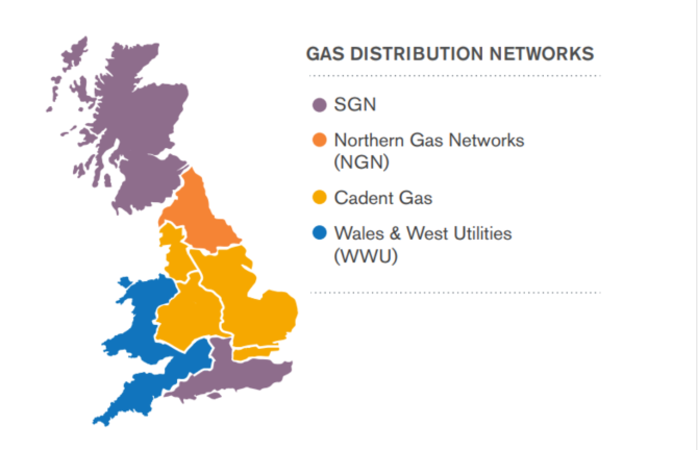
\includegraphics[scale=0.8]{distribution.pdf}
			    \caption{UK Gas Distribution Networks} % This needs a citation for the source I think
		    	\label{distrit}
	        	\end{figure}
				
				Another significant advantage our customers have is technical knowledge. SGN for example has over 85 years of experience working in the gas distribution industry. Therefore, in order to compete, new firms must acquire personnel with knowledge of the complex processes involved in construction, maintenance and replacement of gas pipes. \\
				One of the most significant barriers to entry is the regulation and relationships current companies have with regulators and suppliers. Looking at the big four gas networks, each is heavily regulated by Ofgem. Further, in order to distribute gas, a license must be obtained which limits the amount of revenue gas distribution companies can recover from customers. This thereby makes the profit margins even smaller for new entrants. \\
	            \hspace*{3ex}Another key factor is the relationship gas distributors have with suppliers. Ultimately, without relationships with gas suppliers such as British Power, the gas distribution companies are incapable of supplying gas to customers. And consequently the success of our customers is heavily reliant on maintaining strong relationships gas suppliers.

			    \textbf{Conclusion}\\
                In conclusion, the threat of new entrants in the gas distribution industry is determined to be low as currently the barriers to entry are very high. In fact, the regulator Ofgem states on their website that they serve to regulate the gas distribution industry because ‘Gas Distribution Networks are natural monopolies’. These natural monopolies have an overwhelming advantage over potential competitors

		\subsection[Power of Suppliers]{Power of Suppliers}
		
		\subsection[Power of Buyers]{Power of Buyers}
		
		\subsection[Threat of Substitutes]{Threat of Substitutes}

		\subsection[Rivalry Among Existing Competitors]{Rivalry Among Existing Competitors}
		
	\section{Stakeholder Analysis - EEM}
	
		The main stakeholders for the project are individually analysed below.
		There were 3 major stakeholders identified - gas distributors, regulatory bodies and traditional inspection \& maintenance companies - and 3 minor stakeholders identified - gas suppliers, local councils and the general public.
		
		\subsection[Gas Distributors]{Gas Distributors}
		
		\subsection[Regulatory Bodies]{Regulatory Bodies - Jim Laney}
			
			The main regulatory bodies to consider are the Office of Gas and Electricity Markets (OFGEM), the Energy Networks Association (ENA) and the Health and Safety Executive (HSE).
			As well as this, regulations enforced by the Institution of Gas Engineers and Managers (IGEM) and the International Standards Organisation (ISO) are also of interest.
 			\\
			OFGEM is the UK government body which provides codes and regulations for the gas pipeline companies to follow, but these are mainly focused on reducing competition between gas transporters and ensuring a fair playing field for all companies.
			The Uniform Network Code (UNC)\supercite{joint2005uniform} covers the transition from a single national system to the current 4 provider network, as well as the rights of customers and independent gas transporters.
			The UNC also ensure that there is a fair market and safe operation for the gas pipe system, as well as encouraging the implementation of robust computer systems and daily energy balancing.
			While the safety sections of the UNC could be relevant to the robot, they are far too general, and are simply an overview of the responsibilities of the gas providers to ensure safe pipelines.
			The Independent Gas Transporter Uniform Network Code (iGT UNC)\supercite{igt2021independent} defines more about the interrelations between different smaller, independent providers and helps to standardise the interactions with gas providers.
			It refers to the UNC in large part, but focuses more on the responsibilities of Independent Transporters who are not the customers for the robot, and as such do not need to be focused on.
			The Supply Point Administration Agreement (SPAA)\supercite{spaa2021supply} is about supplier-supplier relationships which may not be covered by existing contracts, and contributes to the smooth running of the industry, and allows for smooth transfer of customers between different gas carriers.
			Finally, the Smart Energy Code (SEC)\supercite{smart2021smart} defines the rights and obligations of energy suppliers, transmission companies and other companies involved in metering in Great Britain.
			Since inspection of the pipeline is the main focus of the robot, the rights given by the SEC are not a concern.
			\\
			OFGEM also awards money to companies which they believe are innovating in new technologies as part of the National Innovation Competition (NIC).
			The NIC provides up to £20 million funding for innovation in the gas energy networks, although in 2020 £27.17 million was awarded under plans to move to increase overall funding to £28 million\supercite{ofgem2020nic}.
			However it also significantly easier to get the gas funding than electricity funding as the competition is significantly smaller - in 2020 there were only 2 applications, both of which were funded.
			Thus providing a compelling reason for the robot to receive NIC funding will be incredibly important in order to secure funding for development.
			\\
			The ENA is the industry body for all the energy suppliers in the UK \& Ireland, allowing them to publish all their own guidance as to what is required to operate safely within pipes.
			For the gas industry, these fall under the Gas Industry Standards (GIS), which define both how the robot can operate within pipes as well as how the pipes should be built and maintained.
			However, most of these standards refer to traditional methods of pipe inspection and as such are not directly applicable to the robot.
			The most likely to affect the robot design is GIS/F10:2015 “Ancillary fittings used for the live insertion of gas mains operating at pressures equal to or less than 75 mbar”\supercite{energy2015gas}.
			GIS/F10:2015 describes how the insertion of polyethylene pipes into steel gas mains must be performed on low pressure lines, which may provide guidance on the insertion of the robot into similar pipes.
			However the pipes specified by 	GIS/F10:2015 are 8 inches (203.2 mm) in diameter, which is much smaller than the pipes the robot is designed to operate in and operating pressures are higher, so this standard will be of limited use.
			\\
			The HSE is the government agency responsible for the regulation of workplace safety, and as such provides information on how to ensure safe working conditions in and around gas pipelines.
			They provide guidance and interpretation\supercite{books1996guide} of the Pipeline Safety Regulations 1996, allowing us to more easily select the most important regulations for the robot to follow.
			The regulations which apply to us most clearly are Regulations 10, 15 and 16, with regulation 28 encouraging gas transporters to do their due diligence to ensure that outside companies do not cause an unsafe pipeline.
			Regulations 10 ("The operator shall ensure that modification, maintenance or other work on a pipeline is carried out in such a way that its soundness and fitness for the purpose for which it has been designed will not be prejudiced") and 15 ("No person shall cause such damage to a pipeline as may give rise to a danger to persons") are similar as both cover the obligation of the robot to avoid causing damage to the pipe.
			The HSE also clarifies that this means that testing must be undertaken with a standardised pipe to ensure that the robot does not cause damage or structural instability to the pipe.
			As well as this it is necessary for us to be able to report when there is a possibility that damage to a pipeline has occurred, even when accidental, so the robot should also check for damage caused by the robot on the return journey.
			\\
			The IGEM provides technical standards for the gas industry, which are captured in several key areas.
			Based on the IGEM list of standards\supercite{institution2021igem}, as the standards themselves are not freely available, some of the Safety (SR) regulations  as well as the Transmission and Distribution (TD) standards will need to be followed
			Considering the safety regulations first, SR/22 ("Purging operations for fuel gases in transmission, distribution and storage"), covers the issues faced when removing the robot from the pipeline, and SR/28 ("Trenchless techniques") discusses methods for operating in pipes with minimal or no excavation of the surrounding area.
			The main Transmission and Distribution considerations are TD/1 ("Steel pipelines for high pressure gas transmission"), which are the main environment which the robot will be operating in, as well as TD/3 ("Steel and PE pipelines for gas distribution") and TD/4 ("PE and steel gas services and service pipework") which are more general standards for all kinds of pipeline, and may provide some requirements not captured by TD/1.
			\\
			The International Association of Oil \& Gas Producers (IOGP) provides guidance on the selection of relevant ISO standards\supercite{iogp2017standards}, which allows us to narrow down which relevant standards to consider.
			While the ISO standards are also not freely available, the ISO website provides a short summary of the main points in the standard before purchase, allowing us to evaluate which standards to consider.
			ISO 21457:2010\supercite{iso21457} is important as it identifies the possible corrosion mechanisms and parameters for prediction in pipelines.
			Thus it helps select suitable materials for the robot, in order to avoid corrosion, as well as helping to identify what corrosion signs to look for.
			Another important standard is ISO 15649:2001\supercite{iso15649} which specifies required design and construction parameters for gas pipelines, as well as requirements for pipeline inspection.
			This will greatly influence the requirements for the robot, and while many of the necessary safety features for inspection have been considered, the standard will formalise this and emphasise any which are missing.
		
		\subsection[Traditional  \& Autonomous Pipe Inspection Companies]{Traditional \& Autonomous Pipe Inspection Companies - Louis Emanuel}
            Both traditional and autonomous gas pipe inspection companies have an active interest and influence on the operation of our autonomous pipe inspection robot as they are competitors to our product offering currently or have great potential to be in the future. Traditional gas inspection companies concern the firms such as ProPipe that operate PIG’s. Whilst autonomous inspection companies refers to the firms similar to our product offering such as CISBOT. \\
            \hspace*{3ex}The following section analyses the interest and power of these stakeholders before considering how to manage the relationships.
            
            \textbf{Interest}\\
            Firstly, considering traditional gas inspection companies, the PIG’s that are operated currently are unsuitable for use in the urban environment our robot is designed for. However, firms in the industry like ProPipe have been established since 1998 in comparison to CISBOT (2013). This extensive experience coupled with their already established customer network would facilitate a swift move into the autonomous inspection market. Therefore, it is reasonable to believe these firms are closely monitoring the developments of any firms in the market. \\
            \hspace*{3ex}Now considering the autonomous pipe inspection robots, the current market leader CISBOT has no large competitors in the London market. And so it is unlikely CISBOT has refined both its technology and business model given the monopoly it has enjoyed. Therefore, it is also reasonable to expect CISBOT and similar firms to monitor our progress in order to react and perhaps mimic the technology we offer. 
            
            \textbf{Power}\\
            Traditional gas inspection companies have negligible power. In other words, they hold no influence over the success of our robot. This is due to the fact they currently operate in a different market. However, it is worth noting that these firms may occasionally share the same customers as our robot for operation in non-urban areas. \\
            \hspace*{3ex}Autonomous pipe inspection companies on the other hand have more power. For example, a marketing plan may be designed to capture market share or reinforce customer loyalty in the face of competition from a new robot entering the market. Strategies such as these will have a direct impact on the success of our robot. 
            
            \textbf{Stakeholder management}\\
            Traditional gas inspection companies have a medium interest and low power relationship with our robot. Therefore, a keep informed approach will be taken in order to ensure that no major issues arise. This is important as through having a pre-existing relationship with a potential future competitor, we can anticipate their future plans and develop strategies that could create competitive advantage in the future. Additionally, given the relationship these firms may have with some of our customers, it is important to ensure no problems arise. \\
            \hspace*{3ex}Autonomous inspection companies have a high interest and medium power relationship with our robot. It is therefore suggested that consultation is carried out with these firms. This is valuable as it will enable us to monitor trends and share mutually beneficial knowledge. Further, establishing relationships with existing competitors can aid with the understanding and development of the complex regulation in the industry.

		\subsection[Gas Suppliers]{Gas Suppliers}
		
		\subsection[Local Councils]{Local Councils - Jim Laney}
			
			Local councils are a stakeholder since they are required to organise the excavation work to inspect and repair pipes.
			As such, they would be aiming to minimise the number of inspections in their area, and would also be aiming to excavate the smallest area possible to minimise disruption.
			However they have relatively little power over the choice of inspection method used by the gas transmission companies, and as such are relatively unimportant stakeholders to impress.
			The power of local councils is also significantly reduced outside of large cities like London, where the area covered by a single council is greatly increased, and as such the amount of control they have over any single incident will be reduced.
			However, despite their smaller influence, the effect of councils is still worth considering as they may be the tipping point which causes preference over other options.
			\\
			Due to the reduced number of excavations the robot is attractive to local councils, as they do not have to excavate roads as often or as widely.
			This is a budgetary saving since, in 2018 - 2019, local councils in England spent £$3,857$ million on Highways and Transport, which will include roadworks required to access gas pipes for inspection and replacement, which makes up $4.22$\% of total service expenditure\supercite{ministry2020local}.
			As such the reduction in amount of excavation has the possibility to save a significant amount of funding in the UK, allowing for funding to be redirected to other important services such as education and fire services.
			As well as this, there is the environmental impact of traffic and excavation, which local governments are aiming to reduce, in order to meet government targets of lowered emissions.
		
		\subsection[General Public]{General Public - Louis Emanuel}
		The general public is also a stakeholder that must be carefully considered due to the fact that the robot will be operating in densely populated urban environments. The general public primarily consists of the people who are located near to the gas pipeline undergoing inspection by our robot.
		
		\textbf{Interest}
		
        The interests of the public can be broadly broken down into environmental benefits and transport disruption.\\
	    \hspace*{3ex}Environmental interests concern the potential damage posed by leaking gas pipes. For example, currently in Boston the state’s aging natural gas pipelines are riddled with about 20,000 potentially dangerous and environmentally damaging leaks, many decades old. In fact Audrey Schulman, the president of Home Energy Efficiency Team, quoted  “The leaks are potentially explosive, kill trees, harm human health, and release an extraordinarily destructive greenhouse gas”. Therefore, as with this example, it is in the general public's interest that our robot is successful. \\
        \hspace*{3ex}Similarly, the general public also has an active interest that the inspection of the pipes create minimum transport disruption. This is particularly important given the heavy traffic regions in which we will be operating. 
        
        \textbf{Power}\\
        The power of the general public over our success is very small. However, one of the few ways they could increase influence is through the formation of pressure groups. Although this is unlikely as in most cases, the general public will not even be aware that the robot is inspecting the pipes beneath their feet. The only exception to this could be in the circumstances of cases like the Boston leaks outlined above in which the high level of leaks pick up attention from the media. In this scenario, the influence would be directed to the pipeline operators who may in turn require our inspection services.
        \textbf{Stakeholder Management}\\
        
        Overall, the general public has a low interest and low influence over the success of our robot. Therefore, a monitor approach should be taken in which minimum engagement is required. The monitoring is important to recognise and predict the formation of pressure groups which may have a more significant effect on our operations. 

        
		\section[Future of Customer Industry]{Future of Customer Industry - Louis Emanuel} % Possibly should come after customer P5F?
		
		From the analysis of our customers industry, it was concluded that the level of competitive intensity will not inhibit the profitability of the companies in the near term. However, in order to assess the long term viability of our robot, it is necessary to look into further detail at the macro trends that could shape the industry in the future.\\
	    \hspace*{3ex}Therefore, the following section will assess the challenges the industry faces, possible alternatives and the route to sustainability. Finally, we will also consider how these factors could impact the success of our business in the long term. 
	    
	    \textbf{The Challenge}\\
        In order to tackle climate change, the government has set a target to have net zero carbon emissions by 2050. This means in 2050, we can no longer burn natural gas in our homes and businesses. In order to achieve this goal, decarbonizing heat must be achieved. This is particularly important when you consider that one third of current CO2 emissions come from heating our homes and offices. However, this poses a significant challenge for current solutions as natural gas is used as the main method of heating for 85\% of UK homes.\\
        \hspace*{3ex}This challenge is faced largely by the target customers of our business. Collectively, Cadent Gas LTD, Wales and West Ltd, SGN and Northern Gas Networks Ltd supply natural gas to over 22.1 million homes and businesses across the UK. Therefore, these distribution networks operated by our customers must be adapted to the new solutions that arise. 

        \textbf{Current solutions}\\
        Hydrogen: One potential solution to using natural gas is the use of Hydrogen. The biggest benefit of switching to hydrogen energy is the fact that it would achieve the government's 2050 target as the only emission from hydrogen power is water. Using hydrogen gas also has benefits for distribution as it can be made with electrolysis using renewable electricity from solar and wind power. This means Hydrogen plants can be placed nearer to cities in order to reduce distribution distances. Finally, integration into current homes is simple as companies such as boiler manufacturers are building hydrogen ready boilers now so that your next boiler can work on both natural gas and hydrogen.\\
        \hspace*{3ex}However, it is not as simple as pumping hydrogen instead of natural gas down the existing distribution networks managed by our customers. To move any gas economically, it needs to be compressed and this is the big problem with hydrogen distribution. Natural gas is about 8.5 times as dense as hydrogen, and dense gases are more efficient to move than less dense ones. Consequently, it takes about three times as much energy to compress a MJ’s worth of heat energy if you supply it as hydrogen than if you supply it as natural gas. For our customers, this means every compressor in their network would need to be replaced with a new unit with three times as much power.\\
        \hspace*{3ex}To add more problems to gas distributors, natural gas pipelines are made from hard, strong steels which are susceptible to hydrogen embrittlement and other hydrogen-related damage mechanisms.\\
        \hspace*{3ex}In conclusion, large investment would be needed by gas distribution networks in order to facilitate the transport of Hydrogen. However, if this is achieved, the use of hydrogen over natural gas would provide a significant step towards zero carbon emissions.\\ 
        
        Biomethane: 
        Another solution with potential to dramatically change the industry is the increased use of Biomethane which is produced from organic waste material in biogas plants. Since it is chemically identical to natural gas, biomethane has the same applications as natural gas including space and water heating, fuel and electricity generation. Therefore, one of the biggest advantages of using Biomethane is the fact that it can use the existing gas distribution infrastructure without any adjustments. In terms of sustainability, technically biomethane is carbon neutral as the carbon produced when burning is equal to that absorbed by the organic material when it grew. Also, unlike methane, harmful gases are not released into the atmosphere.\\
	    \hspace*{3ex}However, despite the promise of Biomethane, scaling production is inherently difficult and is not economically viable on a large scale. Even if all organic waste could be collected, the amount of methane produced would not be enough to meet demand. Therefore, it is likely Biomethane will act as an addition to other solutions. According to Ofgem, connecting to local distribution networks is the best option for producers of biomethane. Although they also stated that this “raises a number of questions, including how the low pressure network can accommodate injections of biomethane, especially during the summer months; who is going to pay for the investment needed to allow the network to take biomethane throughout the year; and ensuring the quality of biomethane entering the network is the same as the rest of the gas already in the network.” As a result, grid connection costs are extremely high.\\
    	\hspace*{3ex}In summary, as with hydrogen, integrating Biomethane into the distribution system will require heavy investment. Although these costs will likely be lower than integrating Hydrogen as it only requires injection into the preexisting grid. But if implemented successfully, Biomethane could provide a significant proportion of the carbon neutral energy needed by 2050.

		\textbf{What Are Our Customers Doing?}\\
		
		Cadent: Hydeploy\\
        Hydeploy is a revolutionary project being led by Cadent on the private gas network at Keele University. Given the large gas distribution changes that are needed for 100\% Hydrogen, HyDeploy aims to prove that blending up to 20\% volume of hydrogen with natural gas is a safe and greener alternative to the gas we use now and can function using existing distribution networks.\\
        \hspace*{3ex}On the 22nd March 2021, Cadent confirmed the trial on 100 homes carried out for Phase 1 of testing was successful. HyDeploy Phase 2 will begin on a public gas network later this spring at Winlaton, Gateshead subject to final approval by HSE. The long term goal of the project is that once the evidence validating the use of Hydrogen has been attained, hydrogen can take its place alongside other forms of zero carbon energy in meeting the needs of the UK population.

		SGN - Coupar Angus\\

        Scotland’s first biomethane plant at Coupar Angus was commissioned in December 2014. The Keithick Biogas plant at Coupar Angus, Perth, Scotland processes 1200 cubic metres an hour of biogas using water-wash scrubbing technology. Up to 560m³ of biomethane is injected to the grid hourly into Scotland Gas Networks medium pressure network.\\
	    \hspace*{3ex}SGN continues to optimise the plant and increase productivity of biomethane. In fact the amount of biogas injected into the grid has increased from 2.4 million m³ in year one to 4.1 million m³ in 2019.

		\textbf{Future Forecast}
		
		Having looked at the macro trends concerning Green gases that are shaping the industry, it is also necessary to look at the future plans of our customers in order to predict the long term success of our business. \\
    	\hspace*{3ex}One particularly useful resource is the Green Goes Green programme. The programme brings together all five of Britain’s gas network companies, who are also the customers our business will be targeting. The programme will research, co-ordinate and implement the changes needed to convert Britain’s world-leading 284,000km of gas network infrastructure to run on hydrogen and biomethane. The Gas Goes Green Pathway to Net Zero which is shown in \figref{forecast} demonstrates the timeline in which these companies will be following.

		\begin{figure}[h]
			\centering
			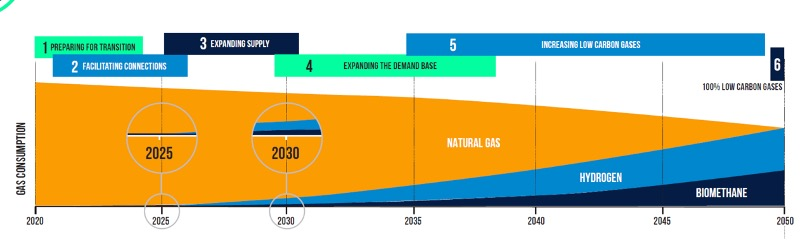
\includegraphics[scale=0.6]{futureforecaset.jpg}
			\caption{Pathway to Net Zero} 	% This needs a citation for the source I think
			\label{forecast}
		\end{figure}
		
		The end goal of the programme is that all gas end-users are supplied with hydrogen and/or biomethane, and natural gas is no longer used. Although it is difficult to predict whether this timeline will be met, the programme has set out clear deliverables through close consultation with the gas distributors and regulatory bodies. Therefore, it is reasonable to expect this timeline to be followed. 

		
		\textbf{Impact on us}\\
		Overall, the traditional gas pipeline industry is secure for at least the next 20 years in which time the use of natural gas will be far larger than that of green gases. After this period, the use of natural gas is expected to decelerate more rapidly. Despite this, a shift from natural gas to green gas is not necessarily bad for our business given that we will have developed the complex technology needed to navigate and map pipeline. \\
	    \hspace*{3ex}There appears to be three main challenges in the long term. Firstly, one challenge for our business could be the fact that transporting hydrogen requires the use of new pipeline materials and heavy pumps. Therefore, the inspection methods of our robot must be repurposed for use on materials such as fiber reinforced polymer. Another challenge is that due to the rapid installment of modern pipelines, the frequency of damage could be far lower than the currently used steel pipes. This in turn would reduce the amount of pipe inspection required. Although given the lower ignition temperature of Hydrogen compared to natural gas, there may be more enhanced regulation in the future. Finally, from \figref{forecast} it is expected that the total use of gas is expected to decrease gradually. This would place pressure on the gas suppliers, which would eventually be passed on to us. 
		
		\section{Competitor Analysis}
		
		\subsection[Project GRAID]{Project GRAID - Louis Emanuel}
			One significant competitor operating in the in-pipe inspection industry is Gas Robot Agile Inspection Device (GRAID). The robot is a joint project by the National Grid and three SMEs. As with our robot, it is targeting the live gas pipe market and aims to be able to navigate complex geometries. Therefore, it is necessary to perform the following SWOT analysis on the company. \\
			
			\textbf{Strengths} \\
			Project GRAID's key strength is its ongoing partnership with the National Grid. Although the National grid sold off its distribution network as Cadent, its history in the industry and extensive knowledge is an undeniable advantage for Synthotech. Further, Synthotech has previously received a voluntary contribution of £243,000 from the National Grid. This financial backing reduces the need for high interest loans which will be a significant fixed cost and barrier for new entrants. \\
		    \hspace*{3ex}Another significant strength of the GRAID project robot is its strong technical performance. Whilst CISBOT can operate at 99 psi, GRAID is capable of operating up to pressures of to 1450 psi. And although the distribution pipeline usually operates at pressures below 200 psi, this offers an advantage as it can inspect all pipes regardless of pressure levels. Further, as we progress to the use of hydrogen gas which will require higher distribution pressures due to its lower energy density, the need to inspect higher pressure pipes will make GRAID more competitive. 
	        
	        \textbf{Weaknesses}\\
	        Despite GRAID’s success, it does have weaknesses that could inhibit the success of the firm moving forward. Firstly, despite its partnership with the National Grid, GRAID is not partnered with an established gas network like CISBOT is with Cadent. This presents a challenge as ultimately, the robot must be sold or leased to these gas networks in order to generate revenue. \\
	        \hspace*{3ex}Another weakness lies in the fact that along with the National grid, Synthotech is also partnered with three other SMEs as part of the GRAID project. Although it could be argued that this brings more knowledge to the project, the heavily regulated gas distribution industry is slow enough, and so having multiple significant shareholders could slow down decision making significantly. This is significant given GRAID is already lagging behind first mover CISBOT. In fact, while CISBOT is already operational, GRAID is still undergoing testing. Therefore, any further delays in taking GRAID to market would significantly damage its long term prospects as CISBOT continues to consolidate its position in the market. \\
	        \textbf{Opportunities}\\
	        One area of opportunity is in the hydrogen gas pipeline refit that is currency being considered. As we transition to green gases, a full assessment of current gas distribution assets is required. This is particularly relevant for GRAID as given the National Grid has received significant funding from the Net Zero development funding to finance projects, the National Grid will have preference for using the inspection robot it partnered to manufacture. \\
	        \textbf{Threats} \\
	        One significant threat to GRAID is the rising customer loyalty in the pipe inspection market. For example, through CISBOT's partnership with Cadent, who is the largest gas distributor in the UK, it is unlikely Cadent will invest in another robot unless it provides distinct capabilities that CISBOT cannot offer. Another potential threat arises from the projected decrease in gas demand demonstrated in \figref{forecast}. If the market size decreases, the competition GRAID experiences will increase as the only way to boost revenue will be to gain market share.
	        
     \section[Business Risk Assessment]{Business Risk Assessment - Jim Laney}
     	
     	In order to assess how suitable the business was to take forward, several risks were considered for both severity and likelihood.
     	\\
     	Due to the large initial cost to create a robot, the company is particularly vulnerable to economic downturn.
     	As well as this, the first year or two will have high spending, and the business will most likely operate at a loss, which can be alleviated by ensuring a partnership with one of the gas networks.
     	Also, it is important to remain aware of the risk of similar products coming to market at the same time as the robot, since these will take away from the number of jobs which the robot can embark on.
     	Once again, partnering with a gas network will help to reduce the risk of this, allowing the company to be more confident in the projected revenue for the first few years.
     	Another factor which allows us to be more robustly able to deal with financial issues is the fact that the company produces a single product, which is much less likely to fail due to the significant investment in research and development, and a customer base where the industry is almost monopolistic.
     	\\
     	Another substantial business risk is the regulation and safety concerns around working within gas pipelines.
     	While the robot has been designed to meet all current UK regulations, there  is always a risk of the introduction of new legislation which may limit the robot effectiveness.
     	As well as this, gas networks are considered to be at fault if a third party causes damage, if it can be shown that they have not "exercised all due diligence"\supercite{books1996guide}, and as such it is imperative that the robot conforms to all regulations strictly.
     	As well as this, the high level of regulation of the gas industry makes moving into new markets a significantly more difficult process, as new regulations have to be followed, and new standards must be checked and followed.
     	This problem is further exacerbated by the fact that other markets, such as the United States, have regulations and standards which differ between states\supercite{pless2011making}.
     	\\
     	Another risk to the company is that of data security.
     	Since the robot stores data which could be used for nefarious purposes, it is important that any data collected is stored securely.
     	As well as this there is a chance that the data is lost when the robot is returning from the inspection run, especially if the robot gets stuck inside the pipes.
     	As well as this, employee and customer information must also be securely stored in order to conform with General Data Protection Regulations.
     	However, the possible effects of a data breach would be catastrophic, since there are such a small number of possible customers, meaning a reputation for safety and reliability is increasingly important.
     	\\
     	There are also a few operational risks when operating the robot which must be considered.
     	It is possible for the robot to get stuck in a pipe while inspecting, and extraction methods, such as using the communications wire or remotely controlling the robot, should be considered.
     	As well as this, the business model assumes there are only a small number of robots built, and thus there is also a risk that all robots in stock become damaged or otherwise inoperable.
     	However, the expected low number of jobs which are expected to be undertaken means that this is an unlikely outcome, as there should always be sufficient time for at least one robot to be operational.
     	\\
     	There is also the ongoing risk that, assuming that the robot becomes the standard industry solutions for inspection, the company becomes complacent.
     	As such, it is important to explore the future of the robot while operating the inspection service, and evaluate the likelihood of a reduction in the use of fossil fuels, and future moves to other sustainable technologies.
     	For example, in the case of a move to hydrogen pipes, the transition is fairly simple as similar, or possibly even the same, gas networks will be used to transport the hydrogen around.
     	If the potential of further development of the robot is considered a viable option, it is important to monitor the rate of development to make sure that development is still in the steep section of the technological S-curve\supercite{christensen1998innovation}, and be prepared to switch to a new development curve or diversify the company's portfolio with an additional product.
     	
	
	\pagebreak		% Temp page break for references - might end up replacing with a multicolumn environment later
	
	% In order to make a reference to an entry in the bibliography, use \cite{}
	% TexStudio will suggest names from the bib file - not sure about overleaf but otherwise use the first entry in the string
	% Make sure bibliography is set to use BibTex rather than BibLatex
	% Currently using google scholar default ids - should help prevent duplication of references but will need to be checked
	
	% For websites use the misc tag - see how I've done rsproLinear - the author is in 2 brackets so it doesn't get made into initials
	
	%\nocite{*} 				% By default Latex will not show uncited references, uncomment this line to show all references in the bib file
	
	\begingroup\onehalfspacing
		{\small
			\bibliographystyle{ieeetr}
			\bibliography{3YPbib}
		}
	\endgroup

\end{document}